% !TeX encoding = UTF-8
%DIF LATEXDIFF DIFFERENCE FILE
%DIF DEL /home/uav/00gao_xueshu/DT_PAPER/XIU_tase_paper_V1/main_before_reviewer_revision_20260718.tex   Sat Jul 18 15:44:35 2026
%DIF ADD revision_autoresearch/paper_v10_integration/work/main_revised.tex                              Wed Jul 22 15:30:15 2026
% !TeX program = pdflatex
% IEEEtran Journal Template -- Migrated from Elsevier cja-template.tex
\documentclass[lettersize,journal]{IEEEtran}

%% ---- Packages (only those compatible with IEEEtran) ----
\usepackage{amsmath,amsfonts,amssymb}
\usepackage{algorithm}
\usepackage{algorithmic}    % IEEEtran recommends algorithmic (not algorithmicx)
\usepackage{array}
\usepackage{bm}
\usepackage{booktabs}
\usepackage{multirow}
\usepackage{graphicx}
\usepackage{url}
\usepackage{cite}           % IEEE-style numeric citations
\usepackage{textcomp}
\usepackage{stfloats}       % allows figure* at bottom
%DIF 19a19
\usepackage{placeins}       % keeps each method--case result group together %DIF > 
%DIF -------
% \usepackage[caption=false,font=normalsize,labelfont=sf,textfont=sf]{subfig}
\usepackage[caption=false,font=footnotesize,labelfont=sf,textfont=sf]{subfig}
\usepackage{siunitx}

% theorem/lemma environments
\newtheorem{theorem}{Theorem}
\newtheorem{lemma}{Lemma}

\hyphenation{op-tical net-works semi-conduc-tor IEEE-Xplore}

% ----------------------------------------------------------------
%DIF PREAMBLE EXTENSION ADDED BY LATEXDIFF
%DIF CFONT PREAMBLE %DIF PREAMBLE
\RequirePackage{color}\definecolor{RED}{rgb}{1,0,0}\definecolor{BLUE}{rgb}{0,0,1} %DIF PREAMBLE
\DeclareOldFontCommand{\sf}{\normalfont\sffamily}{\mathsf} %DIF PREAMBLE
\providecommand{\DIFadd}[1]{{\protect\color{blue} #1}} %DIF PREAMBLE
\providecommand{\DIFdel}[1]{} %DIF PREAMBLE
%DIF SAFE PREAMBLE %DIF PREAMBLE
\providecommand{\DIFaddbegin}{} %DIF PREAMBLE
\providecommand{\DIFaddend}{} %DIF PREAMBLE
\providecommand{\DIFdelbegin}{} %DIF PREAMBLE
\providecommand{\DIFdelend}{} %DIF PREAMBLE
\providecommand{\DIFmodbegin}{} %DIF PREAMBLE
\providecommand{\DIFmodend}{} %DIF PREAMBLE
%DIF FLOATSAFE PREAMBLE %DIF PREAMBLE
\providecommand{\DIFaddFL}[1]{\DIFadd{#1}} %DIF PREAMBLE
\providecommand{\DIFdelFL}[1]{\DIFdel{#1}} %DIF PREAMBLE
\providecommand{\DIFaddbeginFL}{} %DIF PREAMBLE
\providecommand{\DIFaddendFL}{} %DIF PREAMBLE
\providecommand{\DIFdelbeginFL}{} %DIF PREAMBLE
\providecommand{\DIFdelendFL}{} %DIF PREAMBLE
%DIF LISTINGS PREAMBLE %DIF PREAMBLE
\RequirePackage{listings} %DIF PREAMBLE
\RequirePackage{color} %DIF PREAMBLE
\lstdefinelanguage{DIFcode}{ %DIF PREAMBLE
%DIF DIFCODE_CFONT %DIF PREAMBLE
  moredelim=[il][\color{red}\scriptsize]{\%DIF\ <\ }, %DIF PREAMBLE
  moredelim=[il][\color{blue}\sffamily]{\%DIF\ >\ } %DIF PREAMBLE
} %DIF PREAMBLE
\lstdefinestyle{DIFverbatimstyle}{ %DIF PREAMBLE
	language=DIFcode, %DIF PREAMBLE
	basicstyle=\ttfamily, %DIF PREAMBLE
	columns=fullflexible, %DIF PREAMBLE
	keepspaces=true %DIF PREAMBLE
} %DIF PREAMBLE
\lstnewenvironment{DIFverbatim}{\lstset{style=DIFverbatimstyle}}{} %DIF PREAMBLE
\lstnewenvironment{DIFverbatim*}{\lstset{style=DIFverbatimstyle,showspaces=true}}{} %DIF PREAMBLE
%DIF END PREAMBLE EXTENSION ADDED BY LATEXDIFF

\begin{document}

% ---- Title ----
% \title{Multi-Agent Reinforcement Learning-Based Cooperative Interception Strategy
%   for Maneuvering Swarm Attack Targets with Considering Target Assignment}

% \title{Trust-Aware Multi-Agent Reinforcement Learning-Based Cooperative Interception Strategy for Maneuvering Swarm Attack Targets Considering Rapid Consensus Target Assignment}
\title{Trust-Aware Multi-Agent Reinforcement Learning-Based Cooperative Interception Strategy for Maneuvering Swarms with Target Assignment}

% ---- Authors ----
% \author{Shuyi~Gao,~Defu~Lin,~Duo~Zheng,~and~Zhichen~Chu%
% \thanks{S. Gao, D. Lin, D. Zheng, and Z. Chu are with the School of Aerospace
% Engineering, Beijing Institute of Technology, Beijing 100081, China
% (e-mail: zhengduohello@126.com).}%
% \thanks{Manuscript received 2025.}}

%----双盲投稿--
\author{}
\markboth{Under review}%
{Anonymous Submission}

% ---- Running heads ----
\markboth{IEEE Transactions on Automation Science and Engineering}%
{Gao \MakeLowercase{\textit{et al.}}: MARL-Based Cooperative Interception for Maneuvering Swarm Targets}

\maketitle

% ---- Abstract ----
\begin{abstract}
The swarm attack of unmanned aerial vehicles (UAVs) poses a significant threat to future
battlefield operations.
Achieving efficient and precise cooperative interception against attacking UAV swarms with
highly dynamic maneuvering capabilities and adaptive penetration strategies poses a critical
challenge for UAV interceptor swarms.
This study addresses the cooperative interception of maneuvering targets in swarm attacks by
decomposing the problem into two key tasks: target assignment and cooperative interception
guidance.
For target assignment, \DIFdelbegin \DIFdel{an }\DIFdelend \DIFaddbegin \DIFadd{a distributed consensus-based }\DIFaddend Improved Dung Beetle
Optimization (IDBO) algorithm is proposed to dynamically balance exploration
and exploitation \DIFdelbegin \DIFdel{, achieving highly efficient and rapid
assignments}\DIFdelend \DIFaddbegin \DIFadd{while reconciling capacity-constrained target bids among
neighboring interceptors}\DIFaddend .
% For cooperative interception guidance, a multi-agent deep reinforcement learning-based method
% is developed to achieve precise and time-coordinated interception of adversarial UAV swarms
% employing advanced penetration strategies.
% For cooperative interception guidance, a multi-agent deep reinforcement learning framework—augmented by kinematics-aware attention mechanisms and trust-modulated exploration—is developed to achieve precise and time-coordinated interception of adversarial UAV swarms employing advanced penetration strategies.
For cooperative interception guidance, an Attention-Residual and Trust-aware Multi-Agent Proximal Policy Optimization (ART-MAPPO) framework is developed to achieve precise and time-coordinated interception of adversarial UAV swarms employing advanced penetration strategies.
The simulation \DIFaddbegin \DIFadd{and hardware-in-the-loop (HIL) }\DIFaddend results validate the effectiveness
of the proposed intelligent cooperative interception method, demonstrating
superior convergence speed, robustness, and significantly improved interception
success rates in swarm UAV cooperative interception scenarios.
\end{abstract}

{\linespread{0.9}\selectfont
\hspace*{0.0em}\textbf{\textit{Note to Practitioners—}}\textbf{This paper is motivated by practical UAV swarm defense scenarios, where multiple interceptors must cooperatively engage maneuvering aerial targets under limited communication and onboard maneuver constraints. In such applications, target assignment and guidance are closely coupled, and conventional centralized approaches may be difficult to implement efficiently as the engagement scale increases. To address this issue, this paper develops a two-stage cooperative interception framework that combines distributed target assignment with a trust-aware multi-agent reinforcement learning guidance method. The proposed approach is intended to improve coordination consistency among interceptors assigned to the same target and to enhance robustness against target maneuvers while considering maneuver saturation and command smoothness. \DIFaddbegin \DIFadd{Three-dimensional simulation and a hardware-connected HIL campaign are used to evaluate the complete assignment-to-guidance chain under delay, noise, and packet loss. }\DIFaddend This work may be useful for practical large-scale multi-UAV interception and other cooperative autonomous systems requiring scalable distributed decision-making and coordinated guidance.}\par\vspace{0.5\baselineskip}
}

% ---- Keywords ----
\begin{IEEEkeywords}
Cooperative interception, deep reinforcement learning, centralized training with decentralized
execution, target assignment, UAV swarm.
\end{IEEEkeywords}

\begin{center}
\footnotesize\textcolor{blue}{Blue text indicates additions or replacements relative to the original manuscript.}
\end{center}


%% ===========================================================
\section{Introduction}
\label{sec:introduction}
\IEEEPARstart{A}{s} warfare evolves toward intelligent swarm operations, the likelihood of
encountering attacks from adversarial UAV swarms significantly increases during combat.
Consequently, the efficient interception of incoming swarm targets becomes a critical
imperative for future battlefield operations.
To address the challenge of cooperative interception against maneuvering attacking swarms with
adaptive penetration strategies, there is an urgent need to advance academic research in swarm
target interception technologies.
This study aims to enhance interceptors with intelligent cooperative interception capabilities,
enabling effective navigation of complex challenges in modern battlefield environments.

Multi-target cooperative interception encompasses two key tasks: target assignment and
cooperative interception.
The effectiveness of multi-target interception hinges on the optimality of target assignment,
establishing it as a primary focus in swarm target interception strategies.
As the number of UAVs increases, the complexity of target assignment escalates significantly,
resulting in a multi-constrained, multi-parameter optimization problem.
The objective is to develop a rapid and efficient target assignment method for allocating
specific attacking targets to interceptors in operational scenarios~\cite{KLINE2019226}.
The target assignment problem involves complex constraints, and the non-dominated sorting
algorithm can dynamically generate a set of reference points with good convergence and
distribution performance~\cite{WANG2025952,bai2024hybrid,zou2024moea}.
Moreover, employing an online operator selection mechanism can enhance the efficiency of the
algorithm~\cite{ahmad2024fuzzy,ming2024constrained}.
The target assignment problem can be solved using multi-information particle swarm optimization
to find the solution that yields the highest gain~\cite{mishra2015weapon,wei2020particle}.
Introducing information from surrounding particles can enhance the stability of the traditional
particle swarm algorithm while also addressing the issue of local convergence in the target
assignment problem~\cite{long2024improved}.
The genetic algorithm is a common approach for solving the target assignment
problem~\cite{he4914655modelling,li2020multi,sun2022multi,chang2018solving}, and a GA with a
novel crossover operator can further enhance algorithmic efficiency~\cite{weng2024diversity}.
Ant colony optimization is also an effective strategy for solving the target assignment
problem~\cite{li2024comprehensive}, and its combination with a greedy algorithm can improve
the accuracy of parallel computation~\cite{yi2024solving}.
Under multiple constraints, researchers have proposed various heuristic algorithms to solve the
target assignment problem, such as neural networks~\cite{li2024comprehensive}, auction
algorithm~\cite{wang2024collaborative}, tabu search~\cite{yao2024tabu}, simulated annealing
algorithm~\cite{khurshid2024hybrid}, VLSN~\cite{yue2024graph}.
However, in cooperative interception scenarios, the aforementioned algorithms struggle to
handle the highly dynamic nature of the battlefield due to their high time complexity, and they
fail to meet the dual requirements of both speed and optimality.

The effectiveness of the terminal guidance phase in multi-target interception is significantly
influenced by the cooperative guidance law, a critical factor requiring thorough consideration.
The target assignment strategy transforms swarm operations into a coordinated multi-to-one
interception problem, with current research focusing on three key areas: angular coordination,
temporal coordination, and intelligent cooperation.
Significant progress has been made in temporal coordination.
Classical proportional navigation-based guidance laws enable synchronized multi-missile attacks
on a single target~\cite{tao2024analytical}.
Adaptive control methods adjust attack timing based on real-time operational conditions, making
them suitable for intercepting maneuvering targets~\cite{wang2025generalized,zhang2022multiple}.
Sliding Mode Control (SMC) is widely adopted for cooperative
interception~\cite{sinha2020supertwisting}, with SMC incorporating miss distance and attack
time constraints enhancing interception
accuracy~\cite{shen2025three,jin2025cooperative,hu2019sliding}.
Considerable research has also been conducted on angular coordination.
From a traditional control perspective, backstepping control~\cite{li2024adaptive} and
leader-follower cooperative methods~\cite{he2017impact} significantly improve interception
efficiency.
SMC with angular constraints is prevalent in cooperative interception, encompassing approaches
based on impact angle constraints~\cite{wang2025hybrid} and line-of-sight angle
constraints~\cite{li2024near}.
Optimal control methods applied to impact angle-constrained cooperative guidance enhance
precision by integrating impact angle and line-of-sight angle
constraints~\cite{wang2025adaptive,tao2023optimal}.

Recent advancements in intelligent technologies have driven extensive research into cooperative
interception strategies for UAV swarms, with intelligent algorithms demonstrating substantial
potential in addressing complex multi-target scenarios~\cite{chen2024enhanced,wu2020collaborative}.
Optimization-based approaches, such as Particle Swarm Optimization (PSO), excel in
collaborative attack problems by autonomously optimizing resource allocation and maximizing
operational efficiency~\cite{zhao2024hierarchical,wu2020collaborative}.
Search-based algorithms, like A*~\cite{liao2024research}, enable efficient path planning for
coordinated attacks.
Control-based methods, including Model Predictive Control
(MPC)~\cite{kim2024adaptive}, provide robust guidance under dynamic constraints.
Moreover, the integration of neural networks with reinforcement learning, particularly deep
reinforcement learning (DRL), enhances the adaptability and intelligence of interception
strategies~\cite{luo2022uav,zhan2022multiple,wang2021uav}.
DRL enables UAV swarms to learn complex policies from high-dimensional data, optimizing target
assignment and maneuvering in real-time to counter maneuvering targets~\cite{sun2024memory}.
In contrast, conventional cooperative interception guidance methods rely heavily on
linearization and simplifying assumptions to design feasible guidance laws~\cite{zhao2025global}.
These methods often struggle to address the complexity of dynamic, non-linear environments
involving maneuvering swarm targets.
Data-driven intelligent cooperative interception methods, by contrast, leverage extensive
datasets to learn adaptive strategies, significantly reducing dependence on restrictive
assumptions~\cite{fainkich2025cooperative}.
By modeling complex interactions through neural networks and DRL, these methods achieve greater
robustness and flexibility.
Despite advancements, intelligent cooperative interception methods struggle with maneuvering
swarm targets in complex dynamic environments due to limited model generalization, low training
efficiency, and low interception success rates, particularly in large-scale swarm combat
requiring precise temporal coordination~\cite{horyna2023decentralized}.
Addressing these challenges requires further research into scalable, generalizable, and
efficient algorithms to fully realize the potential of intelligent cooperative interception.

In summary, existing cooperative interception methods for countering attacking UAV swarms with
adaptive penetration capabilities suffer from low interception success rates in complex dynamic
environments.
Specifically, target assignment methods exhibit low allocation efficiency, while cooperative
interception guidance strategies struggle with terminal overload saturation and insufficient
adaptability to dynamic target maneuvers in practical scenarios, hindering effective swarm
coordination.
Consequently, more research is necessary to address these challenges.

This study proposes a swarm cooperative interception method based on multi-agent reinforcement
learning and IDBO algorithm, enhancing target assignment efficiency and guidance strategy
performance to achieve precise and efficient interception of maneuvering targets.
The proposed intelligent cooperative interception algorithm offers the following advantages.

\begin{enumerate}
\item A distributed consensus-based target assignment scheme is proposed, which integrates an
improved Dung Beetle Optimization (IDBO) algorithm with a combat-dominance assessment model.
This design supports rapid many-to-one allocation under limited communication, leading to more
efficient and reliable target assignment for cooperative interception.

\item ART-MAPPO is proposed as a CTDE-based cooperative interception guidance learning
framework, which employs an attention--residual feature extractor and a GRU temporal encoder,
and uses trust-modulated exploration together with dual-clip PPO and adaptive KL
regularization for stable policy learning. This design improves convergence behavior and
training efficiency in highly maneuverable swarm-adversarial environments.

\item A task-oriented reward design and training stabilization strategy are incorporated into
the cooperative interception framework to support time-coordinated guidance under bounded
overload commands. Rather than treating reward shaping or dual-clip PPO as standalone
methodological novelties, this work uses them as task-adapted components that couple target
approach, terminal interception, temporal coordination, and control-effort regularization in a
large-scale maneuvering swarm scenario. \DIFaddbegin \DIFadd{The complete two-stage method is
evaluated in three-dimensional simulation and in a hardware-connected HIL
configuration.
}\DIFaddend \end{enumerate}

The paper is structured as follows: Section~\ref{sec:method} presents relevant problem modeling and foundational theory. Section~\ref{sec:target_assignment} and Section~\ref{sec:cooperative_algorithm} provide a detailed description of our approach, including its framework, modules, algorithms, and rationale. Section~\ref{sec:simulation} covers experiments, results, and discussions. Lastly, Section~\ref{sec:conclusion} summarizes the paper and outlines future directions.

%% ===========================================================
\section{Backgrounds and Preliminaries}
\label{sec:method}

In this section, we first introduce the modeling of multi-target interception of UAVs, and
then review reinforcement learning methods.

\subsection{Problem Modeling}

The multi-target intelligent interception problem can be decomposed into two subproblems:
target assignment and intelligent cooperative interception, with the swarm combat scenario
illustrated in Fig.~\ref{fenpei}.
In this scenario, the attacking swarm aims to penetrate a high-value target area, while the
defending swarm seeks to fully intercept the incoming UAVs.
During the target assignment phase, the defending swarm assesses its own flight status and
that of the attacking swarm using onboard sensors, subsequently allocating each defender to an
appropriate interception target via the target assignment strategy.
In the intelligent cooperative interception phase, defenders assigned to the same target employ
coordinated maneuvering strategies to intercept and neutralize the target.

\begin{figure}[!t]
\centering
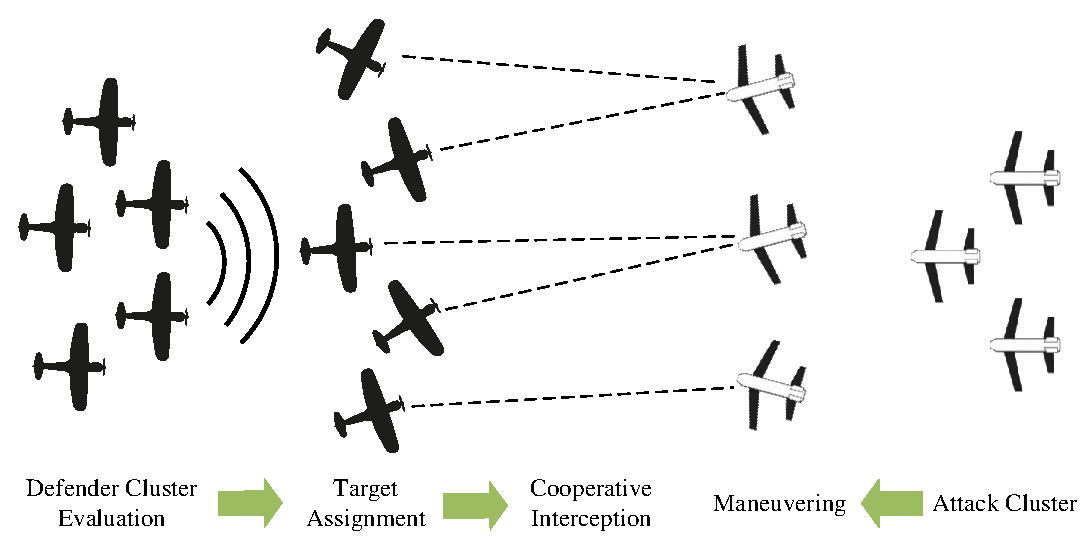
\includegraphics[width=2.8in]{fenpei.pdf}
\caption{Cluster target interception problem.}
\label{fenpei}
\end{figure}

The object of study in this paper is the fixed-wing UAV\DIFdelbegin \DIFdel{, and the interception problem is
reduced to a two-dimensional horizontal plane as shown in }\DIFdelend \DIFaddbegin \DIFadd{. }\DIFaddend Fig.~\ref{jianmo}
\DIFdelbegin \DIFdel{without loss of
generality}\DIFdelend \DIFaddbegin \DIFadd{shows the horizontal projection used to define the heading and line-of-sight
angles, whereas the simulation and HIL evaluations propagate the complete
three-dimensional position and velocity}\DIFaddend .

\begin{figure}[!t]
\centering
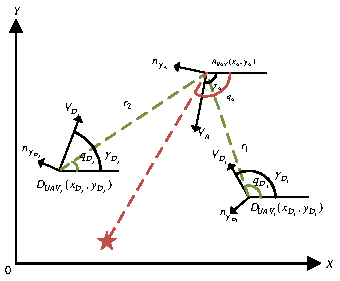
\includegraphics[width=2.6in]{pic02.pdf}
\caption{Schematic diagram of confrontation and interception.}
\label{jianmo}
\end{figure}

The \DIFaddbegin \DIFadd{three-dimensional point-mass }\DIFaddend kinematic model of a single UAV \DIFdelbegin \DIFdel{can be simplified as
}%DIFDELCMD < \begin{equation}
%DIFDELCMD < \label{yundongxue}
%DIFDELCMD < \left\{\begin{matrix}\dot{x} =V\cos\gamma \\
%DIFDELCMD < \dot{y} =V\sin\gamma \end{matrix}\right.
%DIFDELCMD < \end{equation}%%%
\DIFdelend \DIFaddbegin \DIFadd{is
}\begin{equation}
\label{yundongxue}
\left\{\begin{matrix}
\dot{x}=V\cos\vartheta\cos\gamma,\\
\dot{y}=V\cos\vartheta\sin\gamma,\\
\dot{z}=V\sin\vartheta
\end{matrix}\right.
\end{equation}\DIFaddend 
where \DIFdelbegin \DIFdel{\emph{x}}\DIFdelend \DIFaddbegin \DIFadd{\((x,y,z)\) are the three-dimensional position coordinates}\DIFaddend , \DIFdelbegin \DIFdel{\emph{y} is the position coordinates of the UAV in two-dimensional space, \emph{V} }\DIFdelend \DIFaddbegin \DIFadd{\(V\) }\DIFaddend is
the velocity magnitude\DIFdelbegin \DIFdel{of the UAV, and $\gamma$ is
the navigation }\DIFdelend \DIFaddbegin \DIFadd{, \(\gamma\) is the heading angle, and \(\vartheta\) is
the flight-path }\DIFaddend angle.

In an interception mission, the relative motion relationship between the attacking and
defending UAVs can be described as:
\DIFdelbegin %DIFDELCMD < \begin{equation}
%DIFDELCMD < \label{gongfang}
%DIFDELCMD < \left\{\begin{matrix}\dot{r} =V_{A}\cos(\gamma_{A}-q)-V_{D}\cos(\gamma_{D}-q) \\
%DIFDELCMD < r\dot{q} =V_{A}\sin(\gamma_{A}-q)-V_{D}\sin(\gamma_{D}-q)\end{matrix}\right.
%DIFDELCMD < \end{equation}%%%
\DIFdelend \DIFaddbegin \begin{equation}
\label{gongfang}
\begin{split}
\mathbf r_{AD}&=\mathbf p_A-\mathbf p_D,\qquad
r=\|\mathbf r_{AD}\|_2,\qquad
\boldsymbol{\ell}_{AD}=\mathbf r_{AD}/r,\\
\dot r&=\boldsymbol{\ell}_{AD}^{\top}(\mathbf v_A-\mathbf v_D).
\end{split}
\end{equation}\DIFaddend 
\DIFdelbegin \DIFdel{where $r$ is the }\DIFdelend \DIFaddbegin \DIFadd{Here \(r\) is the three-dimensional }\DIFaddend inter-UAV distance \DIFdelbegin \DIFdel{, $q$ is the line-of-sight angle
, $V_{A}$ ($V_{D}$) is the velocity of the attacking (defending) UAV, and $\gamma_{A}$ ($\gamma_{D}$) is the
corresponding heading angle}\DIFdelend \DIFaddbegin \DIFadd{and
\(\boldsymbol{\ell}_{AD}\) is the LOS unit vector. The horizontal LOS angle
\(q\) used below is the azimuth of this vector}\DIFaddend .

In the interception phase, the relationship between UAV flight state and acceleration is:
\DIFdelbegin %DIFDELCMD < \begin{equation}
%DIFDELCMD < \label{guozai}
%DIFDELCMD < \left\{\begin{matrix}\dot{V} =n_{x} g \\
%DIFDELCMD < \dot{\gamma} =n_{y}g/V \end{matrix}\right.
%DIFDELCMD < \end{equation}%%%
\DIFdelend \DIFaddbegin \begin{equation}
\label{guozai}
\left\{\begin{matrix}
\dot{V}=n_xg,\\
\dot{\gamma}=n_yg/(V\cos\vartheta),\\
\dot{\vartheta}=n_zg/V
\end{matrix}\right.
\end{equation}\DIFaddend 
where \DIFdelbegin \DIFdel{$n_{x}$ }\DIFdelend \DIFaddbegin \DIFadd{\(n_x\) }\DIFaddend is the axial \DIFdelbegin \DIFdel{acceleration command, $n_{y}$ is the
normal acceleration command, and $g$ is the }\DIFdelend \DIFaddbegin \DIFadd{load command, \(n_y\) and \(n_z\) are the
horizontal and vertical normal load commands, and \(g\) is }\DIFaddend gravitational
acceleration.
In the multi-agent setting of Section~\ref{sec:cooperative_algorithm}, these variables carry
an agent subscript $i$.

During cooperative interception, the remaining impact time is defined as:
\begin{equation}
\label{shijian}
t_{go}=\frac{r}{\left|\dot{r}\right|}
\end{equation}

The Zero-Effort Miss (ZEM) is defined as:
\DIFdelbegin %DIFDELCMD < \begin{equation}
%DIFDELCMD < \label{ZEM}
%DIFDELCMD < ZEM = \frac{r^{2}\cdot\dot{q}}{\left|\dot{r}\right|}
%DIFDELCMD < \end{equation}%%%
\DIFdelend \DIFaddbegin \begin{equation}
\label{ZEM}
\operatorname{ZEM}
=\left\|\mathbf r_{AD}
+(\mathbf v_A-\mathbf v_D)t_{go}\right\|_2
\end{equation}\DIFaddend 

\subsection{Reinforcement Learning}

Reinforcement learning (RL) is built on the Markov Decision Process (MDP), comprising state
space $\mathcal{S}$, action space $\mathcal{A}$, reward function $R$, policy $\pi$, and state
transition function $P$.
At each step, the agent selects action $a$ from state $s$, receives reward $r$, and
transitions to $s'$.
The key value functions are:
\begin{equation}
\label{RLV}
V^{\pi}(s)=E_{\pi}\left[\sum_{t=0}^{\infty}\gamma_{\mathrm{RL}}^{t}r_{t}\mid s_{0}=s\right]
\end{equation}
\begin{equation}
\label{RLQ}
Q^{\pi}(s,a)=E_{\pi}\left[\sum_{t=0}^{\infty}\gamma_{\mathrm{RL}}^{t}r_{t}\mid s_{0}=s,a_{0}=a\right]
\end{equation}
where $\gamma_{\mathrm{RL}}\in[0,1]$ is the discount factor.






\section{Target Assignment via Distributed Consensus-Based IDBO Algorithm}
\label{sec:target_assignment}

This section formulates the cooperative target assignment as a weighted bipartite matching problem and solves it via an Improved Dung Beetle Optimization (IDBO) algorithm embedded in a distributed consensus framework.

\subsection{Problem Formulation}
\label{subsec:problem_formulation}

Let $\mathcal{U} = \{u_1, u_2, \dots, u_M\}$ and $\mathcal{T} = \{t_1, t_2, \dots, t_N\}$ denote the interceptor and target sets, respectively. Figure \ref{km} illustrates the bipartite assignment structure.

\begin{figure}[!t]
\centering
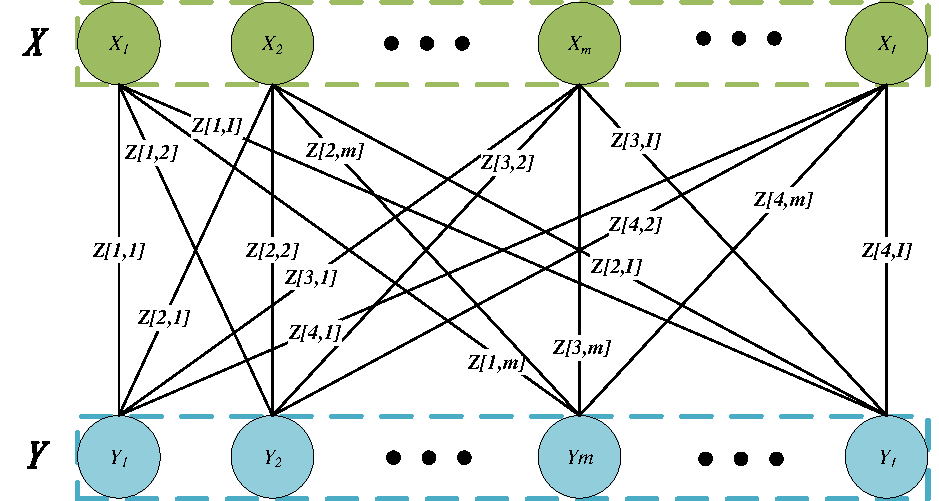
\includegraphics[width=2.5in]{KM1.pdf}
\caption{Schematic diagram of weighted dichotomy.}
\label{km}
\end{figure}

The binary decision variable $X_{ij}=1$ if UAV $u_i$ is assigned to target $t_j$ and 0 otherwise. The edge weight $P_{ij}$ quantifies the interception probability. Intuitively, a desirable interceptor-target edge should have both a small predicted miss tendency and a favorable heading geometry; therefore, the weight combines ZEM-based feasibility and angular advantage:

\begin{equation}
\label{eq:interception_probability}
P_{ij} = w_1 \cdot P_{\text{ZEM}}(i,j) + w_2 \cdot P_{\sigma}(i,j)
\end{equation}
where $w_1 + w_2 = 1$, $w_1, w_2 \geq 0$. The Zero-Effort Miss (ZEM) component is:

\begin{equation}
\label{eq:zem_prob}
P_{\text{ZEM}}(i,j) = \exp\left[-\frac{1}{2}\left(\frac{\text{ZEM}(i,j)}{\overline{\text{ZEM}}}\right)^2\right]
\end{equation}
where $\overline{\text{ZEM}} = \frac{1}{MN}\sum_{i=1}^{M}\sum_{j=1}^{N} \text{ZEM}(i,j)$.

The angular advantage component is:

\begin{equation}
\label{eq:angular_prob}
P_{\sigma}(i,j) = \exp\left[-\frac{1}{2}\left(\frac{S_{\sigma}(i,j)}{\overline{S_{\sigma}}}\right)^2\right]
\end{equation}
where $\overline{S_{\sigma}} = \frac{1}{MN}\sum_{i=1}^{M}\sum_{j=1}^{N} S_{\sigma}(i,j)$, with $S_{\sigma}(i,j) = |\gamma_{ij} - q_{ij}|$ denoting the heading error. The assignment objective below converts the tactical goal of ``neutralize as many attackers as possible'' into a survival-probability minimization problem. Under many-to-one assignment, each additional capable interceptor assigned to the same target multiplies that target's survival probability by another failure term:

\begin{equation}
\label{eq:optimization_formulation}
\begin{aligned}
\min_{\mathbf{X}} \quad & J = \sum_{j=1}^{N} \left[ \prod_{i=1}^{M} \left(1 - P_{ij}\right)^{X_{ij}} \right] \\
\text{s.t.} \quad & \sum_{j=1}^{N} X_{ij} = 1, \quad \forall i \in \{1,\dots,M\} \\
& \sum_{i=1}^{M} X_{ij} \geq 1, \quad \forall j \in \{1,\dots,N\} \\
& \sum_{i=1}^{M} X_{ij} \leq L_{\max}, \quad \forall j \in \{1,\dots,N\} \\
& X_{ij} \in \{0,1\}, \quad \forall i,j
\end{aligned}
\end{equation}
where $\prod_{i=1}^{M} (1 - P_{ij})^{X_{ij}}$ yields the survival probability of $t_j$, which decreases geometrically with the number of assigned interceptors.

\subsection{Distributed Consensus-Based IDBO Framework}
\label{subsec:idbo_algorithm}

The IDBO algorithm solves \eqref{eq:optimization_formulation} by alternating between local metaheuristic optimization and distributed consensus-based conflict resolution. Instead of requiring a single centralized optimizer to decide all binary assignments, each UAV first searches for promising targets locally and then reconciles conflicts with its neighbors. Let $\mathbf{X}^{(k)} = [x_{ij}^{(k)}] \in \{0,1\}^{M \times N}$ denote the assignment matrix at iteration $k$, where $x_{ij}^{(k)}=1$ indicates UAV $u_i$ is assigned to target $t_j$. The integrated optimization is:

\begin{equation}
\label{eq:hierarchical}
\mathcal{A}_{\text{IDBO}}^{(k+1)} = \mathcal{G}_{\text{consensus}} \circ \mathcal{F}_{\text{optimizer}} \left( \mathbf{X}^{(k)}, \boldsymbol{\Theta}^{(k)} \right)
\end{equation}
where $\mathcal{F}_{\text{optimizer}}$ denotes the improved DBO operator and $\mathcal{G}_{\text{consensus}}$ the consensus-based conflict resolver. The parameter set $\boldsymbol{\Theta}^{(k)} = \{\mathbf{A}^{(k)}, \mathbf{P}^{(k)}, \mathbf{V}^{(k)}\}$ aggregates the adversarial advantage, interception probability, and velocity matrices at iteration $k$.

Each UAV $u_i$ maintains a preference vector $\mathbf{x}_i \in [0,1]^{N}$, where $x_{ij}$ encodes the normalized affinity for target $t_j$. The fitness function acts as a local utility: it rewards targets that are likely and tactically favorable to intercept, while discouraging choices that would overload the same target with too many defenders. It is defined as:

\begin{equation}
\label{eq:idbo_fitness}
\begin{split}
\mathcal{F}_i(\mathbf{x}_i) =& \sum_{j=1}^{N} \sigma(x_{ij}) \cdot P_{ij} + \lambda_1 \sum_{j=1}^{N} \sigma(x_{ij}) \cdot A_{ij} \\
&- \lambda_2 \sum_{j=1}^{N} \Psi_{ij}(\mathbf{x}_i, \hat{\mathbf{X}}_{\mathcal{N}_i})
\end{split}
\end{equation}
where the three terms correspond to interception probability, adversarial advantage ($\lambda_1$-weighted), and an over-saturation penalty ($\lambda_2$-weighted). The penalty $\Psi_{ij}$ is:

\begin{equation}
\label{eq:saturation_penalty}
\begin{split}
\Psi_{ij}(\mathbf{x}_i, \hat{\mathbf{X}}_{\mathcal{N}_i}) =& \sigma(x_{ij}) \cdot \max\Biggl(0, \Biggl(\sum_{k \in \mathcal{N}_i, k \neq i} \sigma(\hat{x}_{kj}) \\
&+ \sigma(x_{ij})\Biggr) - L_{\max}\Biggr)
\end{split}
\end{equation}
where $\mathcal{N}_i$ is the neighbor set of $u_i$, $\hat{x}_{kj}$ the estimated preference of neighbor $u_k$, and $L_{\max}$ the per-target interceptor capacity. The penalty activates only when the estimated assignment count exceeds $L_{\max}$, steering the swarm toward capacity-feasible solutions.

The adversarial advantage $A_{ij}$ provides the tactical bias used by the optimizer. A large value indicates that interceptor $u_i$ can reach target $t_j$ quickly, with compatible velocity and favorable geometry, while facing limited competition from other interceptors:

\begin{equation}
\label{eq:adversarial_advantage}
\begin{split}
A_{ij} =& \exp\left(-\frac{\Delta t_{ij}}{T_{\max}}\right) \cdot \left(1 - \frac{\|\mathbf{v}_i - \mathbf{v}_j\|_2}{v_{\max}}\right) \\
&\cdot \max\left(0, \cos(\theta_{ij})\right) - \sum_{k\neq i} \frac{P_{kj}}{P_{ij} + P_{kj}} \cdot \sigma(\hat{x}_{kj})
\end{split}
\end{equation}
where $\Delta t_{ij}$ is the estimated time-to-intercept; $\mathbf{p}_i=[x_i, y_i]^\top$ and $\mathbf{v}_i=[\dot{x}_i, \dot{y}_i]^\top$ denote the position and velocity vectors of interceptor $u_i$; $\mathbf{p}_j=[x_j, y_j]^\top$ and $\mathbf{v}_j=[\dot{x}_j, \dot{y}_j]^\top$ denote the position and velocity vectors of target $t_j$; $\theta_{ij}$ is the aspect angle associated with the engagement geometry between $u_i$ and $t_j$; and $v_{\max}$ is the maximum reference speed used for normalization. The three multiplicative factors encode temporal, energetic, and geometric advantage, respectively, while the subtracted term penalizes competition from other interceptors with high preferences for the same target.

The IDBO update mechanism enhances the standard DBO through four adversarial-information-driven operations. In intuitive terms, rolling exploits the local fitness gradient, dancing injects controlled perturbations, breeding pulls candidates toward elite preferences, and stealing transfers useful target preferences among competing UAVs:

\begin{align}
\text{Rolling:} \quad & \mathbf{x}_i^{(t+1)} = \mathbf{x}_i^{(t)} + \alpha \cdot \nabla_{\mathbf{x}_i} \mathcal{F}_i(\mathbf{x}_i^{(t)}) \circ \mathbf{A}_i \nonumber \\
& \quad + \beta \cdot \mathbf{r}_i \cdot \exp\left(-\frac{t}{T}\right) \label{eq:rolling_update} \\
\text{Dancing:} \quad & \mathbf{x}_i^{(t+1)} = \mathbf{x}_i^{(t)} \odot \exp\left(\gamma \cdot \tanh(\mathbf{A}_i - \bar{A}_i)\right) \nonumber \\
& \quad + \mathbf{n}_i, \quad \mathbf{n}_i \sim \mathcal{N}(0, \sigma_d^2 \mathbf{I}) \label{eq:dancing_update} \\
\text{Breeding:} \quad & \mathbf{x}_i^{(t+1)} = \mathbf{x}_i^{(t)} + \delta \cdot \left(\mathbf{x}_{\text{best}}^{(t)} - \mathbf{x}_i^{(t)}\right) \odot \mathbf{A}_i \nonumber \\
& \quad + \delta' \cdot \left(\mathbf{x}_{\text{second}}^{(t)} - \mathbf{x}_i^{(t)}\right) \label{eq:breeding_update} \\
\text{Stealing:} \quad & \mathbf{x}_i^{(t+1)} = \mathbf{x}_i^{(t)} \nonumber \\
& \quad + \eta \cdot \sum_{k \in \mathcal{K}_i} \frac{A_{ij}}{\sum_{l \in \mathcal{K}_i} A_{lj}} \cdot \left(\mathbf{x}_k^{(t)} - \mathbf{x}_i^{(t)}\right) \label{eq:stealing_update}
\end{align}
where $\mathbf{A}_i = [A_{i1}, A_{i2}, \dots, A_{iN}]^\top$, $\bar{A}_i$ is the mean of $\mathbf{A}_i$, $\mathbf{r}_i$ and $\mathbf{n}_i$ are random vectors, $\mathcal{K}_i$ represents UAVs competing for the same targets as $u_i$, and $\alpha, \beta, \gamma, \delta, \delta', \eta$ are adaptive coefficients that decay linearly with iteration $t$. After the continuous search step, the soft preferences must be converted into discrete assignment candidates. The threshold below makes target selection more selective when the corresponding adversarial advantage is high:

\begin{equation}
\label{eq:thresholding}
X_{ij} = 
\begin{cases}
1, & \text{if } \sigma(x_{ij}) > \tau \cdot \left(1 + \frac{A_{ij}}{\max_k A_{ik}}\right) \\
0, & \text{otherwise}
\end{cases}
\end{equation}
where $\tau \in (0,1)$ is a base threshold. Each UAV maintains a bundle $\mathcal{B}_i$, bid vector $\mathbf{c}_i = [c_{i1}, \dots, c_{iN}]$, winner list $\mathbf{z}_i = [z_{i1}, \dots, z_{iN}]$, and timestamp vector $\mathbf{y}_i = [y_{i1}, \dots, y_{iN}]$. The bid below converts a candidate preference into an auction value: a UAV bids higher when it has good local fitness and an above-average advantage for that target.

\begin{equation}
\label{eq:bid_formulation}
c_{ij} = \mathcal{F}_i(\mathbf{x}_i) \cdot \sigma(x_{ij}) \cdot \exp\left(\frac{A_{ij} - \bar{A}_i}{\sigma_A}\right)
\end{equation}
where $\bar{A}_i$ and $\sigma_A$ are the mean and standard deviation of $u_i$'s adversarial advantages. The fitness--preference product captures local assignment quality, while the exponential term amplifies bids for targets where $u_i$ holds above-average advantage. To support cooperative saturation attacks, the consensus mechanism employs top-$K$ bidding. Each UAV maintains a winner list $\mathcal{Z}_{j} = \{(u_k, c_{kj})\}$ for $t_j$, containing up to $L_{\max}$ highest bids:

\begin{equation}
\label{eq:cbba_update}
\mathcal{Z}_{j}^{(k+1)} = \text{Top}_{L_{\max}} \left( \mathcal{Z}_{j}^{(k)} \cup \bigcup_{l \in \mathcal{N}_i} \mathcal{Z}_{j,l}^{(k)} \cup \{(u_i, c_{ij}^{(k+1)})\} \right)
\end{equation}
where $\text{Top}_{L_{\max}}(\cdot)$ retains the $L_{\max}$ highest-bid entries. UAV $u_i$ secures a slot for $t_j$ if $|\mathcal{Z}_{j}| < L_{\max}$ or its bid exceeds $\min_{(u_k, c_{kj}) \in \mathcal{Z}_{j}} c_{kj}$, thereby displacing the weakest contributor and prioritizing the most capable interceptors.

As depicted in the procedural flowchart (Fig.~\ref{fig:idbo_flowchart}), the algorithm iterates over three interleaved phases—local optimization (Eqs.~\ref{eq:rolling_update}--\ref{eq:stealing_update}), consensus resolution (Eqs.~\ref{eq:thresholding}--\ref{eq:cbba_update}), and advantage update—until convergence:

\begin{align}
\text{Phase 1: } & \mathbf{x}_i^{(k+1)} = \mathcal{F}_{\text{optimizer}}\left(\mathbf{x}_i^{(k)}, \mathcal{F}_i, \mathbf{A}_i^{(k)}, \mathbf{P}^{(k)}\right) \label{eq:phase1} \\
\text{Phase 2: } & \{\mathbf{z}_i^{(k+1)}, \mathcal{B}_i^{(k+1)}\} = \nonumber \\ 
& \mathcal{G}_{\text{consensus}}\left(\{\sigma(\mathbf{x}_i^{(k+1)})\}, \{\mathbf{c}_i^{(k+1)}\}, \{\mathbf{y}_i^{(k)}\}\right) \label{eq:phase2} \\
\text{Phase 3: } & \mathbf{A}_i^{(k+1)} = \mathcal{H}\left(\mathbf{z}_i^{(k+1)}, \mathcal{B}_i^{(k+1)}, \mathbf{V}_i^{(k+1)}, \mathbf{V}_T^{(k+1)}\right) \label{eq:phase3}
\end{align}

\begin{figure}[!t]
\centering
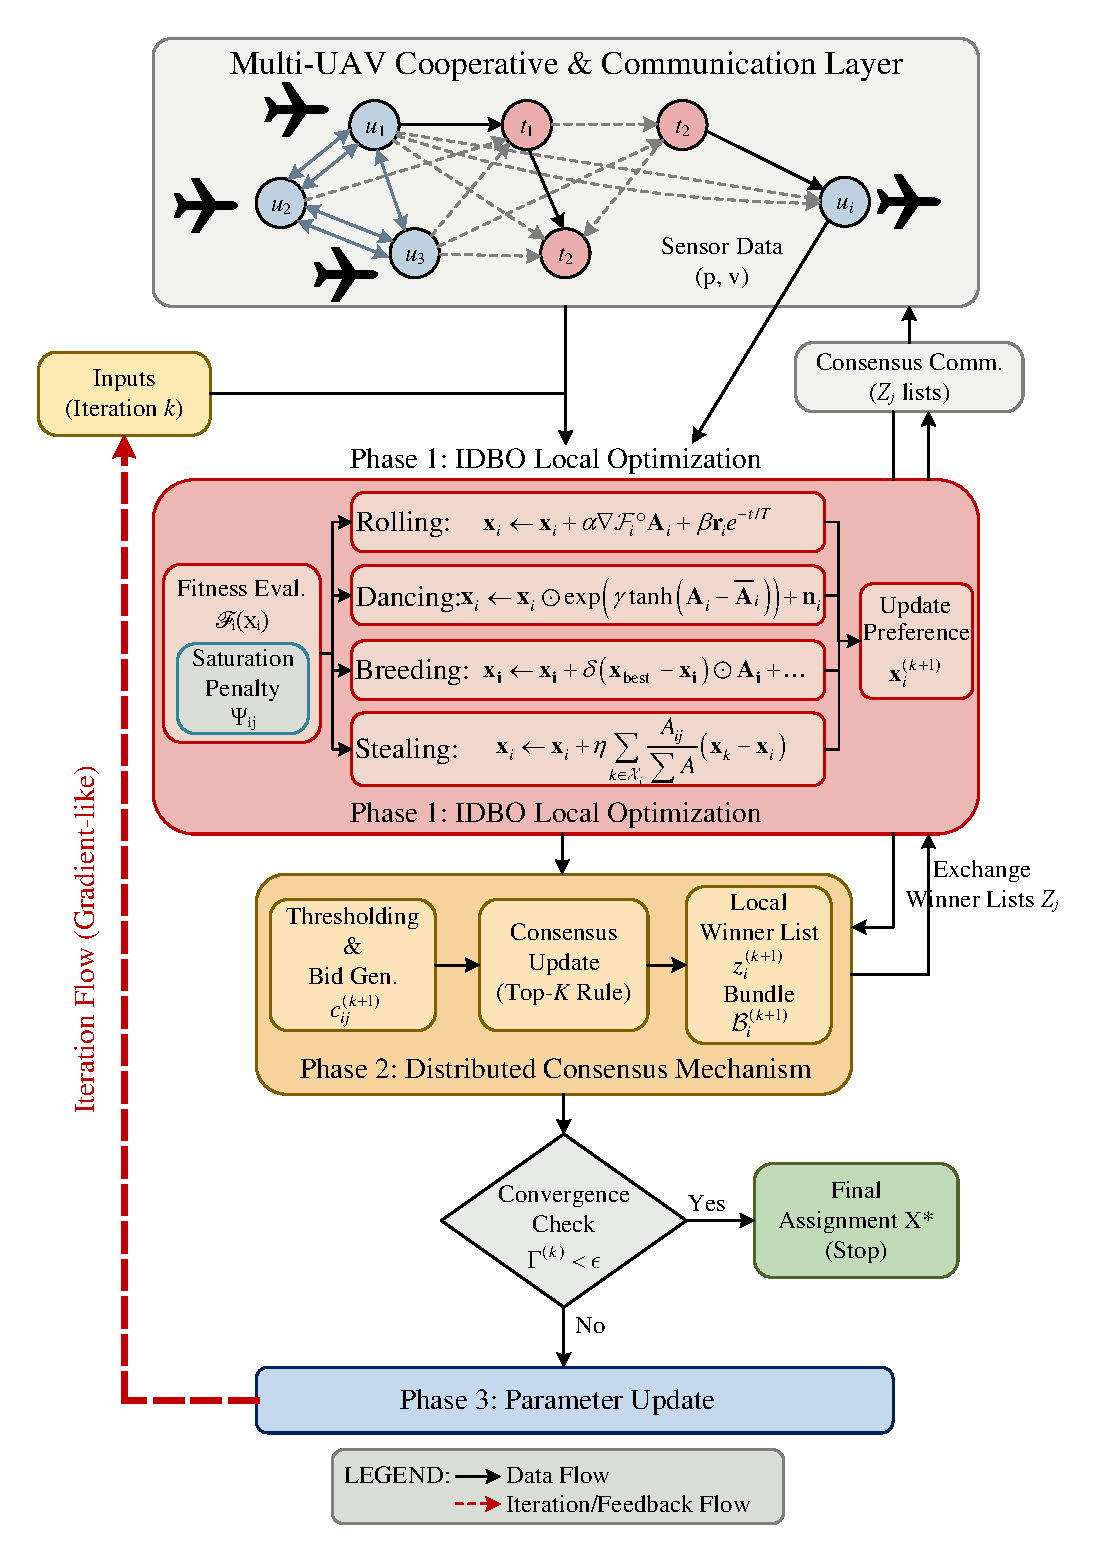
\includegraphics[width=3.2in]{assignment.pdf}
\caption{Flowchart of the distributed consensus-based IDBO algorithm, illustrating the algorithmic iteration flow across local metaheuristic optimization, auction-based consensus, and adversarial information updates.}
\label{fig:idbo_flowchart}
\end{figure}

Here, $\mathcal{H}$ updates adversarial advantages given the consensus assignment and velocity vectors $\mathbf{V}_i$, $\mathbf{V}_T$. Following the iteration flow in Fig.~\ref{fig:idbo_flowchart}, convergence is declared when the swarm-wide assignment disagreement falls below $\epsilon$:

\begin{equation}
\label{eq:convergence}
\Gamma^{(k)} = \frac{1}{M} \sum_{i=1}^{M} \left\| \mathbf{z}_i^{(k)} - \frac{1}{|\mathcal{N}_i|} \sum_{j \in \mathcal{N}_i} \mathbf{z}_j^{(k)} \right\|_0 < \epsilon
\end{equation}
where $\|\cdot\|_0$ counts disagreeing entries and $\epsilon$ is a convergence threshold.

\subsection{Discussion on Convergence and Equilibrium Properties}
\label{subsec:convergence_equilibrium}

The convergence claims in this paper refer to convergence of the distributed assignment
process for a fixed engagement snapshot, rather than a proof of global optimality for the
nonconvex mixed-integer problem in \eqref{eq:optimization_formulation}. The discussion is
based on the following standard conditions: (i) the interceptor and target sets are fixed
during one assignment round; (ii) the communication graph among interceptors is connected and
has bounded message delays; (iii) the feasible assignment set is finite because $X_{ij}$ is
binary and the capacity constraints are finite; and (iv) the local IDBO update adopts elitist
acceptance, i.e., a newly generated preference is retained only when it does not decrease the
local fitness after feasibility projection.

Under these conditions, the local search stage produces a nondecreasing sequence of accepted
fitness values,
\begin{equation}
\label{eq:fitness_monotonic}
\Phi^{(k+1)} \geq \Phi^{(k)}, \quad
\Phi^{(k)}=\sum_{i=1}^{M}\mathcal{F}_i(\mathbf{x}_i^{(k)}),
\end{equation}
until no locally admissible preference update can further improve the aggregate accepted
fitness. Since the feasible binary assignment space is finite, the accepted sequence cannot
increase indefinitely and must eventually reach a fixed point or a finite plateau. The
consensus stage then resolves conflicts by retaining the top-$L_{\max}$ bids for each target.
Because the same winner information is repeatedly exchanged over a connected graph, the
highest bids propagate across the graph within a finite number of communication rounds\DIFdelbegin \DIFdel{bounded by the graph diameter $D$. Thus, after at most $O(ND)$ winner-propagation roundsfor
all targets, all interceptors }\DIFdelend \DIFaddbegin \DIFadd{.
With link delay bounded by \(d_{\max}\), a fixed winner record crosses the
graph within at most \((d_{\max}+1)D\) successful forwarding rounds, where
\(D\) is the graph diameter. With packet loss, the latest timestamped record is
retransmitted, and finite agreement requires every active link to deliver
within a bounded retransmission interval. Thus all interceptors eventually
}\DIFaddend hold the same winner lists, and the disagreement metric
$\Gamma^{(k)}$ in \eqref{eq:convergence} falls below the prescribed tolerance.

\DIFdelbegin \DIFdel{The resulting assignment $\mathbf{X}^{*}$ can be interpreted as an $\epsilon$-approximate
Nash equilibrium of the distributed assignment game induced by the local utilities
$\mathcal{F}_i$. Specifically, after consensus, no interceptor can unilaterally switch to
another feasible target and improve its local utility by more than $\epsilon$ without either
losing the auction for that target or violating the capacity constraint:
}\DIFdelend \DIFaddbegin \DIFadd{After consensus, a local unilateral-deviation diagnostic can be evaluated as
}\DIFaddend \begin{equation}
\label{eq:epsilon_nash}
\mathcal{F}_i(\mathbf{x}_i^{*})
\geq \mathcal{F}_i(\mathbf{x}_i')-\epsilon,\quad
\forall \mathbf{x}_i'\in\mathcal{X}_i,\;\forall i .
\end{equation}
\DIFdelbegin \DIFdel{This equilibrium property is local and assignment-round specific. It ensures consistency and
unilateral stability of the distributed decision, but it does not imply that IDBO always
attains the globally optimal solution }\DIFdelend \DIFaddbegin \DIFadd{When this inequality is verified for the finite feasible alternatives, it
indicates local unilateral stability for that assignment round. Consensus
alone, however, does not prove that the stochastic IDBO search always satisfies
Eq.~}\eqref{eq:epsilon_nash}\DIFadd{, reaches a Nash equilibrium, or attains the global
optimum }\DIFaddend of \eqref{eq:optimization_formulation}. For the
ART-MAPPO guidance stage, convergence is treated empirically because neural policy
optimization is nonconvex; the dual-clip and adaptive KL terms constrain policy update
magnitude and improve training stability, while the observed learning curves in
Section~\ref{subsec:training} validate practical convergence behavior.

The per-UAV per-iteration complexity decomposes as:

\begin{equation}
\label{eq:complexity}
C_{\text{total}} = O(T \cdot P \cdot N^2) + O(N \cdot |\mathcal{N}_i|) + O(N)
\end{equation}
where $T$ is the IDBO iteration count, $P = O(N)$ the population size, and $|\mathcal{N}_i|$ the neighborhood size. The three terms account for optimization, consensus communication, and advantage update, respectively. Communication cost is $O(N \cdot |\mathcal{N}_i|)$ and memory is $O(P \cdot N + N)$ per UAV.

For reproducibility, the complete target-assignment procedure is summarized in
Algorithm~\ref{alg:idbo}.

\begin{algorithm}[!t]
\caption{Distributed Consensus-Based IDBO Target Assignment}
\label{alg:idbo}
\footnotesize
\begin{algorithmic}[1]
\REQUIRE Interceptor set $\mathcal{U}$, target set $\mathcal{T}$, pairwise weights $P_{ij}$,
advantage estimates $A_{ij}$, neighbor sets $\mathcal{N}_i$, capacity $L_{\max}$, threshold
$\epsilon$, maximum iteration $K_{\max}$
\ENSURE Consensus assignment matrix $\mathbf{X}^{*}$
\STATE Initialize each preference vector $\mathbf{x}_i$, bundle $\mathcal{B}_i$, bid vector
$\mathbf{c}_i$, winner list $\mathbf{z}_i$, and timestamp vector $\mathbf{y}_i$
\FOR{$k=0$ to $K_{\max}-1$}
    \FOR{each interceptor $u_i\in\mathcal{U}$}
        \STATE Compute local fitness $\mathcal{F}_i(\mathbf{x}_i)$ using $P_{ij}$,
        $A_{ij}$, and the saturation penalty $\Psi_{ij}$
        \STATE Update $\mathbf{x}_i$ by the IDBO rolling, dancing, breeding, and stealing
        operators in Eqs.~\eqref{eq:rolling_update}--\eqref{eq:stealing_update}
        \STATE Binarize preferences into candidate assignments using
        Eq.~\eqref{eq:thresholding}
        \STATE Compute bids $c_{ij}$ for candidate targets using Eq.~\eqref{eq:bid_formulation}
        \STATE Broadcast $\{\mathcal{B}_i,\mathbf{c}_i,\mathbf{z}_i,\mathbf{y}_i\}$ to
        neighbors in $\mathcal{N}_i$
        \STATE Merge neighbor bids and retain the top-$L_{\max}$ winners for each target
        according to Eq.~\eqref{eq:cbba_update}
        \STATE Update $\mathcal{B}_i$, $\mathbf{z}_i$, and the local assignment row
        $\mathbf{X}_{i,:}^{(k+1)}$
        \STATE Update the advantage vector $\mathbf{A}_i^{(k+1)}$ from the current consensus
        assignment and velocity information
    \ENDFOR
    \STATE Compute swarm disagreement $\Gamma^{(k+1)}$ using Eq.~\eqref{eq:convergence}
    \IF{$\Gamma^{(k+1)}<\epsilon$}
        \STATE \textbf{break}
    \ENDIF
\ENDFOR
\STATE \textbf{return} $\mathbf{X}^{*}\leftarrow\mathbf{X}^{(k+1)}$
\end{algorithmic}
\end{algorithm}













%% ===========================================================
\section{ART-MAPPO: Attention-Residual and Trust-Aware MAPPO for Cooperative Swarm Interception}
\label{sec:cooperative_algorithm}

Building on the distributed consensus-based IDBO target assignment, we propose the Attention-Residual and Trust-aware MAPPO (ART-MAPPO) algorithm for the cooperative guidance of defending UAV swarms under the Centralized Training with Decentralized Execution (CTDE) paradigm. ART-MAPPO augments the standard MAPPO framework with three synergistic modules: a kinematics-aware attention-residual network for extracting cross-coupled engagement features, a trust-modulated exploration mechanism for discovering cooperative tactics within the safe flight envelope, and a dual-clip PPO with adaptive KL penalty for constraining guidance command variations against actuator saturation.

\subsection{Enhanced Situational Awareness via Attention-Residual Network}
\label{subsec:attention_residual}

The highly dynamic nature of swarm interception requires interceptors to process complex, coupled kinematic states. The network therefore first maps the compact physical observation into a latent representation where nonlinear engagement patterns can be learned more easily. Let $\mathbf{o}_i^{(t)} \in \mathbb{R}^{n_o}$ denote the observation vector for interceptor $i$ at time step $t$, as defined in Section~\ref{subsec:state_reward}. A base feature encoder $f_{\mathrm{enc}}$, comprising a two-layer MLP with hidden dimension $d_{\mathrm{enc}}$ and Layer Normalization, projects the raw observation into a high-dimensional latent space:
\begin{equation}
\label{eq:encoder}
\begin{split}
\mathbf{h}^{(0)} =& \operatorname{LN}\Bigl(\operatorname{ReLU}\bigl(\mathbf{o}_i^{(t)}\mathbf{W}_{\mathrm{enc}}^{(1)} + \mathbf{b}_{\mathrm{enc}}^{(1)}\bigr) \\
&\cdot \mathbf{W}_{\mathrm{enc}}^{(2)} + \mathbf{b}_{\mathrm{enc}}^{(2)}\Bigr) \in \mathbb{R}^{d}
\end{split}
\end{equation}
where $\mathbf{W}_{\mathrm{enc}}^{(1)} \in \mathbb{R}^{n_o \times d_{\mathrm{enc}}}$ and $\mathbf{W}_{\mathrm{enc}}^{(2)} \in \mathbb{R}^{d_{\mathrm{enc}} \times d}$ are learnable projection matrices.

\emph{1) Kinematics-Aware Multi-Head Attention:} To capture the nonlinear spatio-temporal coupling among engagement variables (e.g., the interdependence between LOS rate $\dot{q}$ and time-to-go synchronization), we reshape $\mathbf{h}^{(0)}$ into a sequence of $n_o$ feature tokens $\mathbf{H}^{(0)} \in \mathbb{R}^{n_o \times (d/n_o)}$ and apply multi-head self-attention. For each head $j \in \{1, \dots, H\}$, the query, key, and value projections are:
\begin{equation}
\label{eq:qkv}
\mathbf{Q}_j = \mathbf{H}^{(0)}\mathbf{W}_j^{Q}, \quad \mathbf{K}_j = \mathbf{H}^{(0)}\mathbf{W}_j^{K}, \quad \mathbf{V}_j = \mathbf{H}^{(0)}\mathbf{W}_j^{V}
\end{equation}
where $\mathbf{W}_j^{Q}, \mathbf{W}_j^{K} \in \mathbb{R}^{(d/n_o) \times d_k}$ and $\mathbf{W}_j^{V} \in \mathbb{R}^{(d/n_o) \times d_v}$, with $d_k = d_v = d/H$. The scaled dot-product attention for head $j$, incorporating an observability mask $\mathbf{M} \in \mathbb{R}^{n_o \times n_o}$, is:
\begin{align}
\mathbf{A}_j &= \mathrm{softmax}\!\left(\frac{\mathbf{Q}_j\mathbf{K}_j^\top}{\sqrt{d_k}} + \mathbf{M}\right) \in \mathbb{R}^{n_o \times n_o} \label{eq:attention} \\
\mathrm{head}_j &= \mathbf{A}_j\mathbf{V}_j \in \mathbb{R}^{n_o \times d_v} \nonumber
\end{align}
where $M_{u,v} = -\infty$ isolates unobservable kinematic channels (e.g., LOS rate during sensor blanking) and $M_{u,v} = 0$ permits information flow. The multi-head outputs are concatenated, projected, and added back via a residual shortcut:
\begin{equation}
\label{eq:mha_out}
\begin{split}
\mathbf{h}_{\mathrm{attn}} =& \mathbf{h}^{(0)} + \mathrm{Dropout}_{p}\Bigl(\operatorname{Flatten}\bigl( \\
&\left[\mathrm{head}_1 \| \cdots \| \mathrm{head}_H\right]\bigr) \mathbf{W}^{O}\Bigr)
\end{split}
\end{equation}
where $\mathbf{W}^{O} \in \mathbb{R}^{d \times d}$ is the output projection and $\operatorname{Flatten}(\cdot)$ reshapes the token sequence back to $\mathbb{R}^d$. The residual connection ensures that primitive flight-state components propagate losslessly to downstream layers.

\emph{2) Residual Block with Layer Normalization:} To deepen the nonlinear representational capacity without gradient vanishing---a critical issue when extreme overload commands produce large-magnitude gradients---a stack of $L$ residual blocks follows the attention module. For the $\ell$-th block ($\ell \in \{1, \dots, L\}$) with input $\mathbf{h}^{(\ell)}$ (where $\mathbf{h}^{(1)} = \mathbf{h}_{\mathrm{attn}}$), the forward pass is:
\begin{align}
\mathbf{z}_1^{(\ell)} &= \operatorname{ReLU} \left( \operatorname{LN}_1^{(\ell)} \left( \mathbf{h}^{(\ell)}\mathbf{W}_1^{(\ell)} + \mathbf{b}_1^{(\ell)} \right) \right) \label{eq:res_block_inner1} \\
\mathbf{z}_2^{(\ell)} &= \operatorname{LN}_2^{(\ell)} \left( \mathbf{z}_1^{(\ell)}\mathbf{W}_2^{(\ell)} + \mathbf{b}_2^{(\ell)} \right) \label{eq:res_block_inner2} \\
\mathbf{h}^{(\ell+1)} &= \operatorname{ReLU} \left( \mathbf{z}_2^{(\ell)} + \mathbf{h}^{(\ell)} \right) \label{eq:res_block_out}
\end{align}
where $\mathbf{W}_1^{(\ell)}, \mathbf{W}_2^{(\ell)} \in \mathbb{R}^{d \times d}$ are orthogonally initialized. The identity shortcut yields the Jacobian:
\begin{equation}
\label{eq:jacobian}
\begin{split}
\frac{\partial \mathbf{h}^{(\ell+1)}}{\partial \mathbf{h}^{(\ell)}} =& \operatorname{diag}\!\left(\mathbb{I}\!\left[\mathbf{z}_2^{(\ell)} + \mathbf{h}^{(\ell)} > \mathbf{0}\right]\right) \\
&\cdot \left(\mathbf{I} + \frac{\partial \mathbf{z}_2^{(\ell)}}{\partial \mathbf{h}^{(\ell)}}\right)
\end{split}
\end{equation}
Since the ReLU gate preserves the identity component on active units, gradient norms satisfy $\left\|\frac{\partial \mathbf{h}^{(\ell+1)}}{\partial \mathbf{h}^{(\ell)}}\right\| \geq \left\|\operatorname{diag}(\mathbb{I}[\cdot])\right\| > 0$, preventing vanishing gradients across $L$ blocks.

\emph{3) End-to-End Guidance Command Generation:} The refined feature $\mathbf{h}^{(L+1)}$ is fed into a GRU cell to integrate temporal engagement history:
\begin{equation}
\label{eq:gru}
\mathbf{c}_t = \operatorname{GRU}\!\left(\mathbf{h}^{(L+1)},\, \mathbf{c}_{t-1};\, \mathbf{W}_{\mathrm{GRU}}\right), \quad \mathbf{c}_t \in \mathbb{R}^{d_{\mathrm{rnn}}}
\end{equation}
where $\mathbf{W}_{\mathrm{GRU}}$ denotes the GRU parameters and $\mathbf{c}_{t-1}$ is the hidden state from the previous guidance step. The actor network then parameterizes a diagonal Gaussian over the continuous overload action space:
\DIFdelbegin %DIFDELCMD < \begin{equation}
%DIFDELCMD < \label{eq:actor_dist}
%DIFDELCMD < \begin{split}
%DIFDELCMD < \pi_{\theta_i}\!\left(a_i \mid \mathbf{o}_i^{(t)}\right) &= \mathcal{N}\!\left(\boldsymbol{\mu}_{\theta_i}(\mathbf{c}_t),\; \operatorname{diag}\!\left(\boldsymbol{\sigma}_{\theta_i}^2(\mathbf{c}_t)\right)\right) \\
%DIFDELCMD < a_i &= [n_{x_i},\, n_{y_i}]^\top \in \mathcal{A}
%DIFDELCMD < \end{split}
%DIFDELCMD < \end{equation}%%%
\DIFdelend \DIFaddbegin \begin{equation}
\label{eq:actor_dist}
\begin{split}
\pi_{\theta_i}\!\left(a_i \mid \mathbf{o}_i^{(t)}\right) &= \mathcal{N}\!\left(\boldsymbol{\mu}_{\theta_i}(\mathbf{c}_t),\; \operatorname{diag}\!\left(\boldsymbol{\sigma}_{\theta_i}^2(\mathbf{c}_t)\right)\right) \\
a_i &= [n_{x_i},\, n_{y_i},\,n_{z_i}]^\top \in \mathcal{A}
\end{split}
\end{equation}\DIFaddend 
where \DIFdelbegin \DIFdel{$\boldsymbol{\mu}_{\theta_i}, \boldsymbol{\sigma}_{\theta_i}^2: \mathbb{R}^{d_{\mathrm{rnn}}} \to \mathbb{R}^2$ }\DIFdelend \DIFaddbegin \DIFadd{$\boldsymbol{\mu}_{\theta_i}, \boldsymbol{\sigma}_{\theta_i}^2:
\mathbb{R}^{d_{\mathrm{rnn}}} \to \mathbb{R}^3$ }\DIFaddend are linear output heads \DIFaddbegin \DIFadd{and
\(\mathcal A=[-0.1,1]\times[-1,1]\times[-1,1]\)}\DIFaddend . The action is clipped to
\DIFdelbegin \DIFdel{the feasible envelope $\mathcal{A}$ }\DIFdelend \DIFaddbegin \DIFadd{this feasible three-dimensional envelope }\DIFaddend after sampling. Concurrently, the
centralized critic shares the same attention-residual backbone but receives the
concatenated global state:
\begin{equation}
\label{eq:critic_input}
s_t = \left[\mathbf{o}_1^{(t)} \| \mathbf{o}_2^{(t)} \| \cdots \| \mathbf{o}_N^{(t)}\right] \in \mathbb{R}^{N \cdot n_o}
\end{equation}
to produce the state-value estimate $V_\phi(s_t) \in \mathbb{R}$, enabling centralized advantage computation during training while each actor executes independently from local observations $\mathbf{o}_i^{(t)}$ at deployment.

\subsection{Trust-Modulated Tactical Exploration}
\label{subsec:trust_exploration}

Based on the \DIFdelbegin \DIFdel{high-fidelity }\DIFdelend \DIFaddbegin \DIFadd{coupled kinematic }\DIFaddend features extracted by the
attention-residual backbone, we introduce a trust-based mechanism to dynamically
modulate the exploration policy. This mechanism mathematically balances the
exploitation of known guidance laws against the discovery of complex
cooperative tactics (e.g., flanking or simultaneous impact).

\emph{1) Trust Evolution:} Trust can be interpreted as a smoothed memory of how reliably an interceptor has performed relative to the swarm average. Let $R_i^{(k)} = \sum_{t=0}^{T} \gamma_{\mathrm{RL}}^t r_i^{(t)}$ be the discounted cumulative return of interceptor $i$ in episode $k$, where $\gamma_{\mathrm{RL}} \in (0,1)$ is the RL discount factor (distinct from the heading angle $\gamma_{D_i}$) and $T$ is the episode horizon. The swarm-level running statistics are maintained as exponential moving averages:
\begin{align}
\mu_R &\leftarrow (1-\rho)\,\mu_R + \rho\,\frac{1}{N}\sum_{i=1}^{N} R_i^{(k)} \label{eq:running_stats_mu} \\
\sigma_R^2 &\leftarrow (1-\rho)\,\sigma_R^2 + \rho\,\frac{1}{N}\sum_{i=1}^{N}\!\left(R_i^{(k)} - \mu_R\right)^2 \label{eq:running_stats_sigma}
\end{align}
where $\rho \in (0,1)$ is the statistics update rate. The normalized relative performance below measures whether interceptor $i$ is performing above or below the recent swarm baseline, making the trust update insensitive to the absolute reward scale:
\begin{equation}
\label{eq:trust_normalized}
\tilde{R}_i^{(k)} = \frac{R_i^{(k)} - \mu_R}{\sqrt{\sigma_R^2 + \epsilon_0}}
\end{equation}
where $\epsilon_0 > 0$ is a numerical stabilizing constant. The trust level $\mathcal{T}_i^{(k)} \in (0,1)$ evolves via first-order exponential smoothing with a sigmoid activation:
\begin{equation}
\label{eq:trust_evolution}
\mathcal{T}_i^{(k+1)} = (1-\alpha_T)\,\mathcal{T}_i^{(k)} + \alpha_T\,\sigma\!\left(\tau_T \tilde{R}_i^{(k)}\right)
\end{equation}
where $\sigma(x) = 1/(1+e^{-x})$, $\alpha_T \in (0,1)$ is the trust update rate and $\tau_T > 0$ is the temperature parameter controlling the sensitivity of trust to performance deviations. \DIFdelbegin \DIFdel{When $R_i^{(k)} > \mu_R$,
the sigmoid output exceeds 0.5, driving $\mathcal{T}_i$ upward and reducing exploration; conversely, below-average performance lowers $\mathcal{T}_i$ and amplifies exploration}\DIFdelend \DIFaddbegin \DIFadd{Equivalently,
}\begin{equation}
\label{eq:trust_increment}
\mathcal T_i^{(k+1)}-\mathcal T_i^{(k)}
=\alpha_T\!\left[
\sigma(\tau_T\widetilde R_i^{(k)})-\mathcal T_i^{(k)}\right].
\end{equation}
\DIFadd{Thus, above-average performance raises the instantaneous trust target, but
trust itself increases only when that target exceeds its current value; it can
also decrease when recent performance deteriorates. For fixed normalized
return, Eq.~}\eqref{eq:trust_evolution} \DIFadd{is a contraction with factor
\(1-\alpha_T\), which explains the smoothing behavior without assuming
monotonic trust growth}\DIFaddend .

\emph{2) Blended Exploration Policy:} The exploration policy links trust to action selection. High-trust interceptors mainly exploit the learned policy, whereas low-trust interceptors are more likely to try structured guidance actions that expose useful maneuvering experience. The final action for interceptor $i$ is drawn from a two-component mixture: with probability $1-\beta(\mathcal{T}_i)$ from the learned policy, and with probability $\beta(\mathcal{T}_i)$ from a structured heuristic distribution, i.e.,
\begin{equation}
\label{eq:exploration_policy}
a_i \sim \begin{cases} \pi_{\theta_i}(\cdot \mid \mathbf{o}_i^{(t)}) & \text{with prob. } 1 - \beta(\mathcal{T}_i) \\ \pi_{\mathrm{guided}}^{i}(\cdot \mid \mathbf{o}_i^{(t)}) & \text{with prob. } \beta(\mathcal{T}_i) \end{cases}
\end{equation}
where the modulation factor $\beta(\mathcal{T}_i) = 1 - \mathcal{T}_i \in (0,1)$ is monotonically decreasing in trust. The heuristic distribution $\pi_{\mathrm{guided}}^{i}$ is a discrete mixture over three tactically informative actions within the feasible command space
\DIFdelbegin \DIFdel{$\mathcal{A} = [n_{x}^{\min}, n_{x}^{\max}] \times [n_{y}^{\min}, n_{y}^{\max}]$}\DIFdelend \DIFaddbegin \DIFadd{\(\mathcal{A}=[n_x^{\min},n_x^{\max}]\times
[n_y^{\min},n_y^{\max}]\times[n_z^{\min},n_z^{\max}]\)}\DIFaddend :
\begin{equation}
\label{eq:guided}
\begin{split}
\pi_{\mathrm{guided}}^{i}(a_i \mid \mathbf{o}_i^{(t)}) =& \omega_1\,\delta(a_i - a_{\mathrm{opt}}) + \omega_2\,\delta(a_i - a_{\mathrm{probe}}) \\
&+ \omega_3\,\mathcal{U}(\mathcal{A}), \quad \sum_{k=1}^3\omega_k=1
\end{split}
\end{equation}
Here, $a_{\mathrm{opt}} = \arg\max_{a \in \mathcal{A}} Q_\phi(\mathbf{o}_i^{(t)}, a)$ mimics the classical proportional navigation command for exploitation, $a_{\mathrm{probe}} = \arg\min_{a \in \mathcal{A}} Q_\phi(\mathbf{o}_i^{(t)}, a)$ deliberately executes extreme boundary maneuvers to probe the aerodynamic envelope, and $\mathcal{U}(\mathcal{A})$ maintains stochastic coverage of the remaining action space. The expected action under the full mixture policy is:
\begin{equation}
\label{eq:expected_action}
\begin{split}
\mathbb{E}[a_i] =& \bigl(1-\beta(\mathcal{T}_i)\bigr)\,\boldsymbol{\mu}_{\theta_i}(\mathbf{c}_t) \\
&+ \beta(\mathcal{T}_i)\,\bigl(\omega_1\,a_{\mathrm{opt}} + \omega_2\,a_{\mathrm{probe}} + \omega_3\,\bar{a}_{\mathcal{A}}\bigr)
\end{split}
\end{equation}
where
\DIFdelbegin \DIFdel{$\bar{a}_{\mathcal{A}} = \frac{1}{2}[n_x^{\min}+n_x^{\max},\; n_y^{\min}+n_y^{\max}]^\top$ }\DIFdelend \DIFaddbegin \DIFadd{\(\bar{a}_{\mathcal{A}}=\frac{1}{2}
[n_x^{\min}+n_x^{\max},\,n_y^{\min}+n_y^{\max},\,
n_z^{\min}+n_z^{\max}]^\top\) }\DIFaddend is the centroid of \DIFdelbegin \DIFdel{$\mathcal{A}$}\DIFdelend \DIFaddbegin \DIFadd{\(\mathcal{A}\)}\DIFaddend .

\subsection{Robust Optimization via Dual-Clip and Adaptive KL}
\label{subsec:dual_clip_kl}

Aggressive exploration inherently induces substantial variations in the importance-sampling ratio $r_t(\theta) = \pi_\theta(a_t \mid o_t) / \pi_{\theta_{\mathrm{old}}}(a_t \mid o_t)$, leading to oscillatory terminal overload commands $n_{y_i}$ that can severely compromise flight stability. We stabilize policy gradient optimization using a dual-clip surrogate objective combined with an adaptive KL divergence penalty.

\emph{1) Generalized Advantage Estimation:} The advantage $\hat{A}_t$ is computed via GAE with discount $\gamma_{\mathrm{RL}}$ and trace-decay $\lambda_{\mathrm{GAE}} \in [0,1]$:
\begin{align}
\hat{A}_t &= \sum_{l=0}^{T-t-1} (\gamma_{\mathrm{RL}}\lambda_{\mathrm{GAE}})^l \delta_{t+l} \label{eq:gae_A} \\
\delta_t &= r_i^{(t)} + \gamma_{\mathrm{RL}} V_\phi(s_{t+1}) - V_\phi(s_t) \label{eq:gae_delta}
\end{align}
where $\delta_t$ is the TD residual. The corresponding value target is $\hat{V}_t^{\mathrm{targ}} = \hat{A}_t + V_\phi(s_t)$.

\emph{2) Dual-Clip PPO Objective:} Policy updates are most dangerous when a poor action receives a large probability-ratio correction, because this can create abrupt overload changes. The standard clipped surrogate is:
\begin{equation}
\label{eq:standard_clip}
\begin{split}
L^{\mathrm{CLIP}}(\theta) = \min \Bigl( &r_t(\theta)\hat{A}_t, \\
&\operatorname{clip}\!\left(r_t(\theta), 1-\epsilon, 1+\epsilon\right)\hat{A}_t \Bigr)
\end{split}
\end{equation}
where $\epsilon \in (0,1)$ is the clipping threshold. When $\hat{A}_t < 0$, the standard clip permits $r_t(\theta) \to \infty$, causing catastrophic over-correction of overload commands. The Dual-Clip objective addresses this by introducing a floor $c > 1+\epsilon$ applied only when $\hat{A}_t < 0$:
\begin{equation}
\label{eq:dual_clip_final}
J^{\mathrm{DC}}(\theta) = \mathbb{E}_{t} \left[
\begin{cases}
\max\!\left( L^{\mathrm{CLIP}}(\theta),\; c\,\hat{A}_t \right) & \hat{A}_t < 0 \\[4pt]
L^{\mathrm{CLIP}}(\theta) & \hat{A}_t \geq 0
\end{cases}
\right]
\end{equation}
When $\hat{A}_t < 0$, the $\max$ with $c\,\hat{A}_t$ \DIFdelbegin \DIFdel{bounds $r_t(\theta) \leq c$, preventing the
policy from over-penalizing actions that only marginally degrade performance}\DIFdelend \DIFaddbegin \DIFadd{lower-bounds the
sample surrogate contribution and prevents an excessively large negative
update from dominating the mini-batch}\DIFaddend . When $\hat{A}_t \geq 0$, the standard
pessimistic clip \DIFdelbegin \DIFdel{suffices. The effective constraint on $r_t(\theta)$ under the dual-clip is therefore:
}%DIFDELCMD < \begin{equation}
%DIFDELCMD < \label{eq:rt_bound}
%DIFDELCMD < r_t(\theta) \in \begin{cases} \left[\frac{1}{c},\; c\right] & \hat{A}_t < 0 \\[4pt] \left[1-\epsilon,\; 1+\epsilon\right] & \hat{A}_t \geq 0 \end{cases}
%DIFDELCMD < \end{equation}
%DIFDELCMD < %%%
\DIFdelend \DIFaddbegin \DIFadd{is retained. Dual clipping therefore regularizes the
surrogate objective; it does not impose a hard pointwise interval on every
realized probability ratio \(r_t(\theta)\).
}\DIFaddend 

\emph{3) Adaptive KL Regularization:} The KL term acts as an update-speed monitor: when the new policy moves too far from the old policy, subsequent updates are damped; when the policy changes too little, optimization is allowed to proceed more freely. To continuously constrain policy deviation between updates, the KL divergence is approximated as:
\begin{equation}
\label{eq:kl_approx}
\begin{split}
\hat{D}_{\mathrm{KL}}\!\left(\pi_{\theta_{\mathrm{old}}} \| \pi_\theta\right) &= \mathbb{E}_t\!\left[\log\frac{\pi_{\theta_{\mathrm{old}}}(a_t \mid o_t)}{\pi_\theta(a_t \mid o_t)}\right] \\
&= \mathbb{E}_t\!\left[\log\pi_{\theta_{\mathrm{old}}}(a_t \mid o_t) - \log\pi_\theta(a_t \mid o_t)\right]
\end{split}
\end{equation}
The penalty coefficient $\beta_{\mathrm{KL}}$ is updated after each training epoch $k$ via:
\begin{equation}
\label{eq:kl_adapt}
\beta_{\mathrm{KL}}^{(k+1)} =
\begin{cases}
\min\!\left(1.5\,\beta_{\mathrm{KL}}^{(k)},\; \beta_{\max}\right), & \hat{D}_{\mathrm{KL}} > 2\,\delta_{\mathrm{targ}} \\[6pt]
\max\!\left(0.9\,\beta_{\mathrm{KL}}^{(k)},\; \beta_{\min}\right), & \hat{D}_{\mathrm{KL}} < 0.5\,\delta_{\mathrm{targ}} \\[6pt]
\beta_{\mathrm{KL}}^{(k)}, & \text{otherwise}
\end{cases}
\end{equation}
where $\delta_{\mathrm{targ}}$ is the target KL constraint, and $\beta_{\max}=10$, $\beta_{\min}=10^{-4}$ prevent the regularization from dominating or vanishing. When $\hat{D}_{\mathrm{KL}} > 2\delta_{\mathrm{targ}}$, the overload commands have shifted too aggressively between updates, risking structural load-factor exceedance; the $1.5\times$ increase dampens subsequent updates. When $\hat{D}_{\mathrm{KL}} < 0.5\delta_{\mathrm{targ}}$, the $0.9\times$ decay permits finer trajectory refinement.

\emph{4) Overall Loss Formulation:} The critic value loss over a mini-batch of size $B$ is:
\begin{equation}
\label{eq:value_loss}
L_V(\phi) = \frac{1}{B}\sum_{t=1}^{B} \left(V_\phi(s_t) - \hat{V}_t^{\mathrm{targ}}\right)^2
\end{equation}
Combining the dual-clip surrogate, adaptive KL penalty, value loss, and policy entropy bonus $S[\pi_\theta] = -\mathbb{E}_t[\log\pi_\theta(a_t \mid o_t)]$, the unified loss minimized by AdamW with cosine annealing is:
\begin{equation}
\label{eq:total_loss}
\mathcal{L}(\theta,\phi) = - J^{\mathrm{DC}}(\theta) + \beta_{\mathrm{KL}}\,\hat{D}_{\mathrm{KL}} + c_v\,L_V(\phi) - c_e\,S[\pi_\theta]
\end{equation}
where $c_v > 0$ and $c_e > 0$ are the value and entropy weighting coefficients. The learning rate follows a cosine annealing schedule $\eta(k) = \eta_{\min} + \frac{1}{2}(\eta_0 - \eta_{\min})(1 + \cos(\pi k / K))$, facilitating coarse trajectory optimization early in training and fine-grained terminal-guidance refinement in later epochs.

\DIFaddbegin \DIFadd{Dual clipping, adaptive KL coefficient updates, critic evaluation, and trust
statistics are training operations. During deterministic deployment, each UAV
evaluates the attention-residual encoder, GRU state update, and actor mean from
its local observation; no online dual-clip or KL optimization loop is added to
the guidance command path.
}

\DIFaddend The complete ART-MAPPO workflow, integrating all three modules described above, is illustrated in Fig.~\ref{fig:algorithm_flow}.

\begin{figure*}[!t]
\centering
\DIFdelbeginFL %DIFDELCMD < 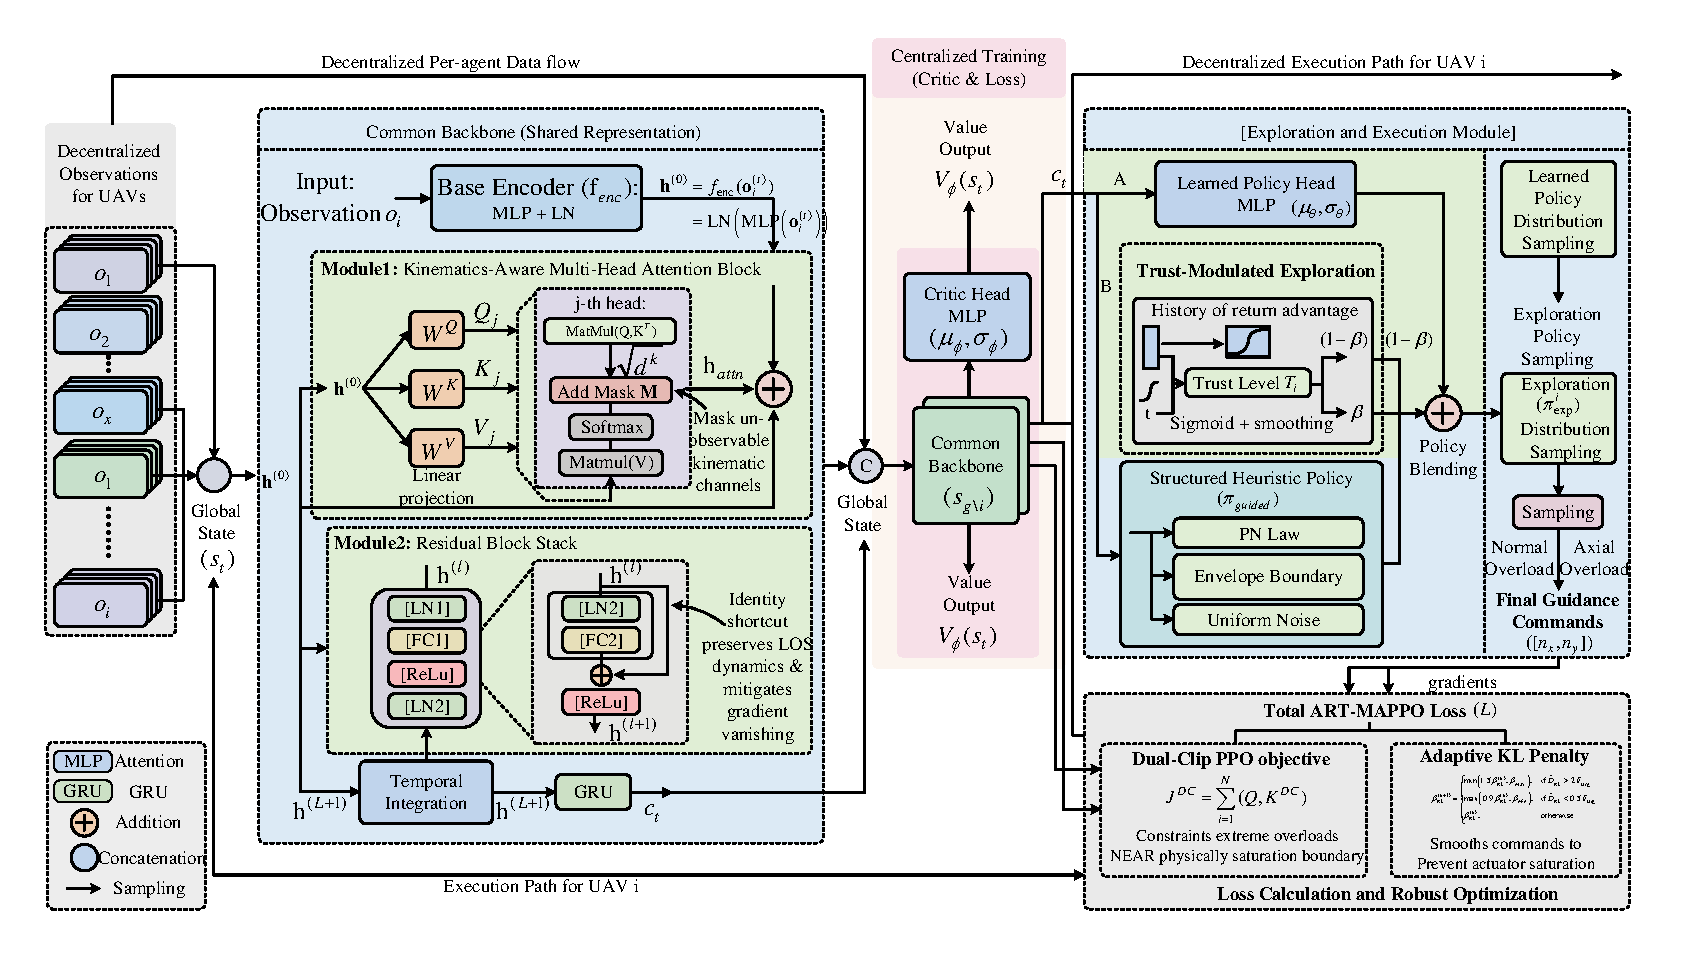
\includegraphics[width=7.3in]{rlsuanfa.pdf}
%DIFDELCMD < %%%
\DIFdelendFL \DIFaddbeginFL 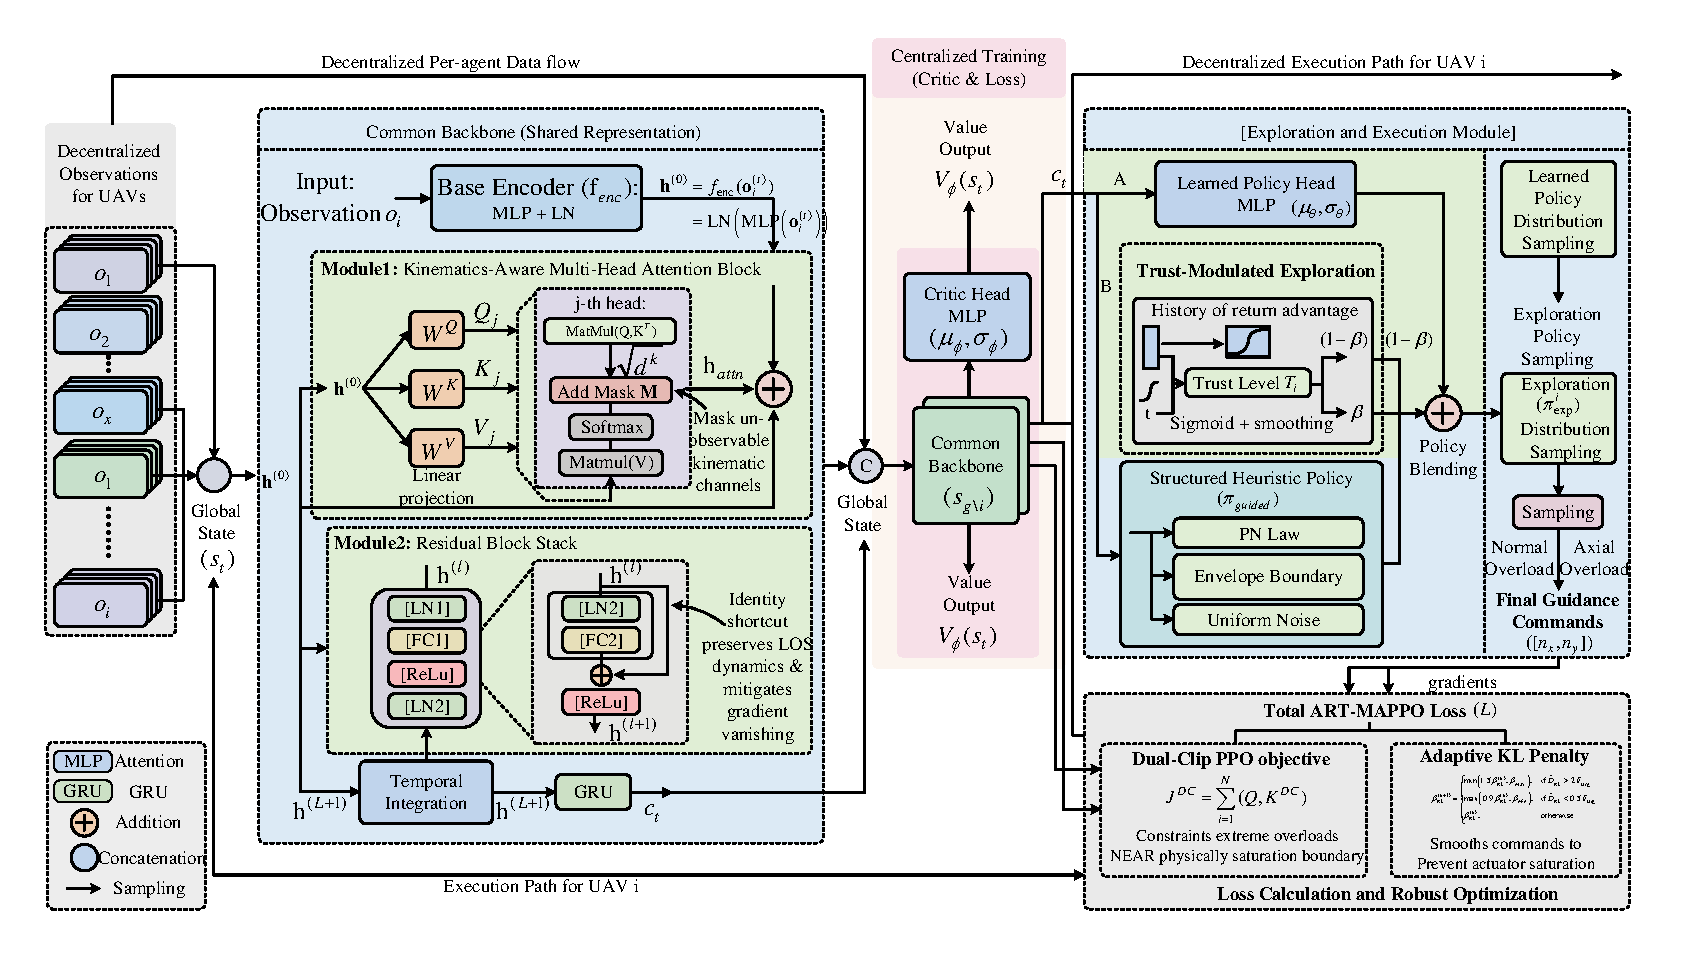
\includegraphics[width=7.1in]{rlsuanfa.pdf}
\DIFaddendFL \caption{Overall workflow of the ART-MAPPO algorithm for cooperative swarm interception, showing the interaction among the attention-residual network, trust-modulated exploration, and dual-clip adaptive KL optimization.}
\label{fig:algorithm_flow}
\end{figure*}

\subsection{State Representation and Reward Design}
\label{subsec:state_reward}

\emph{1) Observation Space:} The \DIFdelbegin \DIFdel{observation vector for interceptor $i$ at time step $t$ is designed to capture the essential kinematic quantities for guidance and coordination:
}%DIFDELCMD < \begin{equation}
%DIFDELCMD < \label{eq:observation_space}
%DIFDELCMD < \mathbf{o}_i^{(t)} = \left[o_i^{(t),1},\; o_i^{(t),2},\; o_i^{(t),3},\; o_i^{(t),4}\right]^\top \in \mathbb{R}^{n_o},\quad n_o = 4
%DIFDELCMD < \end{equation}
%DIFDELCMD < %%%
\DIFdel{The four components are defined as:
%DIF <  \begin{align}
%DIF <  o_i^{(t),1} &= \begin{cases} \dfrac{V_i \dot{q}_t}{g}, & |\dot{q}_t - \dot{q}_{t-1}| \leq \Delta\dot{q}_{\max} \\[6pt] \dfrac{V_i \dot{q}_{t-1}}{g}, & |\dot{q}_t - \dot{q}_{t-1}| > \Delta\dot{q}_{\max} \end{cases} \label{eq:o1} \\[6pt]
%DIF <  o_i^{(t),2} &= \gamma_{D_i} - q_i \label{eq:o2} \\[4pt]
%DIF <  o_i^{(t),3} &= \left(n_{x_i}^2 + n_{y_i}^2\right) \cdot \Delta t \label{eq:o3} \\[4pt]
%DIF <  o_i^{(t),4} &= \frac{r_i}{\min_{j \in \mathcal{G}_i} t_{go_j}} - V_i \label{eq:o4}
%DIF <  \end{align}
}%DIFDELCMD < \begin{align}
%DIFDELCMD < o_i^{(t),1} &=
%DIFDELCMD < \begin{cases}
%DIFDELCMD < \dfrac{V_i \dot{q}_i^{(t)}}{g}, &
%DIFDELCMD < \left|\dot{q}_i^{(t)} - \dot{q}_i^{(t-1)}\right| \leq \Delta \dot{q}_{\max}
%DIFDELCMD < \\[6pt]
%DIFDELCMD < \dfrac{V_i \dot{q}_i^{(t-1)}}{g}, &
%DIFDELCMD < \left|\dot{q}_i^{(t)} - \dot{q}_i^{(t-1)}\right| > \Delta \dot{q}_{\max}
%DIFDELCMD < \end{cases}
%DIFDELCMD < \label{eq:o1}
%DIFDELCMD < \\[6pt]
%DIFDELCMD < o_i^{(t),2} &= \gamma_{D_i} - q_i
%DIFDELCMD < \label{eq:o2}
%DIFDELCMD < \\[4pt]
%DIFDELCMD < o_i^{(t),3} &= \left(n_{x_i}^2 + n_{y_i}^2\right)\cdot \Delta t
%DIFDELCMD < \label{eq:o3}
%DIFDELCMD < \\[4pt]
%DIFDELCMD < o_i^{(t),4} &= \frac{r_i}{\min_{j \in \mathcal{G}_i} t_{go_j}} - V_i
%DIFDELCMD < \label{eq:o4}
%DIFDELCMD < \end{align}
%DIFDELCMD < %%%
\DIFdel{where $\Delta\dot{q}_{\max} = 0.03$~rad/s is the LOS-rate noise threshold,
$\mathcal{G}_i$ denotes the set of interceptors assigned to the same target as interceptor $i$, and $\Delta t$ is the simulation timestep. Component $o_i^{(t),1}$ is
a smoothed required normal acceleration proportional to $V_i \dot{q}_i^{(t)} / g$, where the previous LOS-rate estimate is retained when the instantaneous measurement jump exceeds $\Delta \dot{q}_{\max}$.
Component $o_i^{(t),2}$ is the }\DIFdelend \DIFaddbegin \DIFadd{original range, }\DIFaddend lead-angle\DIFdelbegin \DIFdel{deviation driving heading correction,
where $q_i$ (and its derivative $\dot{q}_i$) denotes the specific line-of-sight (LOS) }\DIFdelend \DIFaddbegin \DIFadd{, control-effort,
and time-coordination descriptors are retained and augmented with altitude,
three-dimensional LOS, and previous-command information. The resulting local
observation is
}\begin{equation}
\label{eq:observation_space}
\begin{split}
\mathbf{o}_i^{(t)}=[&
r_i/2000,\ \Delta z_i/1000,\ \dot r_i/100,\ e_{\angle,i}/\pi,\\
&V_i/65,\ V_{T(i)}/65,\ \vartheta_i/\pi,\ \gamma_i/\pi,\\
&\boldsymbol{\ell}_{iT}^{\top},\
(t_{go,i}-\bar t_{go})/50,\ \Delta t_{go}/50,\\
&(t_{go,i}-t_{go,\min})/50,\
n_{x_i}^{-},n_{y_i}^{-},n_{z_i}^{-}]^\top
\in\mathbb R^{17}.
\end{split}
\end{equation}
\DIFadd{Here \(\Delta z_i\) is the altitude difference,
\(\boldsymbol{\ell}_{iT}\in\mathbb R^3\) is the unit LOS vector,
\(e_{\angle,i}\) is the }\DIFaddend angle between interceptor \DIFdelbegin \DIFdel{$i$ and its dynamically assigned target. 
Component $o_i^{(t),3}$ encodes the
instantaneous control energy expenditure. Component $o_i^{(t),4}$ is the velocity error relative to the desired approach speed $r_i / \min_j t_{go_j}$, which drives time-coordinated impact}\DIFdelend \DIFaddbegin \DIFadd{velocity and LOS,
\(\bar t_{go}\), \(t_{go,\min}\), and
\(\Delta t_{go}=t_{go,\max}-t_{go,\min}\) are computed within the
cooperative group \(\mathcal G_i\), and the superscript \({}^{-}\) denotes the
previous applied load. Relative quantities and fixed normalizing scales allow
the same actor to execute on homogeneous interceptors while retaining both
three-dimensional guidance geometry and group timing information}\DIFaddend .




\emph{2) Reward Function:} The reward function is shaped around the operational goals of cooperative interception: approach the assigned target, align the engagement geometry, reward successful interception, synchronize time-to-go within the group, and avoid excessive control effort. It incorporates five components to guide the learning process:
\begin{equation}
\label{eq:reward_function}
\begin{split}
r_i^{(t)} =& \; w_1 r_i^{\text{dist}} + w_2 r_i^{\text{angle}} + w_3 r_i^{\text{hit}} \\
&+ w_4 r_i^{\text{coord}} + w_5 r_i^{\text{energy}}
\end{split}
\end{equation}
with each component defined as:
\DIFdelbegin %DIFDELCMD < \begin{align}
%DIFDELCMD < r_i^{\text{dist}} &= \exp\!\left(-\alpha_d \left\|\mathbf{p}_i^{(t)} - \mathbf{p}_{\text{tgt}}\right\|\right) \label{eq:r_dist}\\
%DIFDELCMD < r_i^{\text{angle}} &= -\alpha_a \left|\gamma_{D_i} - q_i\right| \label{eq:r_angle}\\
%DIFDELCMD < r_i^{\text{hit}} &= R_{\text{hit}} \cdot \mathbb{I}\!\left(\left\|\mathbf{p}_i^{(t)} - \mathbf{p}_{\text{tgt}}\right\| < d_{\text{kill}}\right) \label{eq:r_hit}\\
%DIFDELCMD < r_i^{\text{coord}} &= -\alpha_c \left| t_{go_i}^{(t)} - \bar{t}_{go}^{(t)} \right|, \quad \bar{t}_{go}^{(t)} = \frac{1}{|\mathcal{G}_i|}\sum_{j \in \mathcal{G}_i} t_{go_j}^{(t)} \label{eq:r_coord}\\
%DIFDELCMD < r_i^{\text{energy}} &= -\alpha_e \left(n_{x_i}^2 + n_{y_i}^2\right) \label{eq:r_energy}
%DIFDELCMD < \end{align}%%%
\DIFdelend \DIFaddbegin \begin{align}
r_i^{\text{dist}} &= \exp\!\left(-\alpha_d \left\|\mathbf{p}_i^{(t)} - \mathbf{p}_{\text{tgt}}\right\|\right) \label{eq:r_dist}\\
r_i^{\text{angle}} &= -\alpha_a e_{\angle,i} \label{eq:r_angle}\\
r_i^{\text{hit}} &= R_{\text{hit}} \cdot \mathbb{I}\!\left(\left\|\mathbf{p}_i^{(t)} - \mathbf{p}_{\text{tgt}}\right\| < d_{\text{kill}}\right) \label{eq:r_hit}\\
r_i^{\text{coord}} &= -\alpha_c \left| t_{go_i}^{(t)} - \bar{t}_{go}^{(t)} \right|, \quad \bar{t}_{go}^{(t)} = \frac{1}{|\mathcal{G}_i|}\sum_{j \in \mathcal{G}_i} t_{go_j}^{(t)} \label{eq:r_coord}\\
r_i^{\text{energy}} &= -\alpha_e \left(n_{x_i}^2 + n_{y_i}^2+n_{z_i}^2\right) \label{eq:r_energy}
\end{align}\DIFaddend 
where \DIFdelbegin \DIFdel{$\mathbf{p}_i^{(t)} = [x_i, y_i]^\top$ }\DIFdelend \DIFaddbegin \DIFadd{$\mathbf{p}_i^{(t)} = [x_i,y_i,z_i]^\top$ }\DIFaddend is the interceptor
position, \DIFdelbegin \DIFdel{$\mathbf{p}_{\text{tgt}}$ }\DIFdelend \DIFaddbegin \DIFadd{$\mathbf{p}_{\text{tgt}}\in\mathbb R^3$ }\DIFaddend is the target position,
$d_{\text{kill}}$ is the lethal radius, $R_{\text{hit}} > 0$ is the terminal
success reward, and $w_k$, $\alpha_k$ are weighting coefficients. The distance
reward $r_i^{\text{dist}} \in (0,1]$ provides dense, bounded feedback for target
approach. The coordination reward $r_i^{\text{coord}}$ penalizes deviation from
the group mean time-to-go $\bar{t}_{go}^{(t)}$, encouraging simultaneous impact;
this term is computed by the centralized critic during training and obtained
via inter-agent communication during execution. The energy term \DIFdelbegin \DIFdel{$r_i^{\text{energy}}$ regularizes
control effort to prevent actuator saturation}\DIFdelend \DIFaddbegin \DIFadd{regularizes
all three load channels}\DIFaddend .

\subsection{Sensitivity of Reward Weights and Hyperparameters}
\label{subsec:reward_sensitivity}

The reward weights and training hyperparameters determine the tradeoff among fast target
approach, terminal accuracy, temporal synchronization, and control smoothness. Although the
proposed framework is not tied to a single numerical reward setting, its behavior is sensitive
to the relative scale of the reward terms. The distance weight $w_1$ and shaping coefficient
$\alpha_d$ mainly affect early-stage target approach. If they are too small, the policy may
receive insufficient dense feedback before terminal engagement; if they are too large, agents
tend to greedily reduce range and may sacrifice time coordination. The angle weight $w_2$ and
coefficient $\alpha_a$ regulate heading alignment. Larger values improve line-of-sight
alignment but can make the learned policy overly conservative when intercepting maneuvering
targets. The terminal reward weight $w_3$ and success bonus $R_{\text{hit}}$ should dominate
the sparse success signal, but excessively large terminal rewards may increase return variance
and slow critic learning.

The coordination weight $w_4$ and coefficient $\alpha_c$ are the most influential parameters
for simultaneous interception. Increasing them reduces the dispersion of $t_{go}$ within each
cooperative group, but overly aggressive coordination penalties can delay individual
interceptors that already have favorable engagement geometry, thereby increasing miss risk.
The energy weight $w_5$ and coefficient $\alpha_e$ control maneuver smoothness and overload
usage. Larger values reduce terminal acceleration peaks and actuator saturation, whereas
over-penalizing energy may prevent the interceptor from producing sufficient lateral
acceleration against highly maneuvering targets. Therefore, the reward should be scaled so
that the terminal-hit and coordination terms dominate mission success, while the distance,
angle, and energy terms provide dense guidance and regularization.

The learning hyperparameters also influence sensitivity. The PPO clipping factor $\epsilon$
and dual-clip parameter $c$ control the admissible policy update range; smaller values improve
stability but may slow adaptation, while larger values accelerate learning at the cost of
possible oscillatory commands. The target KL threshold $\delta_{\text{targ}}$ and adaptive
penalty $\beta_{\mathrm{KL}}$ regulate policy drift between updates. A strict KL constraint
stabilizes training but may underfit aggressive maneuvers, whereas a loose constraint may
produce unstable overload commands. The GAE parameter $\lambda_{\mathrm{GAE}}$ balances bias
and variance in advantage estimation, and the entropy coefficient $c_e$ affects the
exploration--exploitation tradeoff. In practice, we first normalize reward components to
comparable magnitudes, then tune $w_4$ and $w_5$ around the desired coordination and overload
limits, and finally adjust PPO/KL hyperparameters to obtain smooth learning curves with
nondivergent critic loss.

\subsection{Evaluation Criteria}
\label{subsec:eval}

To quantitatively evaluate the proposed cooperative interception method, we adopt four metrics that capture temporal coordination, terminal load safety, guidance accuracy, and operational efficiency. The first three metrics are formally defined as follows.
\begin{equation}
\label{E1}
E_{co\text{-}time} = \frac{1}{m}\sum_{i=1}^{m} \left| t_{go_i} - \frac{1}{m}\sum_{j=1}^{m} t_{go_j} \right|
\end{equation}
\begin{equation}
\label{E2}
E_{n} = \frac{1}{m}\sum_{i=1}^{m} |n_{y_i}|
\end{equation}
\begin{equation}
\label{E3}
E_{miss} = \frac{1}{m}\sum_{i=1}^{m} d_{tf_i}
\end{equation}

Here, Eq.~\eqref{E1} measures the mean deviation of individual time-to-go values from the group mean, thereby assessing temporal coordination among interceptors assigned to the same target. Eq.~\eqref{E2} gives the average terminal normal overload, which reflects control effort and maneuver aggressiveness during the terminal guidance phase. Eq.~\eqref{E3} denotes the mean terminal miss distance, where $d_{tf_i}$ is the relative distance between interceptor $i$ and its assigned target at the terminal engagement time $t_{f_i}$, serving as a direct indicator of guidance accuracy. The fourth metric, coordinated interception duration, quantifies operational efficiency and is reported as the mean elapsed time between the earliest and latest terminal engagements within each coordinated group. All four metrics are reported in the simulation results to provide a comprehensive assessment of effectiveness, safety, precision, and efficiency.

The overall training and execution workflow of ART-MAPPO is summarized in
Algorithm~\ref{alg:artmappo}.

\begin{algorithm}[!t]
\caption{ART-MAPPO Cooperative Interception Guidance}
\label{alg:artmappo}
\footnotesize
\begin{algorithmic}[1]
\REQUIRE Consensus assignment $\mathbf{X}^{*}$, environment dynamics, horizon $T$, actor
parameters $\theta_i$, critic parameters $\phi$, trust parameters, PPO parameters
\ENSURE Decentralized guidance policies $\{\pi_{\theta_i}\}_{i=1}^{N}$
\STATE Initialize actor--critic networks, GRU states, trust levels $\mathcal{T}_i$, and
experience buffer $\mathcal{D}$
\FOR{episode $k=1,2,\ldots$}
    \STATE Reset the engagement scenario and form cooperative groups from $\mathbf{X}^{*}$
    \FOR{$t=0$ to $T-1$}
        \FOR{each interceptor $i$}
            \STATE Construct local observation $\mathbf{o}_i^{(t)}$ using
            \DIFdelbegin \DIFdel{Eqs}\DIFdelend \DIFaddbegin \DIFadd{Eq}\DIFaddend .~\eqref{eq:observation_space}
            \DIFdelbegin \DIFdel{--}%DIFDELCMD < \eqref{eq:o4}
%DIFDELCMD <             %%%
\DIFdelend \STATE Encode $\mathbf{o}_i^{(t)}$ through the attention-residual backbone and
            GRU to obtain $\mathbf{c}_t$
            \STATE Sample $a_i$ from the trust-blended policy in Eq.~\eqref{eq:exploration_policy}
            and clip it to the feasible action set $\mathcal{A}$
        \ENDFOR
        \STATE Execute joint action $\mathbf{a}_t$, update UAV states, and compute rewards
        $r_i^{(t)}$ using Eq.~\eqref{eq:reward_function}
        \STATE Store $(s_t,\{\mathbf{o}_i^{(t)},a_i,r_i^{(t)}\}_{i=1}^{N},s_{t+1})$ in
        $\mathcal{D}$
    \ENDFOR
    \STATE Update return statistics and trust levels $\mathcal{T}_i$ using
    Eqs.~\eqref{eq:running_stats_mu}--\eqref{eq:trust_evolution}
    \STATE Estimate advantages $\hat{A}_t$ and value targets by GAE using
    Eqs.~\eqref{eq:gae_A}--\eqref{eq:gae_delta}
    \STATE Update actors and critic by minimizing $\mathcal{L}(\theta,\phi)$ with the
    dual-clip objective and adaptive KL penalty
    \STATE Clear $\mathcal{D}$
\ENDFOR
\STATE Deploy each $\pi_{\theta_i}$ using only local observation $\mathbf{o}_i^{(t)}$
\end{algorithmic}
\end{algorithm}










%% ===========================================================
\section{Simulation Verification}
\label{sec:simulation}

\subsection{Experimental Setup and Implementation Details}
\label{subsec:setup}

All training and evaluation were performed on an Intel Core i7-9700F CPU / Nvidia RTX 3090
GPU server running Ubuntu 18.04.
The simulation step size was 0.05\,s \DIFaddbegin \DIFadd{and the maximum episode horizon was
1500 steps (75\,s)}\DIFaddend .
Table~\ref{table2} summarizes the key hyperparameters of ART-MAPPO.

\begin{table}[!t]
\centering
\renewcommand{\arraystretch}{1.4}
\caption{ART-MAPPO Algorithm Parameters}
\label{table2}
\begin{tabular}{ll}
\hline\hline
Parameter & Value \\ \hline
PPO clipping factor ($\epsilon$) & 0.2 \\
Dual-clip parameter ($c$) & 3.0 \\
Target KL divergence ($\delta_{\text{targ}}$) & 0.02 \\
Entropy bonus coefficient ($c_e$) & 0.01 \\
GAE parameter ($\lambda_{\mathrm{GAE}}$) & 0.97 \\
LR schedule & Cosine Annealing \\
Optimizer & AdamW \\
Mini-batch number & 4 \\
Buffer size & 4096 \\
Learning rate & $3\times10^{-4}$ \\
Attention heads ($H$) & 4 \\
Residual blocks ($L$) & 2 \\ \hline
\end{tabular}
\end{table}


The \DIFaddbegin \DIFadd{horizontal projection of the }\DIFaddend simulation environment is depicted in
Fig.~\ref{chushi}. \DIFdelbegin \DIFdel{$A_{\text{UAV}}$ are randomly spawned within an annular region of radii $D_1$--$D_2$}\DIFdelend \DIFaddbegin \DIFadd{In the final three-dimensional case presets, the 20
\(D_{\text{UAV}}\) start near the defended center with radii
52.63--65.44}\DIFaddend \,\DIFdelbegin \DIFdel{m with speed
$V_A\in[10,40]$}\DIFdelend \DIFaddbegin \DIFadd{m and zero initial altitude, while the eight
\(A_{\text{UAV}}\) start at radii 1987.72--2145.95}\DIFaddend \,\DIFdelbegin \DIFdel{m/s. To simulate a directional swarm attack toward the high-value target area, their initial heading angles $\gamma_A$ are uniformly distributed within $[q_A-30^\circ, q_A+30^\circ]$, where $q_A$ explicitly denotes the initial line-of-sight (LOS) angle from the specific attacker to the center of the defended area.
$D_{\text{UAV}}$ are uniformly distributed within a disk of radius $D_3$}\DIFdelend \DIFaddbegin \DIFadd{m and altitude 120\,m.
Initial defender and attacker speeds are 20.32--30.02}\DIFaddend \,m\DIFdelbegin \DIFdel{with
$V_D\in[10,40]$}\DIFdelend \DIFaddbegin \DIFadd{/s and
30.23--45.87}\DIFaddend \,m/s\DIFdelbegin \DIFdel{and $\gamma_D\in[0,2\pi]$}\DIFdelend \DIFaddbegin \DIFadd{, respectively. Attacker headings point generally toward the
defended region with case-specific maneuver perturbations}\DIFaddend .


\begin{figure}[!t]
\centering
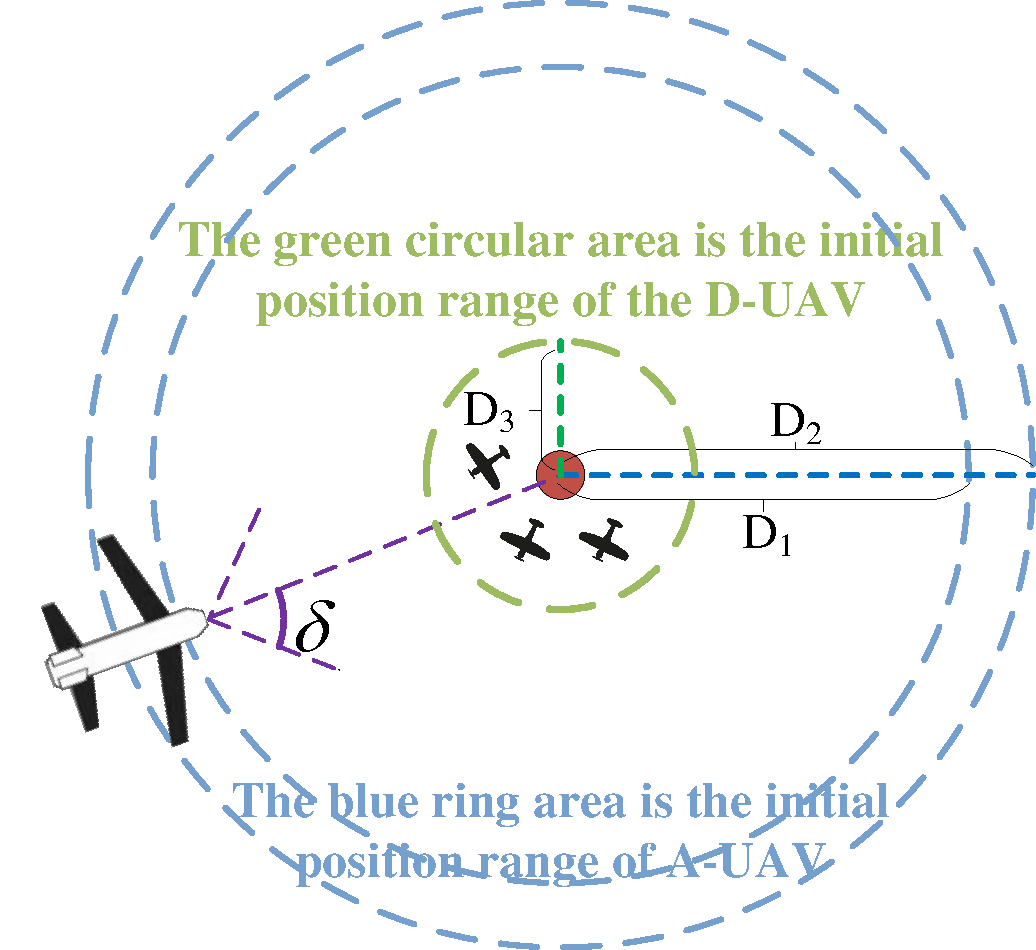
\includegraphics[width=3.0in]{chushi01.pdf}
\caption{Simulation environment configuration for training.}
\label{chushi}
\end{figure}

A representative scenario of 20 $D_{\text{UAV}}$ versus 8
$A_{\text{UAV}}$ is considered\DIFdelbegin \DIFdel{, with $D_1=100$\,m,
$D_2=1500$\,m, and $D_3=1600$\,m}\DIFdelend . Table~\ref{chushicanshu} summarizes the
\DIFdelbegin \DIFdel{UAV kinematic parameters}\DIFdelend \DIFaddbegin \DIFadd{audited three-dimensional initialization and kinematic constraints}\DIFaddend .

\begin{table*}[!t]
\centering
\caption{UAV Parameters for Attackers and Defenders}
\label{chushicanshu}
\renewcommand{\arraystretch}{1.6}
\begin{tabular}{ccccc}
\hline\hline
 & Initial \DIFdelbeginFL \DIFdelFL{position $(x,y)$ }\DIFdelendFL \DIFaddbeginFL \DIFaddFL{radius / altitude }\DIFaddendFL & Initial velocity $V$ & Initial heading $\gamma$ & Maneuverability \DIFdelbeginFL \DIFdelFL{$(n_x,n_y,V)$ }\DIFdelendFL \DIFaddbeginFL \DIFaddFL{$(n_x,n_y,n_z,V)$ }\DIFaddendFL \\ \hline
$D_{\text{UAV}}$ & \DIFdelbeginFL \DIFdelFL{$r\sim U[0,D_3]$, $\theta\sim U[0,2\pi]$ }\DIFdelendFL \DIFaddbeginFL \DIFaddFL{52.63--65.44\,m / 0\,m }\DIFaddendFL & \DIFdelbeginFL \DIFdelFL{$V_D\sim U[10,40]$}\DIFdelendFL \DIFaddbeginFL \DIFaddFL{20.32--30.02}\DIFaddendFL \,m/s & \DIFdelbeginFL \DIFdelFL{$\gamma_D\sim U[0,2\pi]$ }\DIFdelendFL \DIFaddbeginFL \DIFaddFL{$\gamma_D\in[0,2\pi]$ }\DIFaddendFL & \DIFdelbeginFL \DIFdelFL{$n_x\in[-0.1g,1g]$, $n_y\in[-1g,1g]$ }\DIFdelendFL \DIFaddbeginFL \DIFaddFL{$n_x\in[-0.1,1]$, $n_y,n_z\in[-1,1]$ }\DIFaddendFL \\
$A_{\text{UAV}}$ & \DIFdelbeginFL \DIFdelFL{$r\sim U[D_1,D_2]$, $\theta\sim U[0,2\pi]$ }\DIFdelendFL \DIFaddbeginFL \DIFaddFL{1987.72--2145.95\,m / 120\,m }\DIFaddendFL & \DIFdelbeginFL \DIFdelFL{$V_A\sim U[10,40]$}\DIFdelendFL \DIFaddbeginFL \DIFaddFL{30.23--45.87}\DIFaddendFL \,m/s & \DIFdelbeginFL \DIFdelFL{$\gamma_A\sim U[q_A-30^\circ,q_A+30^\circ]$ }\DIFdelendFL \DIFaddbeginFL \DIFaddFL{Toward defended area }\DIFaddendFL & \DIFdelbeginFL \DIFdelFL{$n_x=0$, $n_y\in[-1g,1g]$ }\DIFdelendFL \DIFaddbeginFL \DIFaddFL{Case-specific 3-D maneuver }\DIFaddendFL \\ \hline
\end{tabular}
\end{table*}

Two dynamic engagement scenarios are designed to evaluate cooperative guidance performance.
The scenario configurations are listed in Table~\ref{changjingqingkuang}.

\begin{table}[!t]
\centering
\renewcommand{\arraystretch}{1.4}
\caption{Combat Scenario Settings}
\label{changjingqingkuang}
\begin{tabular}{cccc}
\hline\hline
 & $N_{D\text{-UAV}}$ & $N_{A\text{-UAV}}$ & $A_{\text{UAV}}$ Strategy \\ \hline
Case 1 & 20 & 8 & Hybrid Evasion \\
Case 2 & 20 & 8 & Sinusoidal Maneuver \\ \hline
\end{tabular}
\end{table}




\subsection{Target Assignment Performance and Spatial Topology}
\label{subsec:assignment_results}

To evaluate the IDBO algorithm, it is benchmarked against PSO, GWO, SSA, BOA, and standard DBO. 

Fig.~\ref{fig:convergence} illustrates the statistical performance in terms of average cost convergence over iterations. IDBO significantly outperforms the baselines, reaching the lowest steady-state cost within 100~iterations. \begin{figure}[!ht] 
\centering 
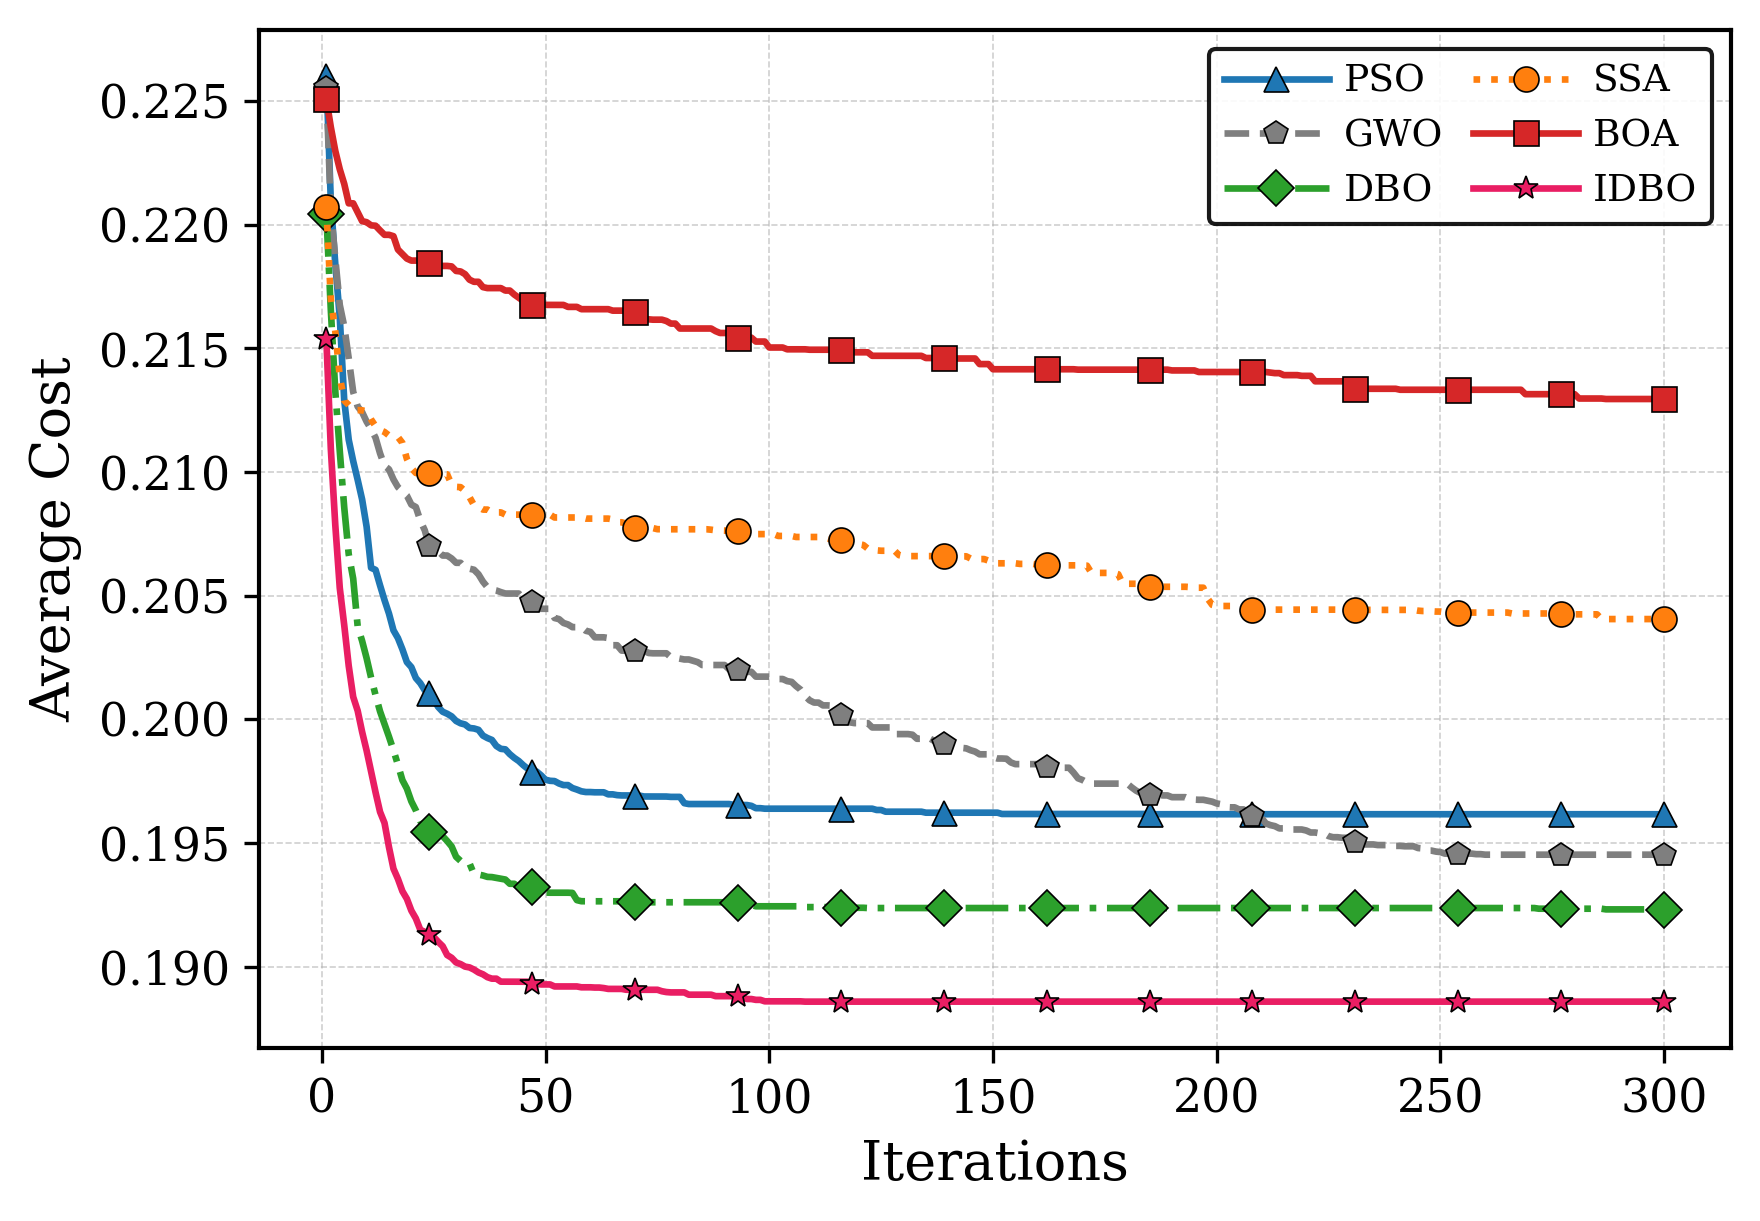
\includegraphics[width=3.25in]{convergence.png} 
\caption{Average cost convergence over iterations for target assignment algorithms.} 
\label{fig:convergence} 
\end{figure}

Furthermore, the violin plot in Fig.~\ref{fig:violin} evaluates the algorithmic robustness across multiple independent runs. It shows IDBO's compact distribution at the lowest median cost, highlighting its superior stability and consistency compared to the other heuristic methods.

\begin{figure}[!ht] 
\centering 
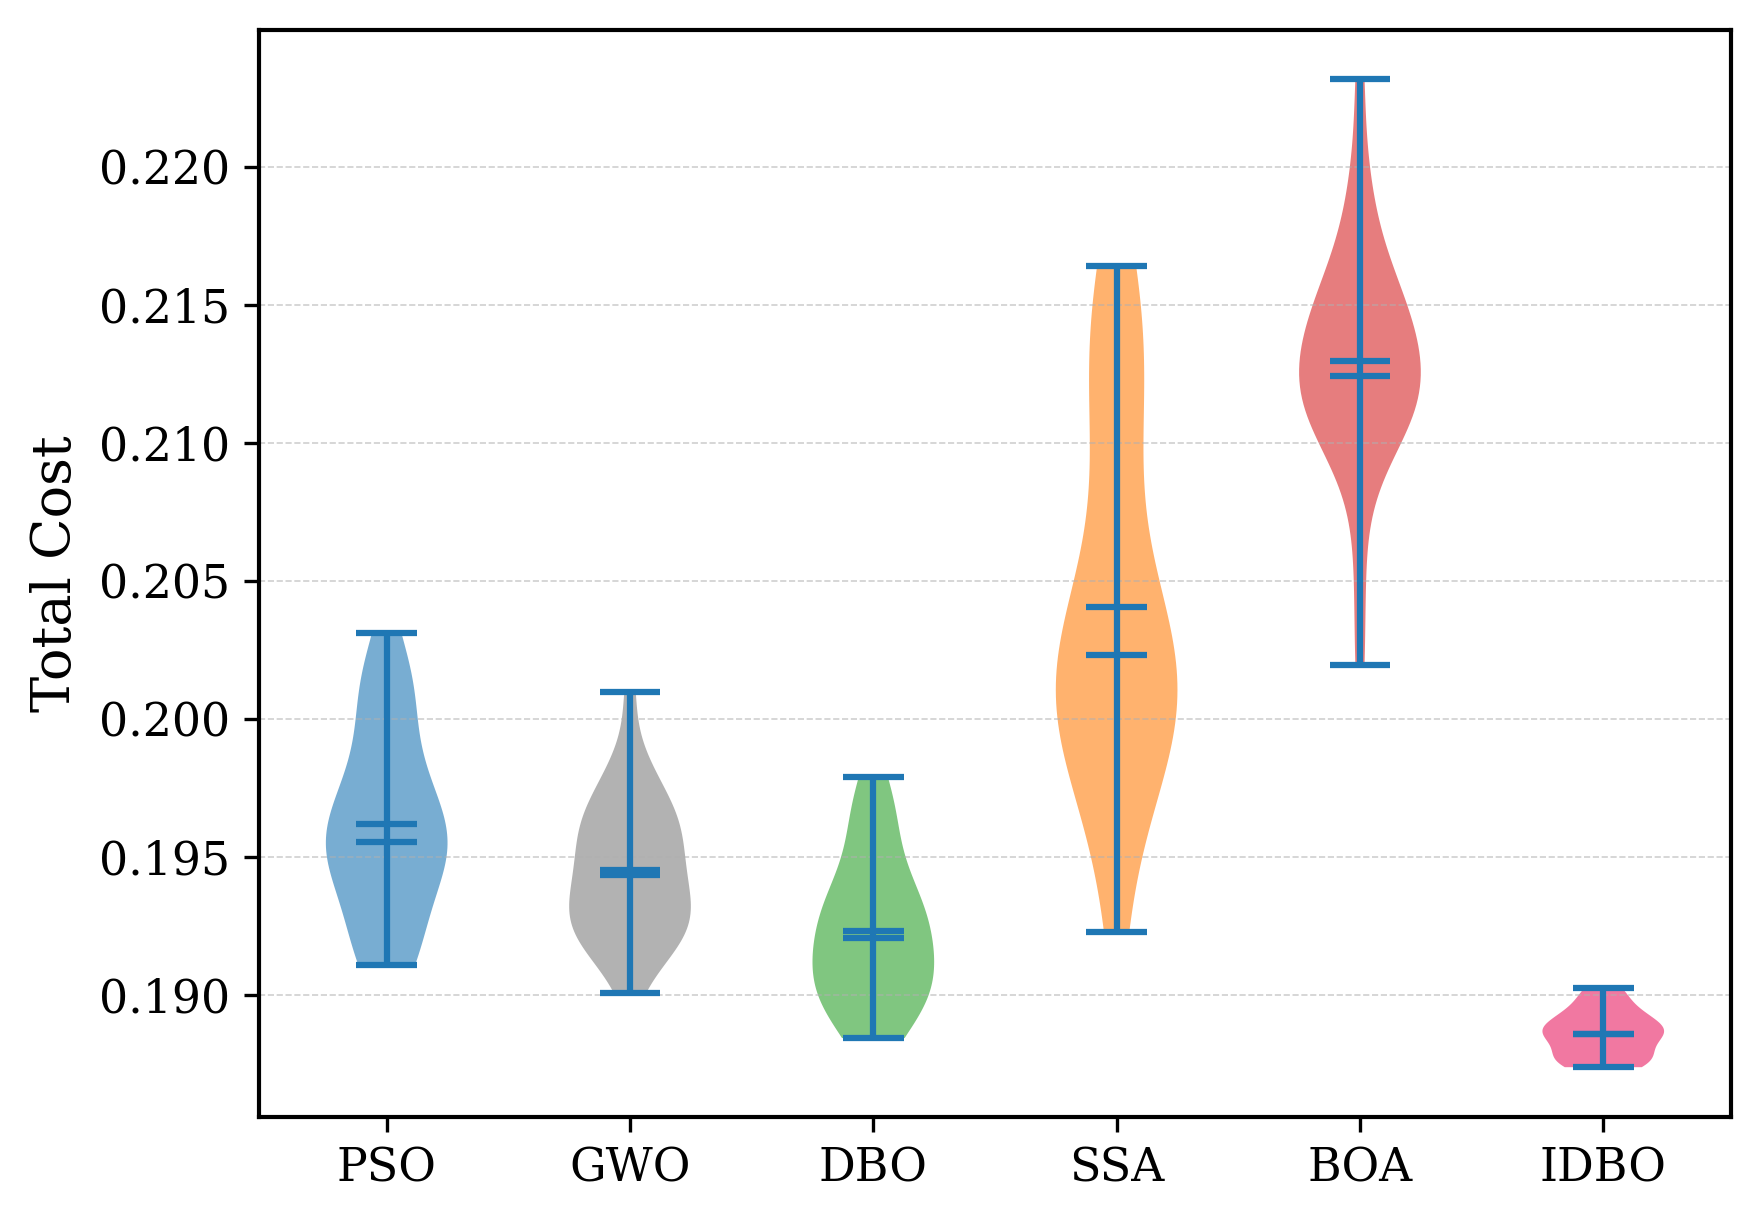
\includegraphics[width=3.2in]{violin.png} 
\caption{Violin plot of total cost distribution evaluating algorithm robustness.} 
\label{fig:violin} 
\end{figure}

\DIFaddbegin \DIFadd{To isolate the effect of the IDBO coefficient schedule, we additionally
performed a 30-paired-seed capacity-constrained study with population 40 and
100 iterations. Fig.~\ref{fig:idbo_schedule_delay}(a) compares the decaying
mutation strength \(0.36\to0.04\) with a fixed value of 0.18. The final costs
are \(0.006975\pm0.000141\) and \(0.006942\pm0.000083\), respectively; the
median iterations required to enter each run's final 1\% band are 19.0 and
21.5. The decaying schedule therefore reaches its own terminal band slightly
earlier, but it does not improve the final objective in this audit.
}

\DIFadd{Fig.~\ref{fig:idbo_schedule_delay}(b) evaluates the communication primitive
used by consensus bidding on a 20-node graph with 1\% packet dropout. Mean
dissemination rounds are 4.00, 5.80, 7.07, and 9.17 for maximum link delays of
0, 1, 2, and 4 rounds. Removing one node still allows the connected 19-node
subgraph to disseminate all remaining timestamped source records in
\(7.17\pm0.46\) rounds. These results quantify the expected delay-dependent
communication cost; they are not substituted for the optimizer convergence
curves in Figs.~\ref{fig:convergence} and \ref{fig:violin}.
}

\DIFadd{We also vary the probability-model weights over
\(w_{\mathrm{ZEM}}\in\{0.3,0.5,0.7\}\), with
\(w_\sigma=1-w_{\mathrm{ZEM}}\). The corresponding optimized objective means
are 0.004611, 0.006986, and 0.009956. Because changing these weights changes
the numerical objective itself, the absolute values are interpreted as the
expected tradeoff between predicted miss tendency and angular advantage,
rather than ranked as measurements on one invariant scale.
}

\begin{figure}[!t]
\centering
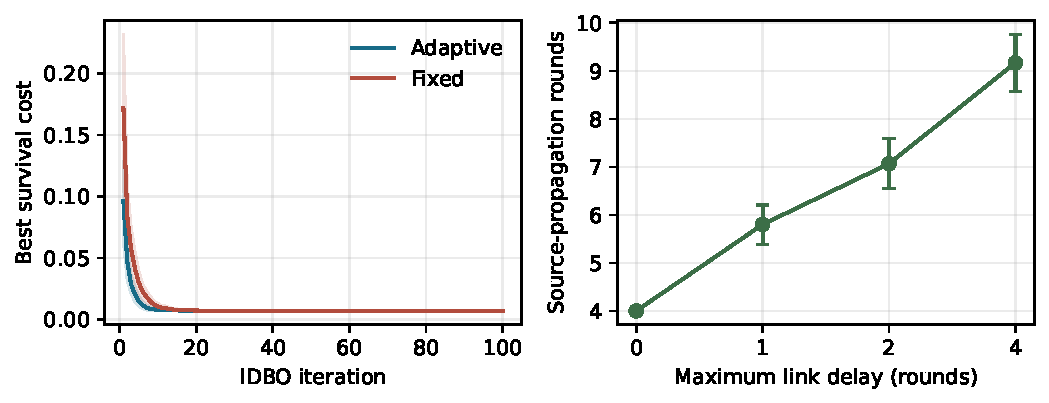
\includegraphics[width=3.45in]{idbo_ablation_delay.pdf}
\caption{\DIFaddFL{Additional IDBO audit. (a) Paired-seed coefficient-schedule
comparison. (b) Timestamped information-dissemination rounds under bounded
delay and 1\% packet dropout.}}
\label{fig:idbo_schedule_delay}
\end{figure}

\DIFaddend The optimal assignment mapping generated by the algorithm is visualized in Fig.~\ref{fig:assignment_topology}. Attackers $A_1$--$A_4$ are each allocated three defenders, while $A_5$--$A_8$ are intercepted by two defenders each, perfectly respecting the per-target capacity constraint $L_{\max}$ and ensuring sufficient numerical superiority for cooperative strikes.

\DIFaddbegin \DIFadd{The one-based target vector exported after consensus is
}\[
[1,2,3,4,5,6,7,8,\;1,2,3,4,5,6,7,8,\;1,2,3,4].
\]
\DIFadd{The same vector is stored in the three-dimensional case preset and consumed by
ART-MAPPO without remapping, providing a direct assignment-to-guidance
interface between the two stages.
}

\DIFaddend \begin{figure}[!ht]
\centering
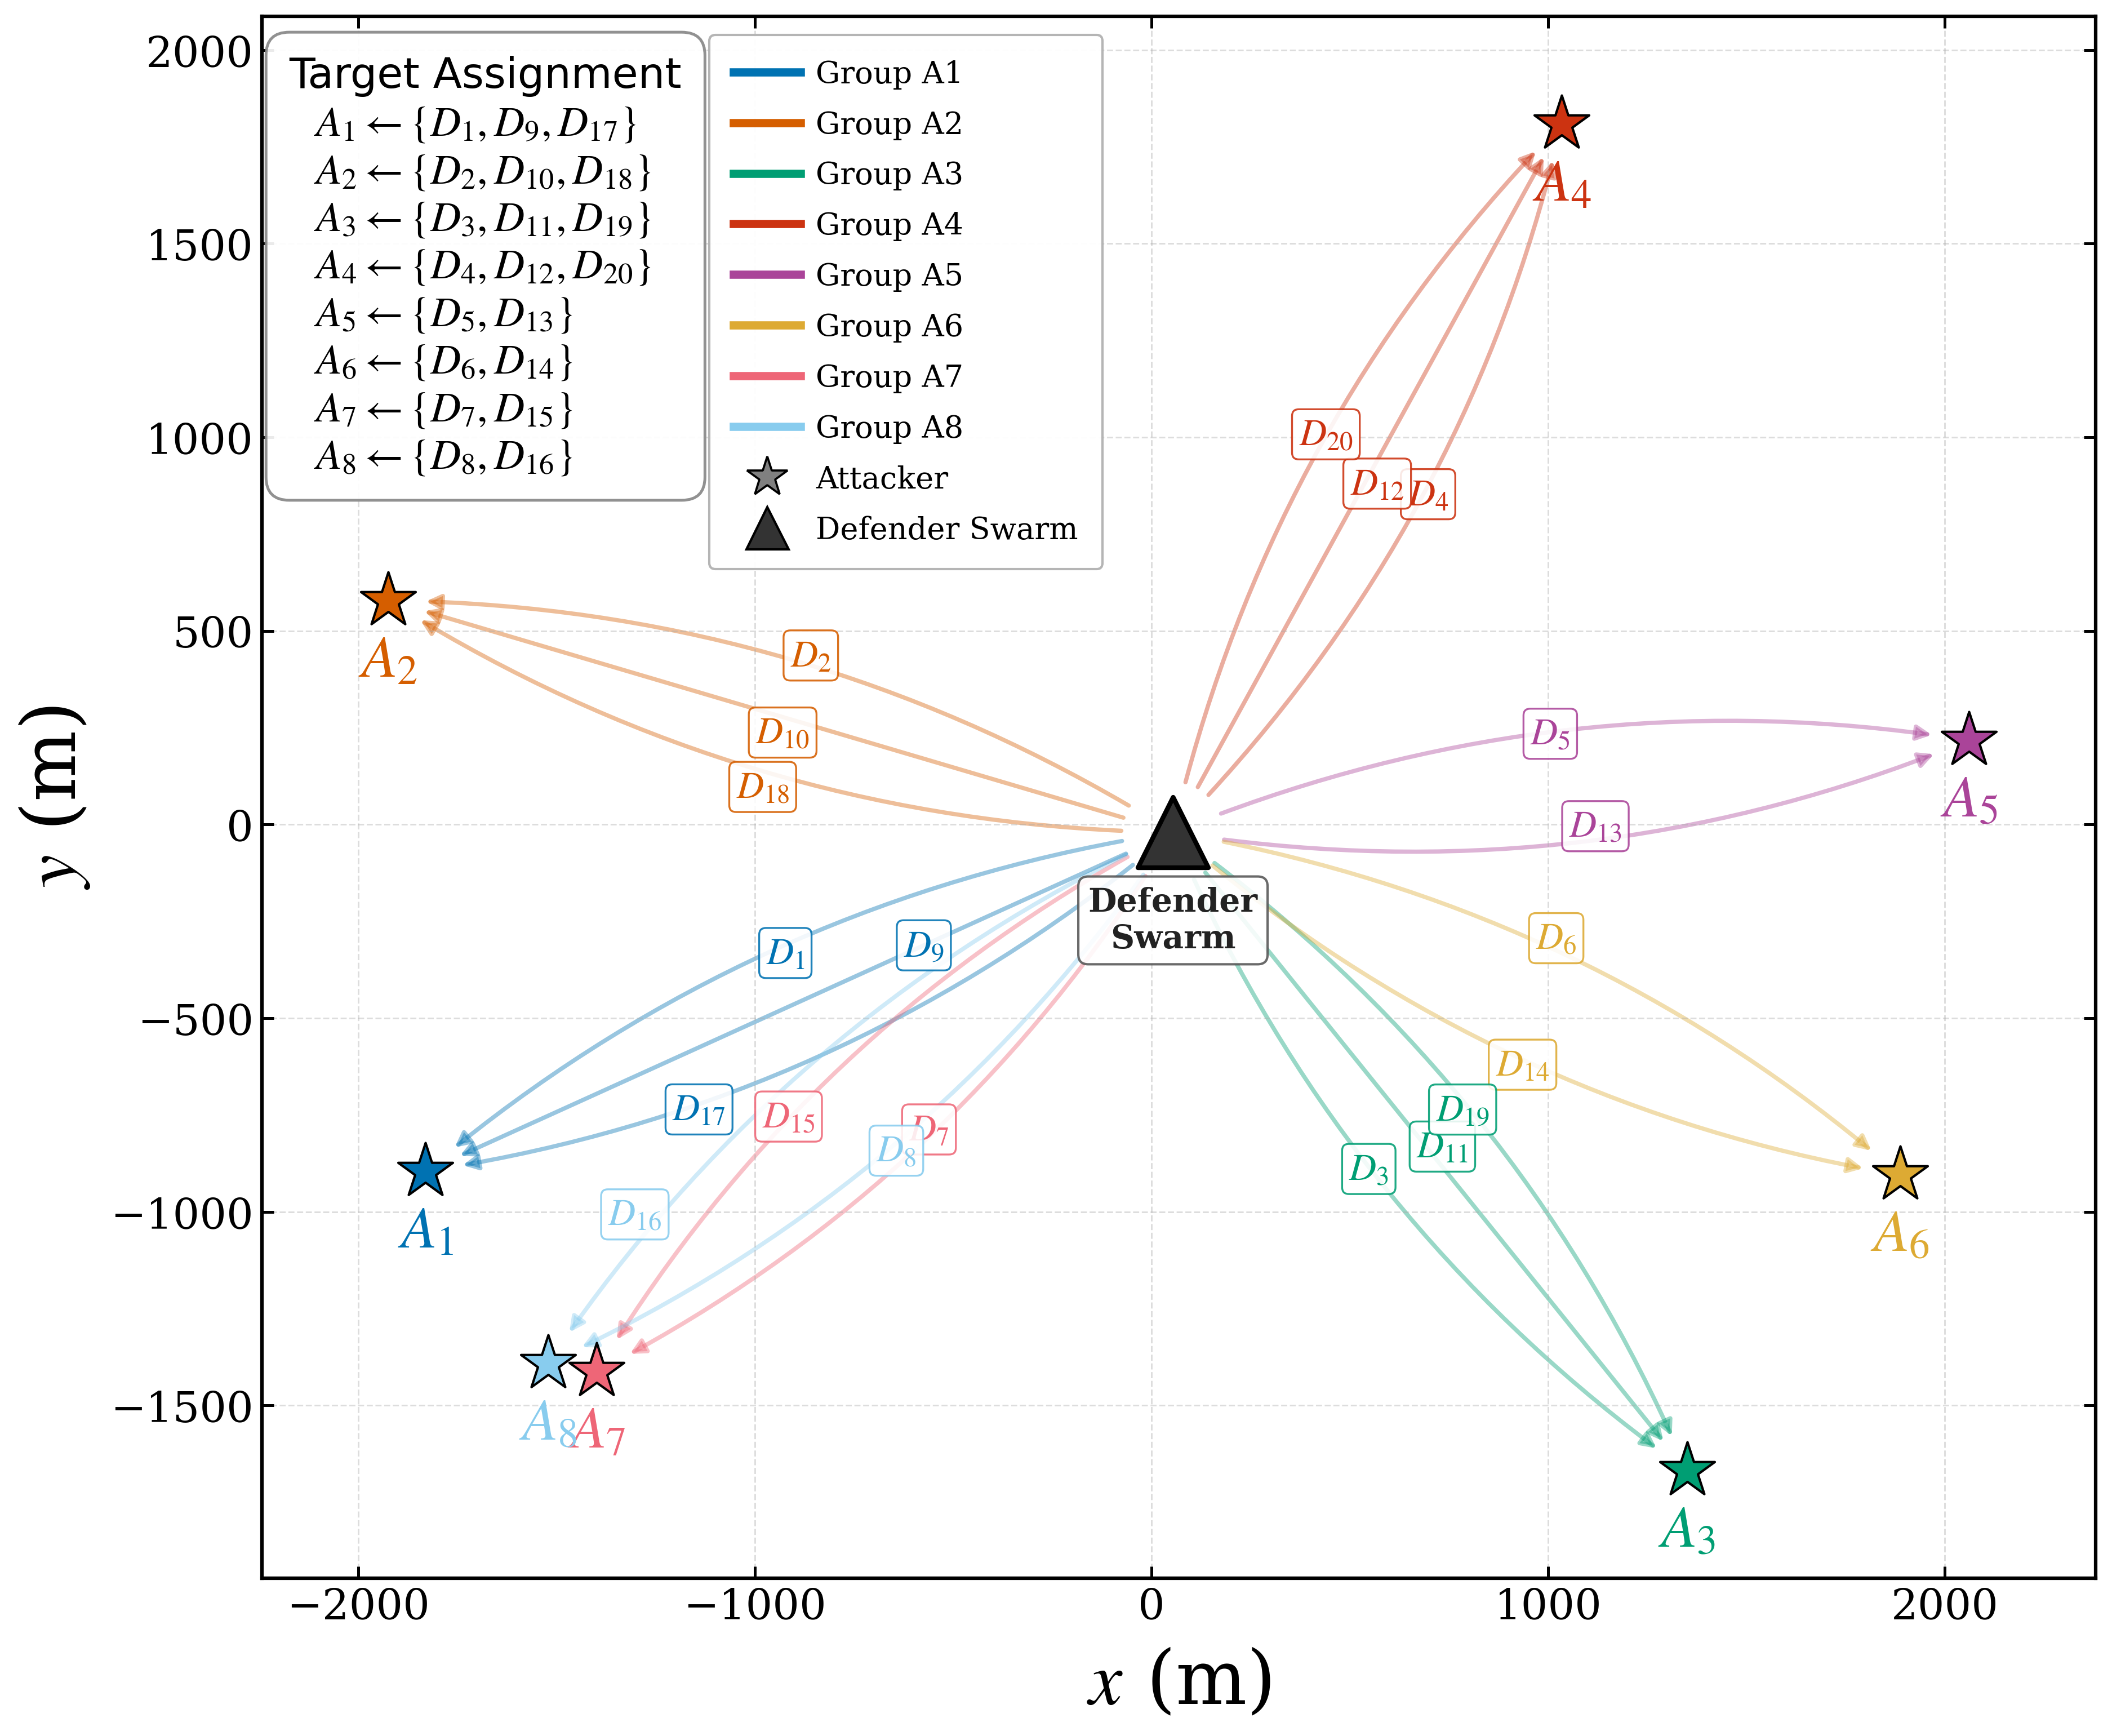
\includegraphics[width=3.2in]{target_assignment_topology.png}
\caption{Visualized spatial topology of the target assignment results.}
\label{fig:assignment_topology}
\end{figure}








\subsection{RL Model Training and Convergence Analysis}
\label{subsec:training}

To evaluate the learning efficiency and robustness of the proposed ART-MAPPO,
comparative training experiments were conducted against standard MAPPO, IPPO,
IA2C, and IQL. All models were trained over 10,000 episodes with a maximum
horizon of \DIFdelbegin \DIFdel{25 }\DIFdelend \DIFaddbegin \DIFadd{1500 simulation }\DIFaddend steps per episode. To ensure statistical
significance and eliminate the bias of favorable network initialization, all
learning curves in Fig.~\ref{fig:training_convergence} are averaged across 5
independent random seeds, with the shaded regions denoting the standard
deviation.

As illustrated in Fig.~\ref{fig:training_convergence}(a), ART-MAPPO demonstrates a superior learning paradigm, achieving the highest asymptotic normalized reward of $8.97 \pm 0.64$ (averaged over the final 500 episodes). This represents a notable performance improvement of 8.2\%, 12.3\%, 14.4\%, and 29.8\% over IQL, MAPPO, IPPO, and IA2C, respectively. The advantage of ART-MAPPO is particularly pronounced during the intermediate training phase. By episode 4,000, ART-MAPPO establishes a significant performance leap, outperforming standard MAPPO by 43.6\% and IQL by 16.6\%, highlighting its ability to rapidly escape local optima early in the training process.

Furthermore, the proposed method exhibits accelerated convergence alongside enhanced training stability. When evaluated on a 100-episode smoothed curve, ART-MAPPO reaches 90\% of its optimal asymptotic performance by episode 5,591. In contrast, the most competitive baseline, IQL, requires 6,477 episodes (a 13.7\% delay), while standard MAPPO lags significantly, requiring 7,654 episodes. Regarding algorithmic stability, ART-MAPPO maintains a tight variance across random seeds ($\sigma = 0.64$), whereas standard MAPPO exhibits a standard deviation of 1.34 (approximately twice as large). This confirms that the proposed enhancements effectively mitigate the high-variance gradient updates typical in multi-agent policy-based methods.

These macroscopic performance gains are directly supported by the network-level metrics. The critic loss (Fig.~\ref{fig:training_convergence}(b)) of ART-MAPPO converges to the lowest steady-state error with minimal oscillation, a direct consequence of the dual-clip mechanism and adaptive KL penalty. Concurrently, the policy entropy (Fig.~\ref{fig:training_convergence}(c)) demonstrates an optimal, gradual decay trajectory, validating that the trust-modulated exploration mechanism successfully balances early-stage extensive state-space exploration with late-stage strict policy exploitation.

It should be emphasized that the convergence discussed here is empirical training
convergence rather than a global optimality guarantee for the nonconvex MARL problem. In
particular, ART-MAPPO inherits the practical convergence interpretation of PPO-style policy
gradient methods: a stable learning process is indicated by a saturating reward curve, bounded
inter-seed variance, a nondivergent critic loss, and a gradually decreasing policy entropy.
The dual-clip objective and adaptive KL penalty do not prove convergence to the global
optimum; instead, they restrict the policy update magnitude and reduce destructive policy
oscillations caused by large importance-sampling ratios. Therefore, the convergence claim for
ART-MAPPO should be understood as statistically validated stability and asymptotic performance
under the tested training settings, supported by the five-seed learning curves and the
network-level diagnostics in Fig.~\ref{fig:training_convergence}.

\begin{figure}[!t]
\centering
\subfloat[Training Reward]{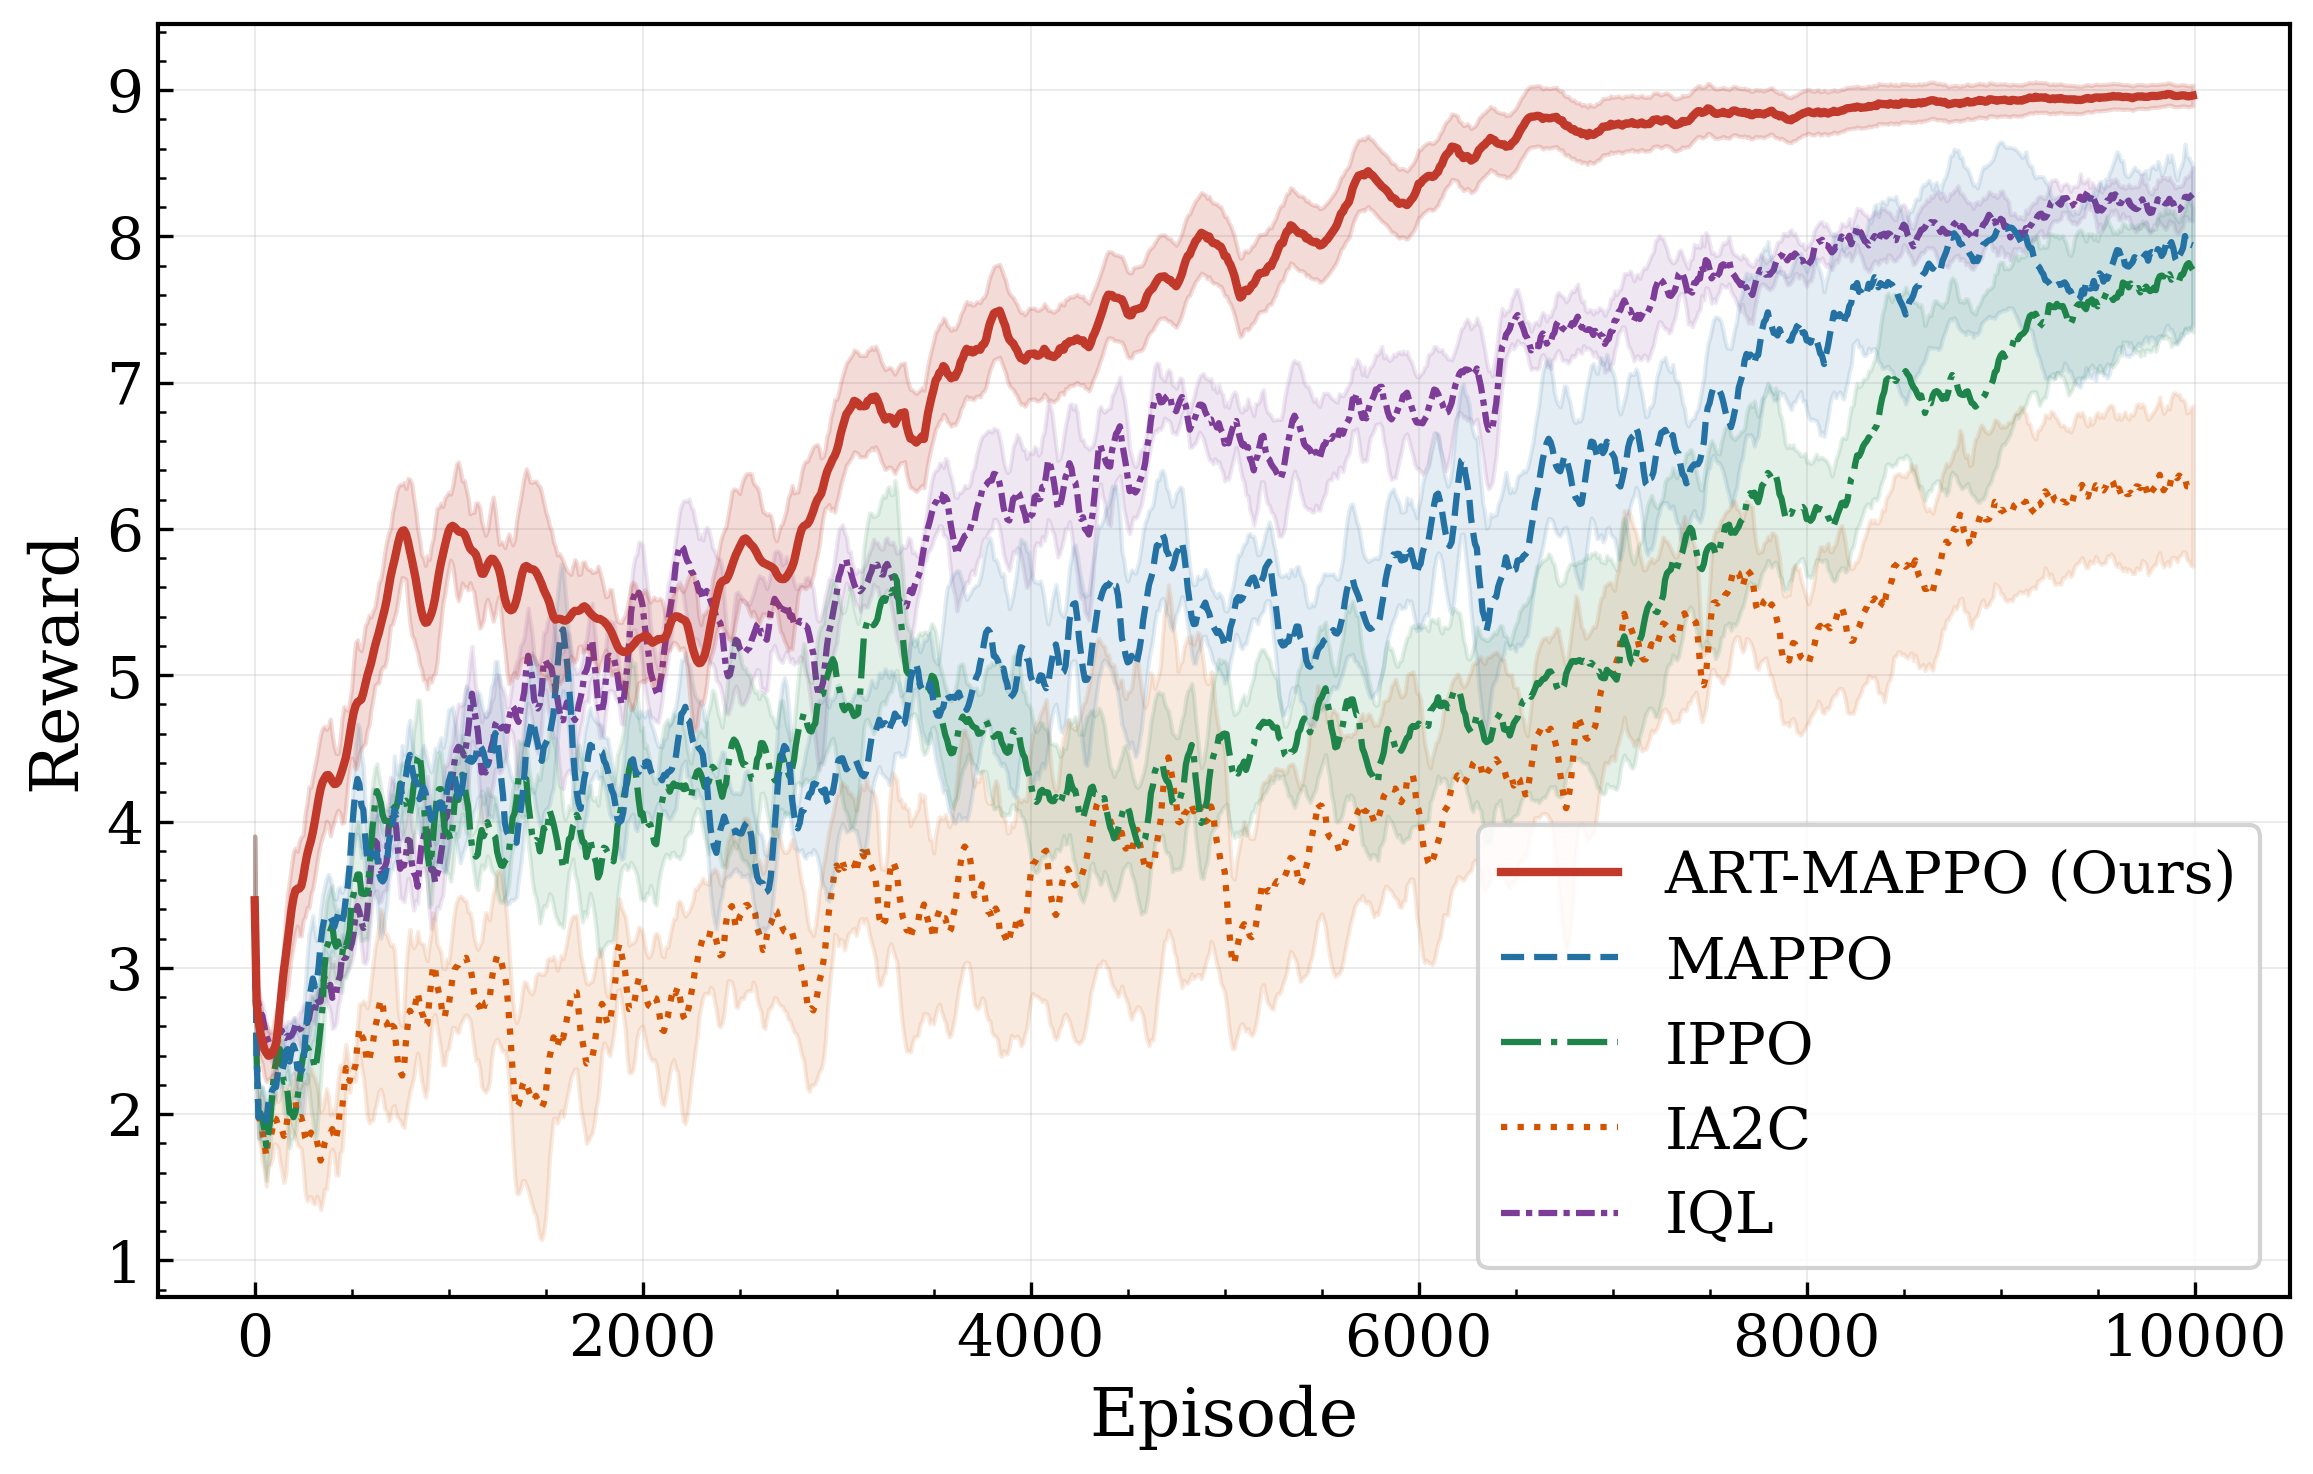
\includegraphics[width=3.0in]{fig_a_reward.png}}
\hfill
\subfloat[Critic Loss]{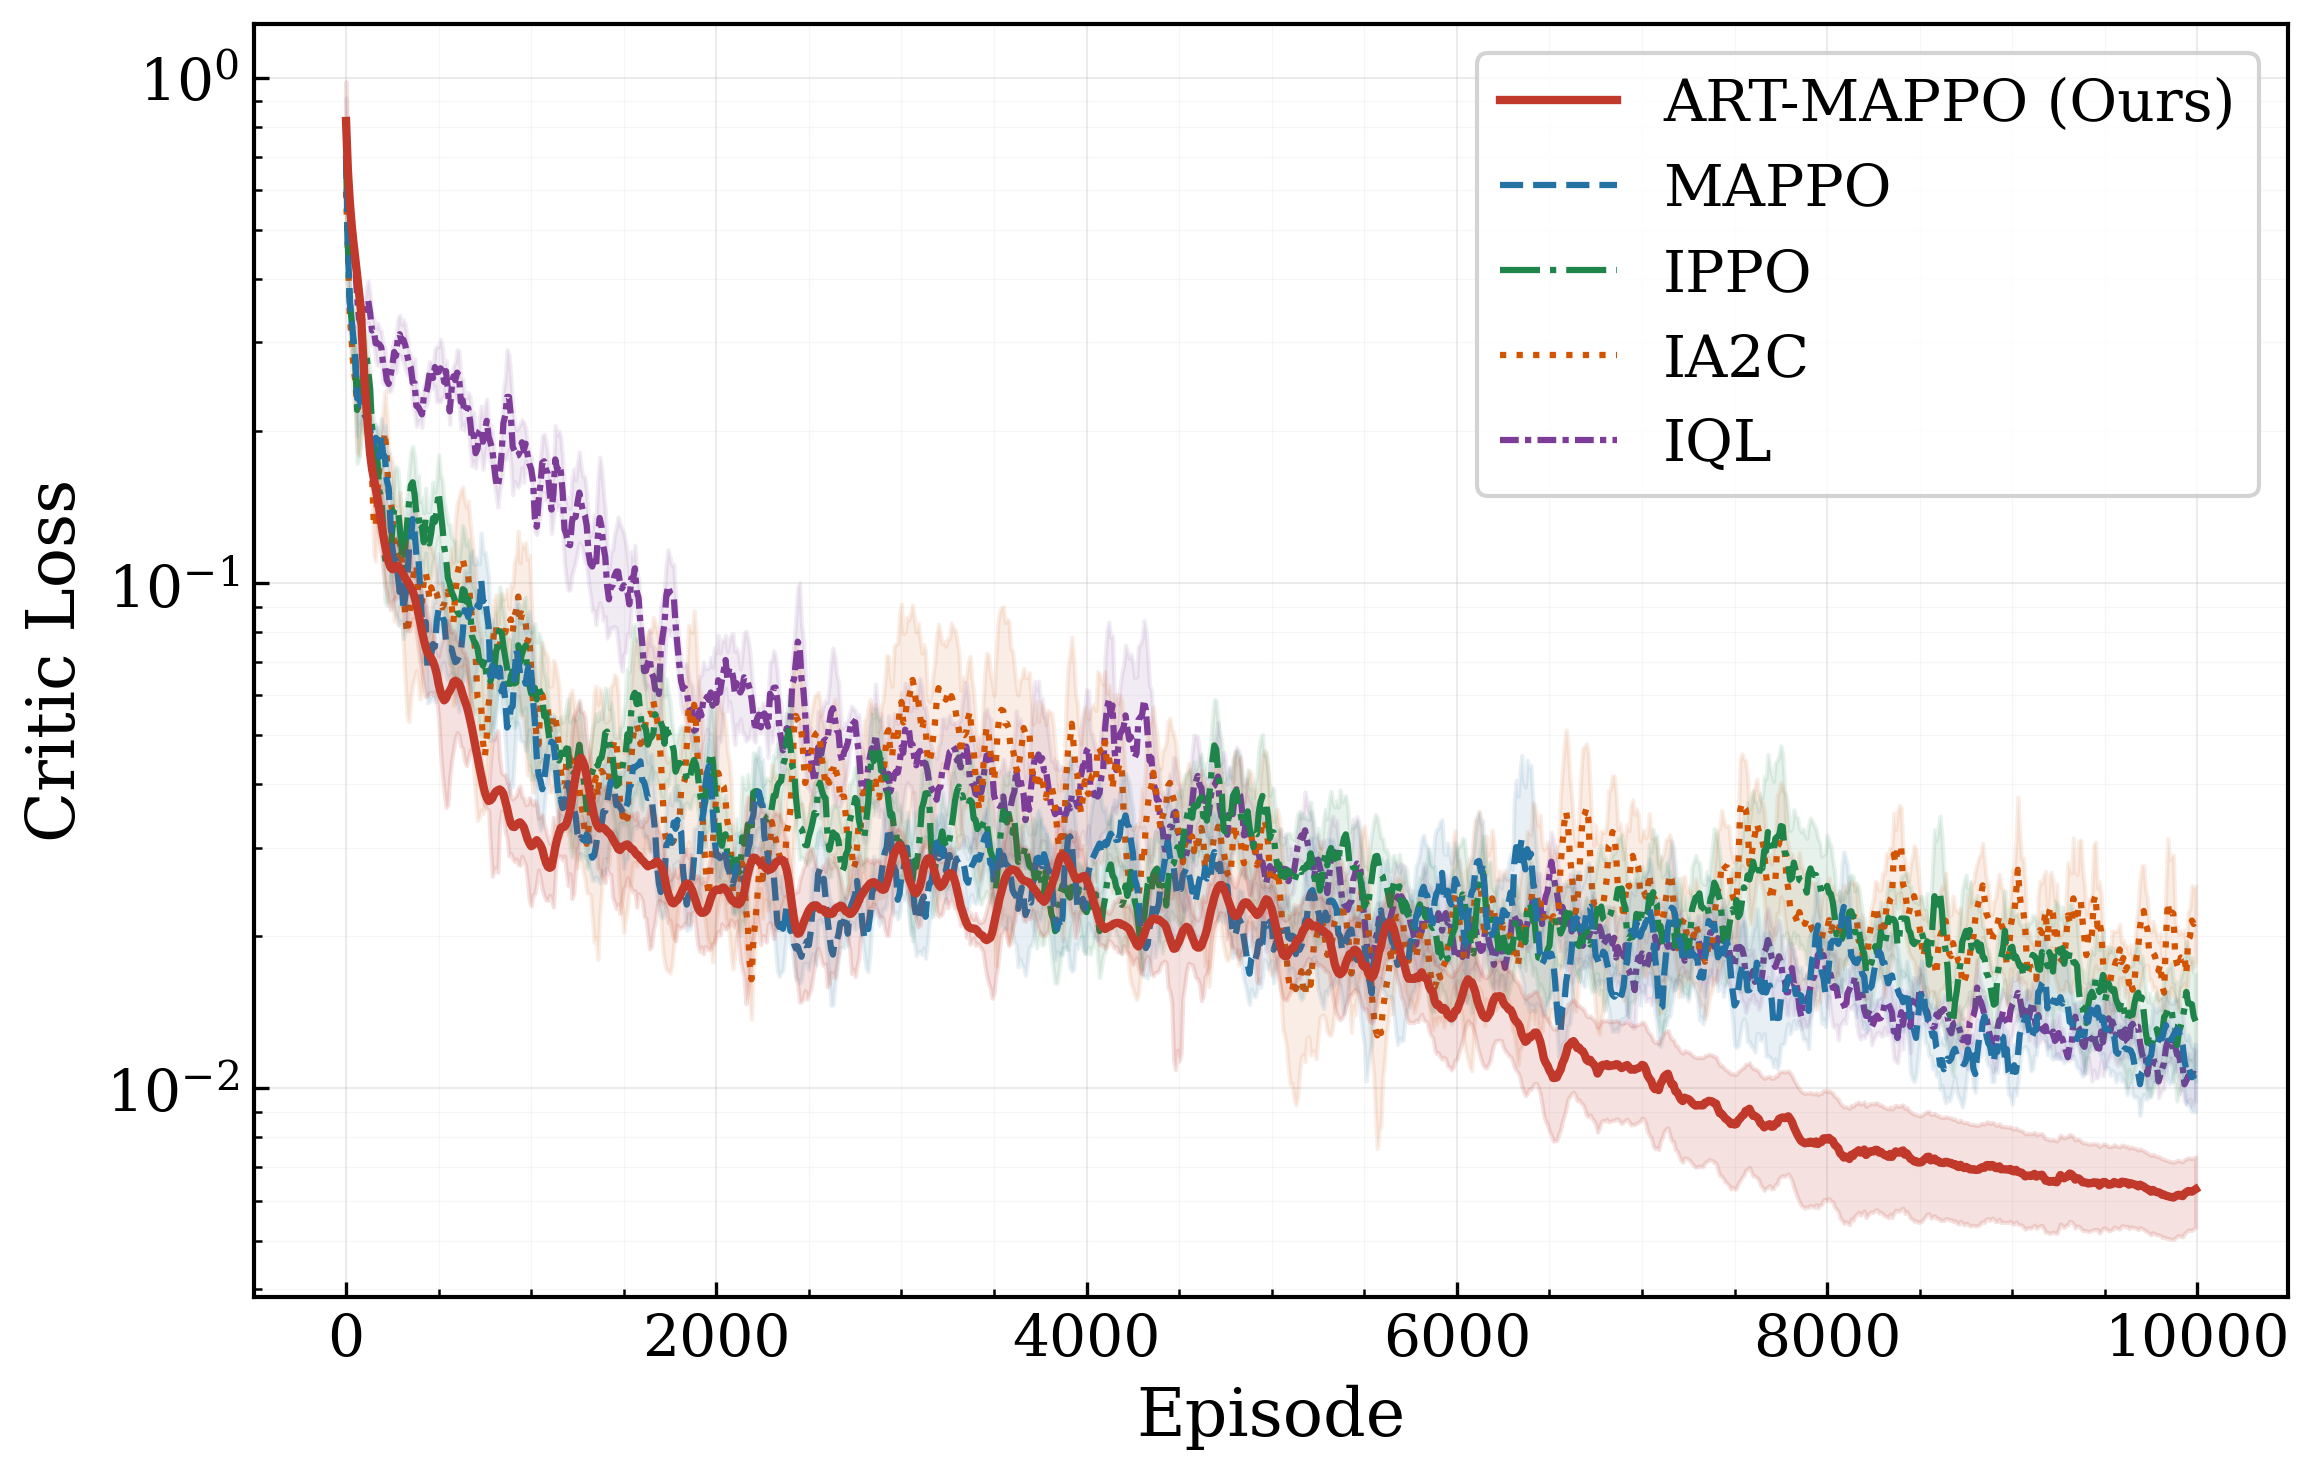
\includegraphics[width=3.0in]{fig_b_critic_loss.png}}
\hfill
\subfloat[Policy Entropy]{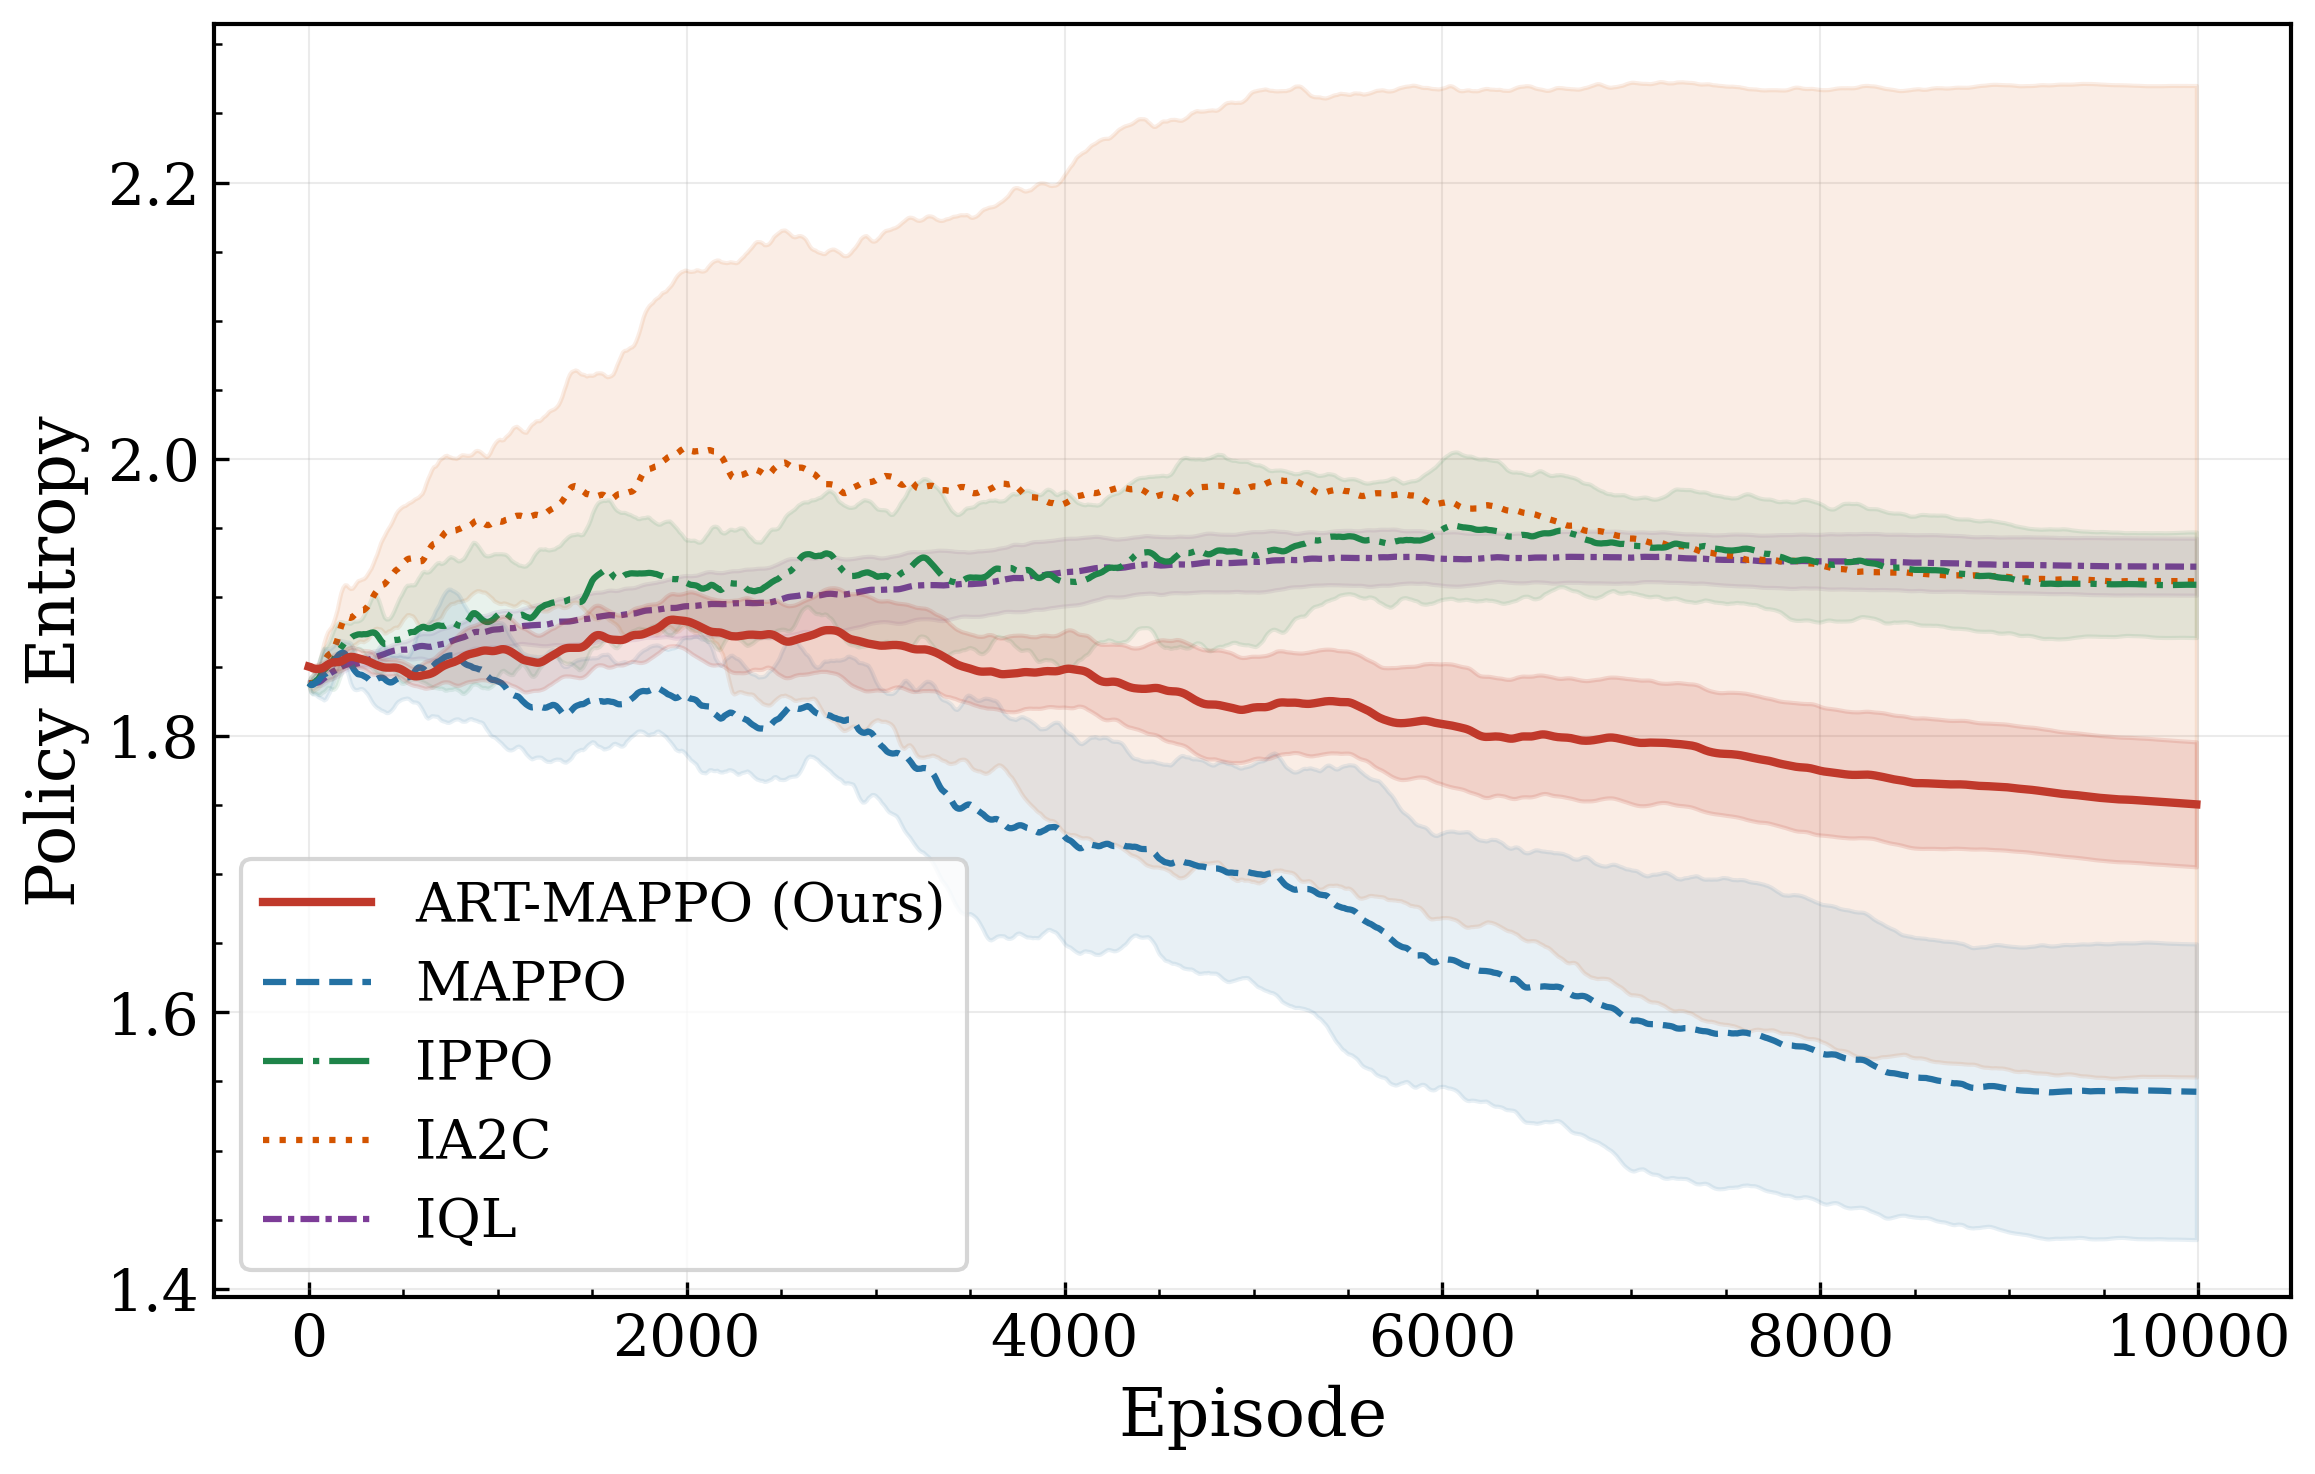
\includegraphics[width=3.0in]{fig_c_entropy.png}}
\caption{Comparative training curves of ART-MAPPO and baseline algorithms over 10,000 episodes. Solid lines and shaded regions represent the mean and standard deviation across 5 independent random seeds, respectively. Notably, ART-MAPPO achieves the highest asymptotic reward (+12.3\% over standard MAPPO) and the fastest convergence rate (reaching 90\% optimality by episode 5,591), while demonstrating significantly enhanced training stability.}
\label{fig:training_convergence}
\end{figure}


%%%%-------------------------------------------------------------------------------------------

\subsection{Cooperative Interception against Maneuvering Targets}
\label{subsec:cases}

Based on the optimal assignment topology, we evaluate the terminal cooperative guidance
performance against two maneuvering scenarios, each benchmarked against \DIFdelbegin \DIFdel{classical PN }\DIFdelend \DIFaddbegin \DIFadd{a
capacity-matched PN implementation. For each method--case combination, the
V10 results are organized into three complementary composites: engagement
geometry and range, three-dimensional motion and control, and temporal
coordination. The motion-and-control panels are ordered as \(n_x\), \(n_y\),
\(n_z\), \(V_D\), yaw \(\psi_D\), and pitch \(\theta_D\). The yaw angle is
temporally unwrapped across the \(\pm\pi\) branch cut. Pitch is reconstructed
from the recorded three-dimensional trajectory as
\(\theta_D=\operatorname{atan2}(v_z,\sqrt{v_x^2+v_y^2})\). The legacy
\texttt{heading} export contains the same horizontal-plane angle as \(\psi_D\)
and is therefore not duplicated. The D-UAV color legend in
Fig.~\ref{fig:case1_mappo_kine} is shared by all four motion-and-control
composites}\DIFaddend .

\subsubsection{Case~1: Interception against Evasive Maneuvering Targets}

In this scenario, the attacking UAVs (\DIFdelbegin \DIFdel{$A_{\text{UAV}}$}\DIFdelend \DIFaddbegin \DIFadd{\(A_{\text{UAV}}\)}\DIFaddend ) initially execute a
constant-\DIFdelbegin \DIFdel{$g$ }\DIFdelend \DIFaddbegin \DIFadd{\(g\) }\DIFaddend evasive maneuver and transition to \DIFdelbegin \DIFdel{proportional navigation (PN ) }\DIFdelend \DIFaddbegin \DIFadd{PN }\DIFaddend guidance after 15\,s.
\DIFdelbegin \DIFdel{The defending swarm is tasked with neutralizing these highly dynamic threats utilizing the pre-computed assignment topology.
}%DIFDELCMD < 

%DIFDELCMD < %%%
\DIFdelend Fig.~\ref{fig:case1_mappo_traj} \DIFdelbegin \DIFdel{illustrates the 2D engagement trajectories generated by the proposed }\DIFdelend \DIFaddbegin \DIFadd{shows that }\DIFaddend ART-MAPPO \DIFdelbegin \DIFdel{algorithm. Guided by the intelligent policy, the defending swarm effectively divides into eight coordinated combat units.
Despite the evasive maneuvers of the targets,
}\DIFdelend \DIFaddbegin \DIFadd{divides the 20 defenders
into the eight assigned groups and closes every three-dimensional engagement.
The horizontal view distinguishes the group-dependent approach directions,
the 3-D view confirms the required climb from zero initial defender altitude,
and the range histories decrease to the 3-m hit threshold. The first and last
}\DIFaddend ART-MAPPO \DIFdelbegin \DIFdel{generates remarkably smooth and direct pursuit curves, enabling all interceptors to successfully converge on their respective targets without unnecessary detours}\DIFdelend \DIFaddbegin \DIFadd{impacts occur at 24.45 and 30.35\,s, respectively}\DIFaddend .

\DIFdelbegin %DIFDELCMD < \begin{figure}[!ht]
%DIFDELCMD < %%%
\DIFdelendFL \DIFaddbeginFL \begin{figure*}[!t]
\DIFaddendFL \centering
\DIFdelbeginFL %DIFDELCMD < 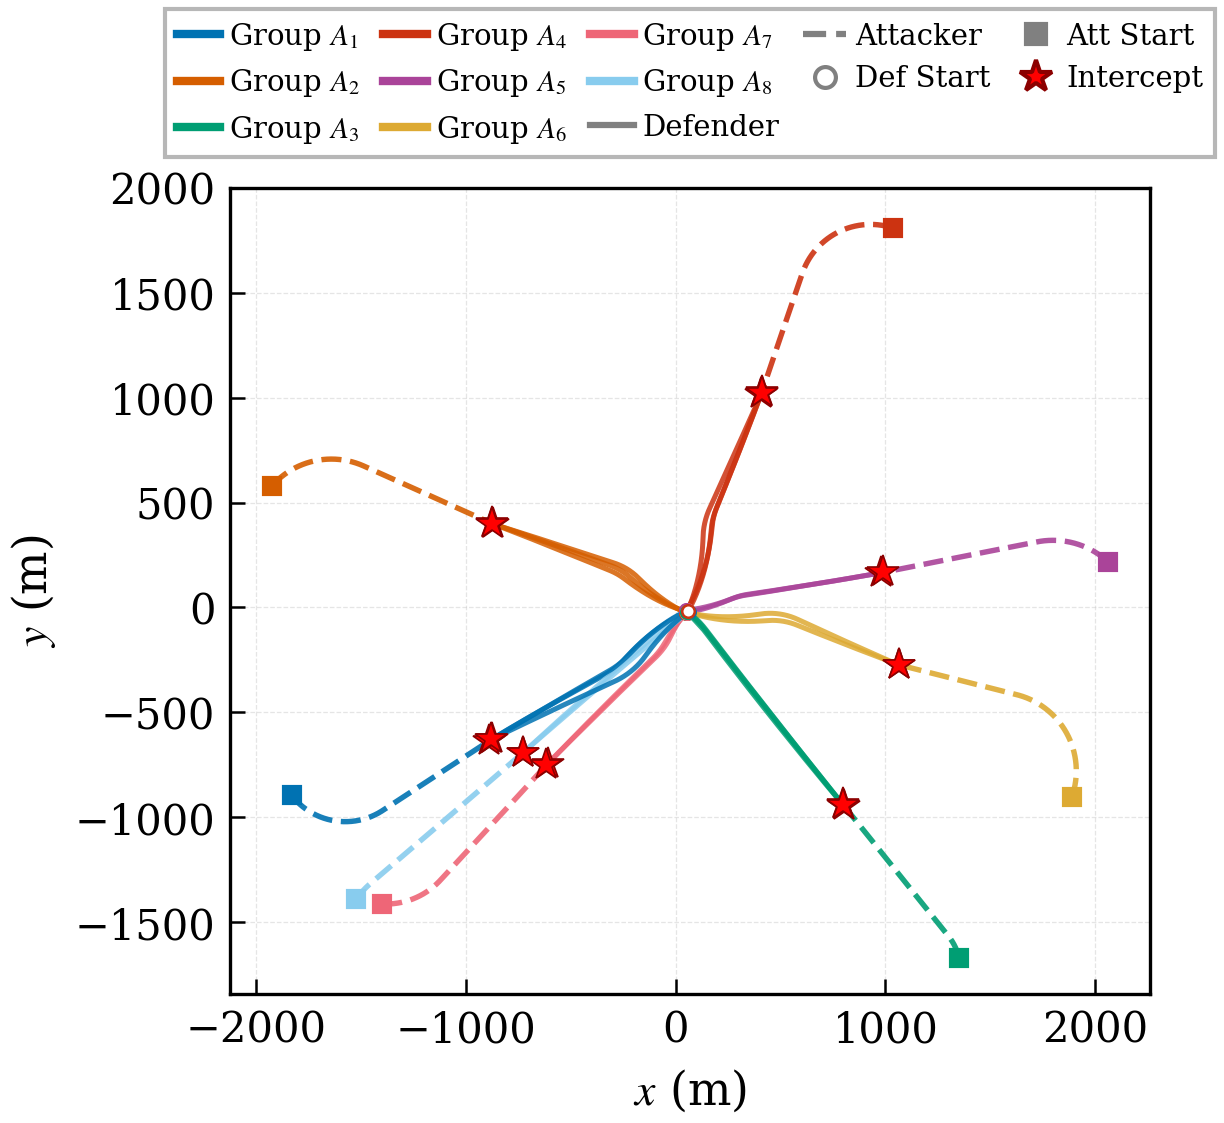
\includegraphics[width=3.2in]{mappo_nopn_trajectory.png}
%DIFDELCMD < %%%
\DIFdelendFL \DIFaddbeginFL \subfloat[Horizontal trajectory]{
\includegraphics[width=2.25in]{new_sim_fig/figures_v10/mappo/mappo_nopn_trajectory.png}}\hfill
\subfloat[Three-dimensional trajectory]{
\includegraphics[width=2.25in]{new_sim_fig/figures_v10/mappo/mappo_nopn_trajectory_3d.png}}\hfill
\subfloat[Interceptor--target range]{
\includegraphics[width=2.25in]{new_sim_fig/figures_v10/mappo/mappo_nopn_distance.png}}
\DIFaddendFL \caption{\DIFdelbeginFL \DIFdelFL{Engagement trajectories of the defending swarm using }\DIFdelendFL ART-MAPPO \DIFdelbeginFL \DIFdelFL{in }\DIFdelendFL \DIFaddbeginFL \DIFaddFL{engagement geometry and range histories for }\DIFaddendFL Case~1. \DIFaddbeginFL \DIFaddFL{The
horizontal and three-dimensional paths show the assigned approach geometry,
while the range panel verifies monotonic terminal closure to the hit region.}\DIFaddendFL }
\label{fig:case1_mappo_traj}
\DIFdelbeginFL %DIFDELCMD < \end{figure}
%DIFDELCMD < %%%
\DIFdelend \DIFaddbegin \end{figure*}
\DIFaddend 

\DIFdelbegin \DIFdel{To deeply analyze the operational efficiency and constraint adherence of the proposed method, Fig.~\ref{fig:case1_mappo_kine} presents the comprehensive kinematic and control profiles of ART-MAPPO. Most critically, the normal acceleration ($n_y$) profile }\DIFdelend \DIFaddbegin \DIFadd{The six panels }\DIFaddend in Fig.~\ref{fig:case1_mappo_kine} \DIFdelbegin \DIFdel{(a) highlights the safety and robustness of the learned policy: ART-MAPPO strictly bounds its lateral overload within the physical $\pm1$\,g limit throughout the entire mid-course and terminal phases, completely avoiding the risk of actuator saturation. Furthermore, the heading angles smoothly adjust to the optimal collision course (}\DIFdelend \DIFaddbegin \DIFadd{expose the mechanism behind
this closure. Positive \(n_x\) accelerates the defenders toward the 40-m/s
speed ceiling, while \(n_y\) steers the horizontal collision courses and
\(n_z\) produces the climb visible in }\DIFaddend Fig.~\DIFdelbegin \DIFdel{\ref{fig:case1_mappo_kine}}\DIFdelend \DIFaddbegin \DIFadd{\ref{fig:case1_mappo_traj}}\DIFaddend (b)\DIFdelbegin \DIFdel{).
As shown in the velocity ($V_D$) and axial acceleration ($n_x$) profiles (Fig.~\ref{fig:case1_mappo_kine}(c) and (d)), ART-MAPPO actively manages its forward energy, commanding maximum axial acceleration early in the engagement to rapidly reach the speed limit of 40}\DIFdelend \DIFaddbegin \DIFadd{.
The yaw histories separate according to target bearing without branch-cut
jumps. The pitch angles remain small because the required 53--69-m terminal
altitudes are accumulated over roughly one kilometre of horizontal travel;
their plotted magnitude remains below approximately 0.12}\DIFaddend \,\DIFdelbegin \DIFdel{m/s. This intelligent energy management dramatically minimizes the overall interception duration}\DIFdelend \DIFaddbegin \DIFadd{rad. The raw
three-axis maxima are \([0.9882,0.9975,0.6061]\), inside the prescribed action
envelope}\DIFaddend .

\DIFdelbegin %DIFDELCMD < \begin{figure}[!ht]
%DIFDELCMD < %%%
\DIFdelendFL \DIFaddbeginFL \begin{figure*}[!t]
\DIFaddendFL \centering
\DIFdelbeginFL %DIFDELCMD < 
\includegraphics[width=3.0in]{standalone_duav_legend.png}
%DIFDELCMD < \subfloat[Normal acceleration $n_y$]{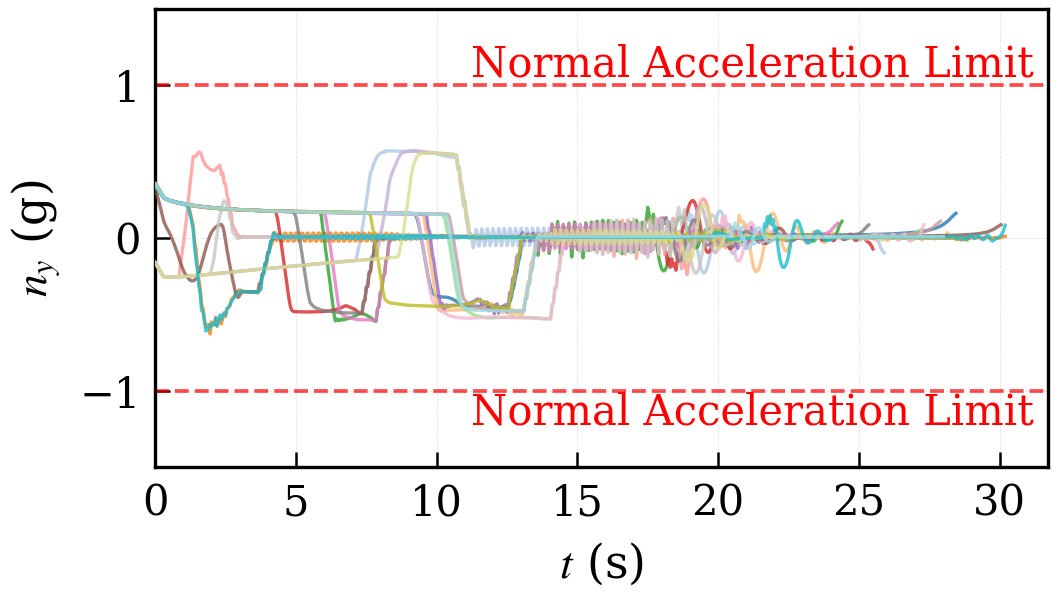
\includegraphics[width=3.0in]{mappo_nopn_ny.png}}
%DIFDELCMD < \hfil
%DIFDELCMD < \subfloat[Heading angle $\gamma_D$]{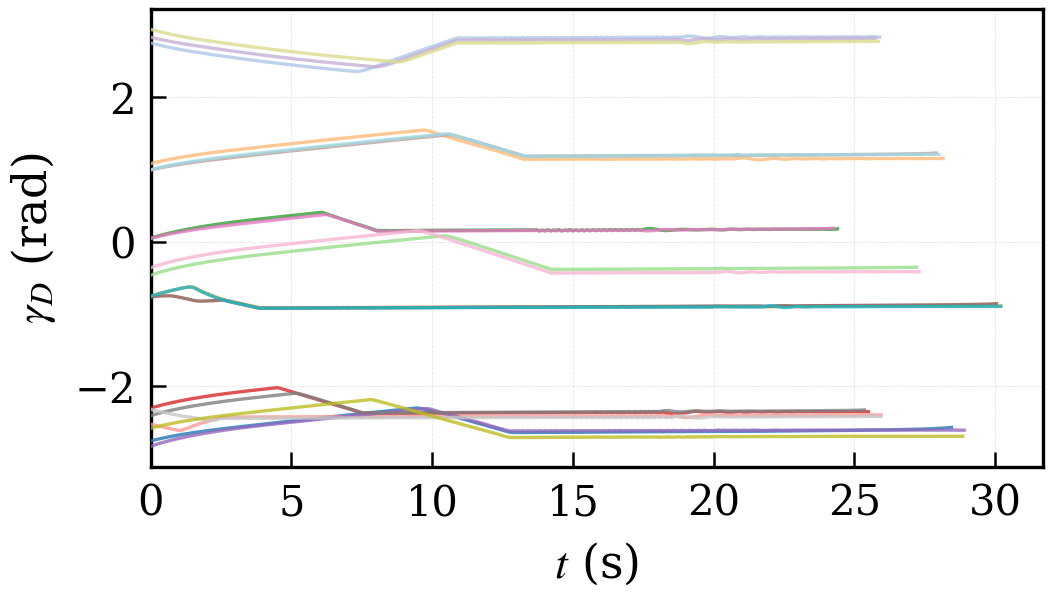
\includegraphics[width=3.0in]{mappo_nopn_heading.png}}
%DIFDELCMD < \hfil
%DIFDELCMD < \subfloat[Velocity $V_D$]{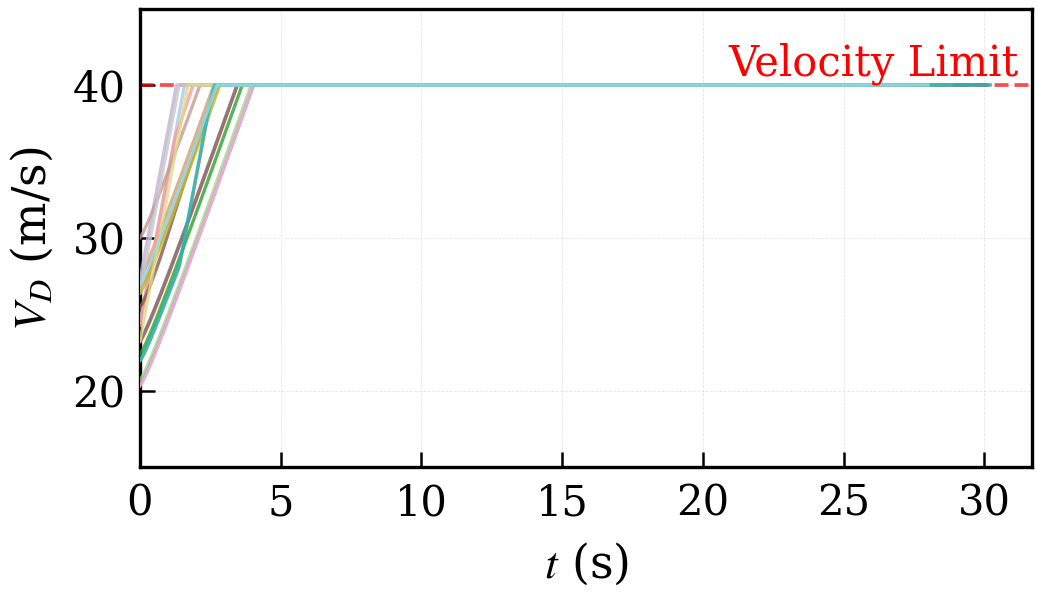
\includegraphics[width=3.0in]{mappo_nopn_velocity.png}}
%DIFDELCMD < \hfil
%DIFDELCMD < \subfloat[Axial acceleration $n_x$]{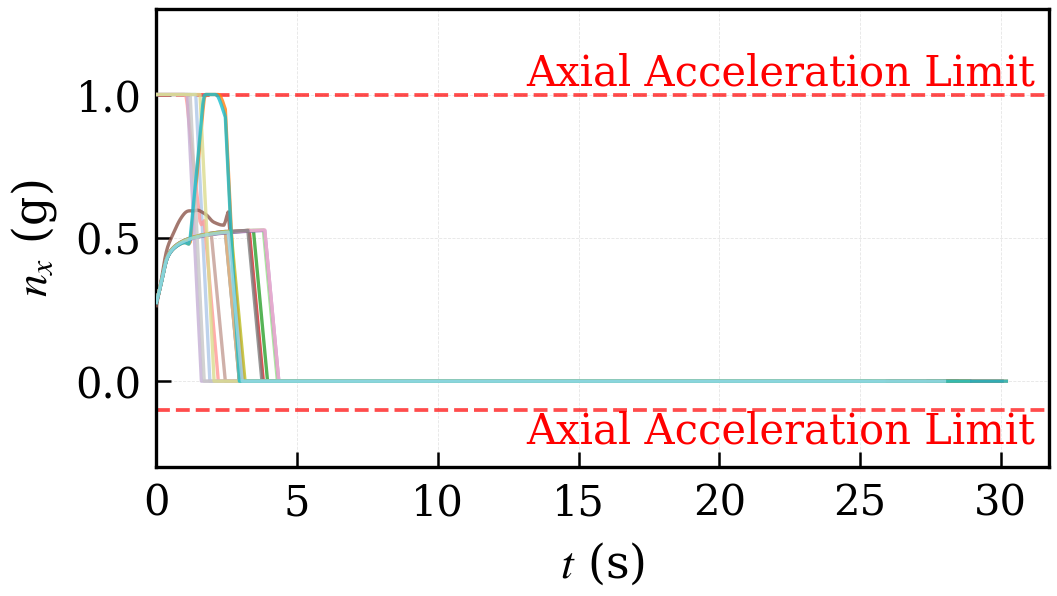
\includegraphics[width=3.0in]{mappo_nopn_nx.png}}
%DIFDELCMD < \vspace{0pt}
%DIFDELCMD < %%%
\DIFdelendFL \DIFaddbeginFL 
\includegraphics[width=6.7in]{new_sim_fig/figures_v10/mappo/standalone_duav_legend.png}\\[-2pt]
\subfloat[Axial command \(n_x\)]{
\includegraphics[width=3.30in]{new_sim_fig/figures_v10/mappo/mappo_nopn_nx.png}}\hfill
\subfloat[Yaw-plane command \(n_y\)]{
\includegraphics[width=3.30in]{new_sim_fig/figures_v10/mappo/mappo_nopn_ny.png}}\\[-2pt]
\subfloat[Pitch-plane command \(n_z\)]{
\includegraphics[width=3.30in]{new_sim_fig/figures_v10/mappo/mappo_nopn_nz.png}}\hfill
\subfloat[Speed \(V_D\)]{
\includegraphics[width=3.30in]{new_sim_fig/figures_v10/mappo/mappo_nopn_velocity.png}}\\[-2pt]
\subfloat[Yaw angle \(\psi_D\)]{
\includegraphics[width=3.30in]{new_sim_fig/figures_v10/mappo/mappo_nopn_yaw.png}}\hfill
\subfloat[Pitch angle \(\theta_D\)]{
\includegraphics[width=3.30in]{new_sim_fig/figures_v10/mappo/mappo_nopn_pitch.png}}
\DIFaddendFL \caption{\DIFdelbeginFL \DIFdelFL{Kinematic and control effort profiles of }\DIFdelendFL ART-MAPPO \DIFaddbeginFL \DIFaddFL{three-dimensional command, speed, and attitude histories
}\DIFaddendFL for Case~1. The \DIFdelbeginFL \DIFdelFL{algorithm successfully maximizes closing speed while strictly adhering to }\DIFdelendFL \DIFaddbeginFL \DIFaddFL{three command channels remain in }\DIFaddendFL the \DIFdelbeginFL \DIFdelFL{$\pm1$\,g normal overload constraint}\DIFdelendFL \DIFaddbeginFL \DIFaddFL{common constrained
envelope; yaw and pitch show the corresponding horizontal and vertical
trajectory shaping}\DIFaddendFL .}
\label{fig:case1_mappo_kine}
\DIFdelbeginFL %DIFDELCMD < \end{figure}
%DIFDELCMD < %%%
\DIFdelend \DIFaddbegin \end{figure*}
\DIFaddend 

\DIFdelbegin \DIFdel{In stark contrast, the performance of the baseline PN guidance is presented in Fig.~\ref{fig:case1_pn_traj} and }\DIFdelend Fig.~\DIFdelbegin \DIFdel{\ref{fig:case1_pn_kine}. While PN eventually intercepts the targets (Fig.~\ref{fig:case1_pn_traj}), its purely reactive nature leads to a highly inefficient pursuit strategy. As clearly depicted in Fig.~\ref{fig:case1_pn_kine}(a), the normal acceleration ($n_y$) of PN drastically diverges, severely violating the $\pm1$}\DIFdelend \DIFaddbegin \DIFadd{\ref{fig:case1_mappo_coord} completes the ART-MAPPO evidence chain. The
individual \(t_{go}\) histories approach zero in their assigned groups, the
group-relative errors collapse toward zero, and all eight terminal arrival
spreads remain below the 0.5-s synchronization criterion. The largest spread
in the selected Case~1 run is 0.25}\DIFaddend \,\DIFdelbegin \DIFdel{g physical limit because the
algorithm lacks predictive capability against evasive maneuvers, thus demanding excessive and sudden control efforts in the terminal phase. In realistic flight conditions, such catastrophic actuator saturation would inevitably result in structural damage or loss of control, rendering the interception a failure.
Consequently, the velocity decays significantly over time (}\DIFdelend \DIFaddbegin \DIFadd{s.
}

\begin{figure*}[!t]
\centering
\subfloat[Time-to-go]{
\includegraphics[width=2.25in]{new_sim_fig/figures_v10/mappo/mappo_nopn_tgo.png}}\hfill
\subfloat[Time-to-go error]{
\includegraphics[width=2.25in]{new_sim_fig/figures_v10/mappo/mappo_nopn_tgo_error.png}}\hfill
\subfloat[Terminal arrival spread]{
\includegraphics[width=2.25in]{new_sim_fig/figures_v10/mappo/mappo_nopn_time_sync.png}}
\caption{\DIFaddFL{ART-MAPPO temporal-coordination histories for Case~1. The decreasing
group-relative time-to-go errors lead to a maximum terminal spread of
0.25\,s.}}
\label{fig:case1_mappo_coord}
\end{figure*}
\FloatBarrier

\DIFadd{The capacity-matched PN reference also intercepts all assigned targets in
Case~1. }\DIFaddend Fig.~\DIFdelbegin \DIFdel{\ref{fig:case1_pn_kine}(c))
, dragging out the interceptionduration}\DIFdelend \DIFaddbegin \DIFadd{\ref{fig:case1_pn_traj} shows comparable hit times (24.35--30.30\,s)
but different reactive path shapes. Its range panel confirms that no apparent
trajectory crossing is mistaken for an interception; every paired range
reaches the 3-m hit region}\DIFaddend .

\DIFdelbegin %DIFDELCMD < \begin{figure}[!ht]
%DIFDELCMD < %%%
\DIFdelendFL \DIFaddbeginFL \begin{figure*}[!t]
\DIFaddendFL \centering
\DIFdelbeginFL %DIFDELCMD < 
\includegraphics[width=3.2in]{pn_nopn_trajectory.png}
%DIFDELCMD < %%%
\DIFdelendFL \DIFaddbeginFL \subfloat[Horizontal trajectory]{
\includegraphics[width=2.25in]{new_sim_fig/figures_v10/pn/pn_nopn_trajectory.png}}\hfill
\subfloat[Three-dimensional trajectory]{
\includegraphics[width=2.25in]{new_sim_fig/figures_v10/pn/pn_nopn_trajectory_3d.png}}\hfill
\subfloat[Interceptor--target range]{
\includegraphics[width=2.25in]{new_sim_fig/figures_v10/pn/pn_nopn_distance.png}}
\DIFaddendFL \caption{\DIFdelbeginFL \DIFdelFL{Engagement trajectories of the defending swarm using the }\DIFdelendFL \DIFaddbeginFL \DIFaddFL{Capacity-matched }\DIFaddendFL PN \DIFdelbeginFL \DIFdelFL{baseline in }\DIFdelendFL \DIFaddbeginFL \DIFaddFL{engagement geometry and range histories for
}\DIFaddendFL Case~1. \DIFaddbeginFL \DIFaddFL{Both trajectory views and the paired ranges confirm completion of all
20 assigned interceptions.}\DIFaddendFL }
\label{fig:case1_pn_traj}
\DIFdelbeginFL %DIFDELCMD < \end{figure}
%DIFDELCMD < 

%DIFDELCMD < \begin{figure}[!ht]
%DIFDELCMD < \centering
%DIFDELCMD < 
\includegraphics[width=3.0in]{standalone_duav_legend.png}
%DIFDELCMD < \subfloat[Normal acceleration $n_y$]{
\includegraphics[width=3.0in]{pn_nopn_ny.png}}
%DIFDELCMD < \hfil
%DIFDELCMD < \subfloat[Heading angle $\gamma_D$]{
\includegraphics[width=3.0in]{pn_nopn_heading.png}}
%DIFDELCMD < \hfil
%DIFDELCMD < \subfloat[Velocity $V_D$]{
\includegraphics[width=3.0in]{pn_nopn_velocity.png}}
%DIFDELCMD < \hfil
%DIFDELCMD < \subfloat[Axial acceleration $n_x$]{
\includegraphics[width=3.0in]{pn_nopn_nx.png}}
%DIFDELCMD < \vspace{0pt}
%DIFDELCMD < %%%
%DIFDELCMD < \caption{%
{%DIFAUXCMD
\DIFdelFL{Kinematic and control effort profiles of the PN baseline for Case~1, illustrating severe terminal actuator saturation ($n_y$ exceeding $\pm1$\,g limits).}}
%DIFAUXCMD
%DIFDELCMD < \label{fig:case1_pn_kine}
%DIFDELCMD < \end{figure}
%DIFDELCMD < %%%
\DIFdelend \DIFaddbegin \end{figure*}
\DIFaddend 

\DIFdelbegin \DIFdel{Beyond individual interception capabilities, a core requirement of swarm defense is the execution of a simultaneous saturation strike to prevent the targets from defeating the interceptors piecemeal. This vital temporal coordination is dynamically achieved during the flight, as evidenced by the time-to-go ($t_{go}$) profiles }\DIFdelend \DIFaddbegin \DIFadd{The PN state histories }\DIFaddend in Fig.~\DIFdelbegin \DIFdel{\ref{fig:case1_mappo_tgo}. The $t_{go}$ curves of interceptors assigned to
the same target rapidly converge as the engagement progresses. This explicitly demonstrates that ART-MAPPO actively shapes the velocity distribution of the swarm to synchronize the remaining flight times long before the actual impact}\DIFdelend \DIFaddbegin \DIFadd{\ref{fig:case1_pn_kine} provide a channel-wise
check under the same action bounds. The \(n_x\) command again raises speed to
approximately 40\,m/s. The \(n_y\) histories reveal the reactive steering
trend, whereas the independent \(n_z\) channel produces the vertical
trajectory response. Their resulting yaw courses remain continuous after
unwrapping, and pitch stays within about 0.09\,rad. The raw PN command vector
reaches the common clipping limits in all three channels, so the comparison is
capacity matched rather than an unconstrained-PN comparison}\DIFaddend .

\DIFdelbegin %DIFDELCMD < \begin{figure}[!ht]
%DIFDELCMD < %%%
\DIFdelendFL \DIFaddbeginFL \begin{figure*}[!t]
\DIFaddendFL \centering
\DIFdelbeginFL %DIFDELCMD < 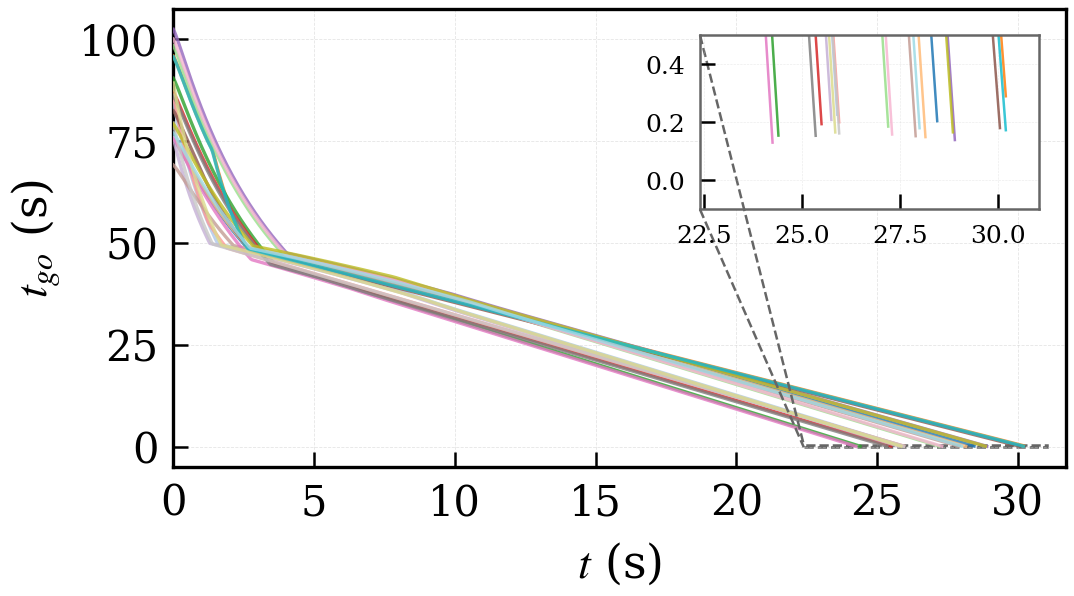
\includegraphics[width=3.2in]{mappo_nopn_tgo.png}
%DIFDELCMD < %%%
\DIFdelendFL \DIFaddbeginFL \subfloat[Axial command \(n_x\)]{
\includegraphics[width=3.30in]{new_sim_fig/figures_v10/pn/pn_nopn_nx.png}}\hfill
\subfloat[Yaw-plane command \(n_y\)]{
\includegraphics[width=3.30in]{new_sim_fig/figures_v10/pn/pn_nopn_ny.png}}\\[-2pt]
\subfloat[Pitch-plane command \(n_z\)]{
\includegraphics[width=3.30in]{new_sim_fig/figures_v10/pn/pn_nopn_nz.png}}\hfill
\subfloat[Speed \(V_D\)]{
\includegraphics[width=3.30in]{new_sim_fig/figures_v10/pn/pn_nopn_velocity.png}}\\[-2pt]
\subfloat[Yaw angle \(\psi_D\)]{
\includegraphics[width=3.30in]{new_sim_fig/figures_v10/pn/pn_nopn_yaw.png}}\hfill
\subfloat[Pitch angle \(\theta_D\)]{
\includegraphics[width=3.30in]{new_sim_fig/figures_v10/pn/pn_nopn_pitch.png}}
\DIFaddendFL \caption{\DIFdelbeginFL \DIFdelFL{Time-to-go ($t_{go}$) profiles of the defending swarm using ART-MAPPO in }\DIFdelendFL \DIFaddbeginFL \DIFaddFL{Capacity-matched PN three-dimensional command, speed, and attitude
histories for }\DIFaddendFL Case~1. \DIFdelbeginFL \DIFdelFL{Interceptors assigned to }\DIFdelendFL \DIFaddbeginFL \DIFaddFL{The panels show the reactive steering solution under
}\DIFaddendFL the same \DIFdelbeginFL \DIFdelFL{target actively synchronize their remaining flight times to guarantee a simultaneous saturation strike}\DIFdelendFL \DIFaddbeginFL \DIFaddFL{\(n_x\), \(n_y\), and \(n_z\) bounds used by ART-MAPPO}\DIFaddendFL .}
\DIFdelbeginFL %DIFDELCMD < \label{fig:case1_mappo_tgo}
%DIFDELCMD < \end{figure}
%DIFDELCMD < %%%
\DIFdelend \DIFaddbegin \label{fig:case1_pn_kine}
\end{figure*}
\DIFaddend 

\DIFdelbegin \DIFdel{Consequently, }\DIFdelend \DIFaddbegin \DIFadd{The PN \(t_{go}\) and group-relative errors in }\DIFaddend Fig.~\DIFdelbegin \DIFdel{\ref{fig:case1_time_sync} explicitly validates the ultimate temporal coordination capability by displaying the terminal arrival time difference ($\Delta t$) among the interceptors assigned to each respective target group. The maximum $\Delta t$ across all eight coordinated groups is remarkably tight, bounded to merely 0.45}\DIFdelend \DIFaddbegin \DIFadd{\ref{fig:case1_pn_coord}
also converge in this selected successful run. Its maximum terminal group
spread is 0.40\,s, compared with 0.25}\DIFaddend \,s \DIFdelbegin \DIFdel{. This quantitatively proves that the proposed framework perfectly bridges the target assignment and the trust-modulated exploration mechanisms, ensuring a strictly temporally coordinated saturation strike against the swarm threat}\DIFdelend \DIFaddbegin \DIFadd{for ART-MAPPO. Both satisfy the 0.5-s
criterion; the result demonstrates feasibility and a tighter ART-MAPPO timing
outcome for this representative initialization, not a population-level claim}\DIFaddend .

\DIFdelbegin %DIFDELCMD < \begin{figure}[!ht]
%DIFDELCMD < %%%
\DIFdelendFL \DIFaddbeginFL \begin{figure*}[!t]
\DIFaddendFL \centering
\DIFdelbeginFL %DIFDELCMD < 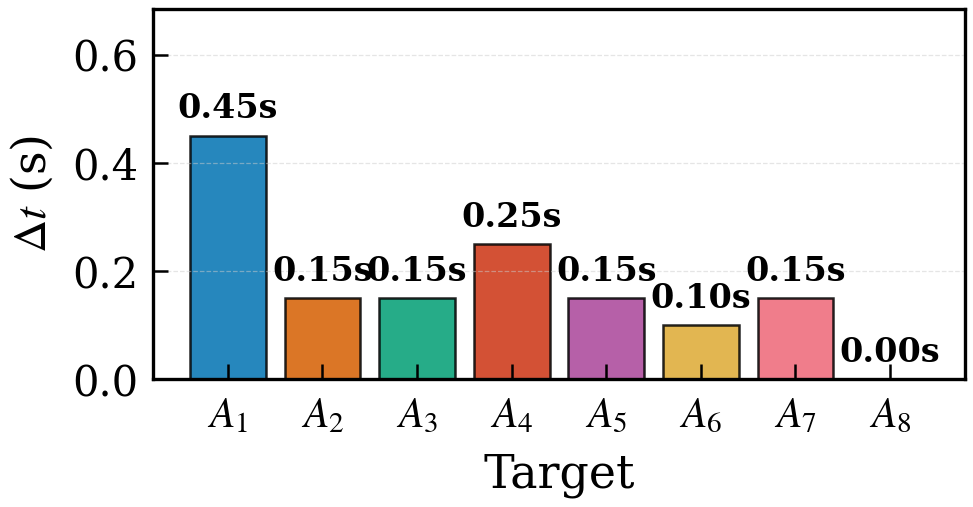
\includegraphics[width=3.0in]{mappo_success_nopn_time_sync.png}
%DIFDELCMD < %%%
\DIFdelendFL \DIFaddbeginFL \subfloat[Time-to-go]{
\includegraphics[width=2.25in]{new_sim_fig/figures_v10/pn/pn_nopn_tgo.png}}\hfill
\subfloat[Time-to-go error]{
\includegraphics[width=2.25in]{new_sim_fig/figures_v10/pn/pn_nopn_tgo_error.png}}\hfill
\subfloat[Terminal arrival spread]{
\includegraphics[width=2.25in]{new_sim_fig/figures_v10/pn/pn_nopn_time_sync.png}}
\DIFaddendFL \caption{\DIFdelbeginFL \DIFdelFL{Terminal arrival time differences $\Delta t$ within each coordinated interceptor group under ART-MAPPO. }\DIFdelendFL \DIFaddbeginFL \DIFaddFL{Capacity-matched PN temporal-coordination histories for Case~1. }\DIFaddendFL The
\DIFdelbeginFL \DIFdelFL{near-zero $\Delta t$ values explicitly validate the successful execution }\DIFdelendFL \DIFaddbeginFL \DIFaddFL{selected run attains a maximum group arrival spread }\DIFaddendFL of \DIFdelbeginFL \DIFdelFL{temporally synchronized saturation strikes}\DIFdelendFL \DIFaddbeginFL \DIFaddFL{0.40\,s}\DIFaddendFL .}
\DIFdelbeginFL %DIFDELCMD < \label{fig:case1_time_sync}
%DIFDELCMD < \end{figure}
%DIFDELCMD < %%%
\DIFdelend \DIFaddbegin \label{fig:case1_pn_coord}
\end{figure*}
\FloatBarrier
\DIFaddend 

\subsubsection{Case~2: Interception against Continuous Weaving Targets}

This scenario evaluates the \DIFdelbegin \DIFdel{robustness of the proposed }\DIFdelend framework against the sinusoidal penetration
maneuver~\cite{Zarchan1995969}, which \DIFdelbegin \DIFdel{represents a highly agile and continuous weaving threat. Such maneuvers induce high-frequency oscillations in the line-of-sight (LOS) rate, severely challenging both the guidance stability and
the temporal coordination of the defending swarm. }%DIFDELCMD < 

%DIFDELCMD < %%%
\DIFdel{The 2D engagement trajectories of the ART-MAPPO defending swarm are illustrated in }\DIFdelend \DIFaddbegin \DIFadd{continuously perturbs both horizontal and
vertical LOS geometry. }\DIFaddend Fig.~\ref{fig:case2_mappo_traj} \DIFdelbegin \DIFdel{. Despite the continuous lateral oscillations of the $A_{\text{UAV}}$, }\DIFdelend \DIFaddbegin \DIFadd{shows that }\DIFaddend ART-MAPPO
\DIFdelbegin \DIFdel{explicitly predicts and accommodates the target'sweaving motion. The defending swarm maintains all eight coordinated combat units and successfully intercepts every target with smooth pursuit curves}\DIFdelend \DIFaddbegin \DIFadd{preserves all eight assigned groups under this weaving motion. Seventeen
interceptors hit between 24.65 and 29.15\,s, and the longest group closes at
37.25\,s. The range panel verifies closure for this delayed trajectory rather
than inferring success from its projected path alone}\DIFaddend .

\DIFdelbegin %DIFDELCMD < \begin{figure}[!ht]
%DIFDELCMD < %%%
\DIFdelendFL \DIFaddbeginFL \begin{figure*}[!t]
\DIFaddendFL \centering
\DIFdelbeginFL %DIFDELCMD < 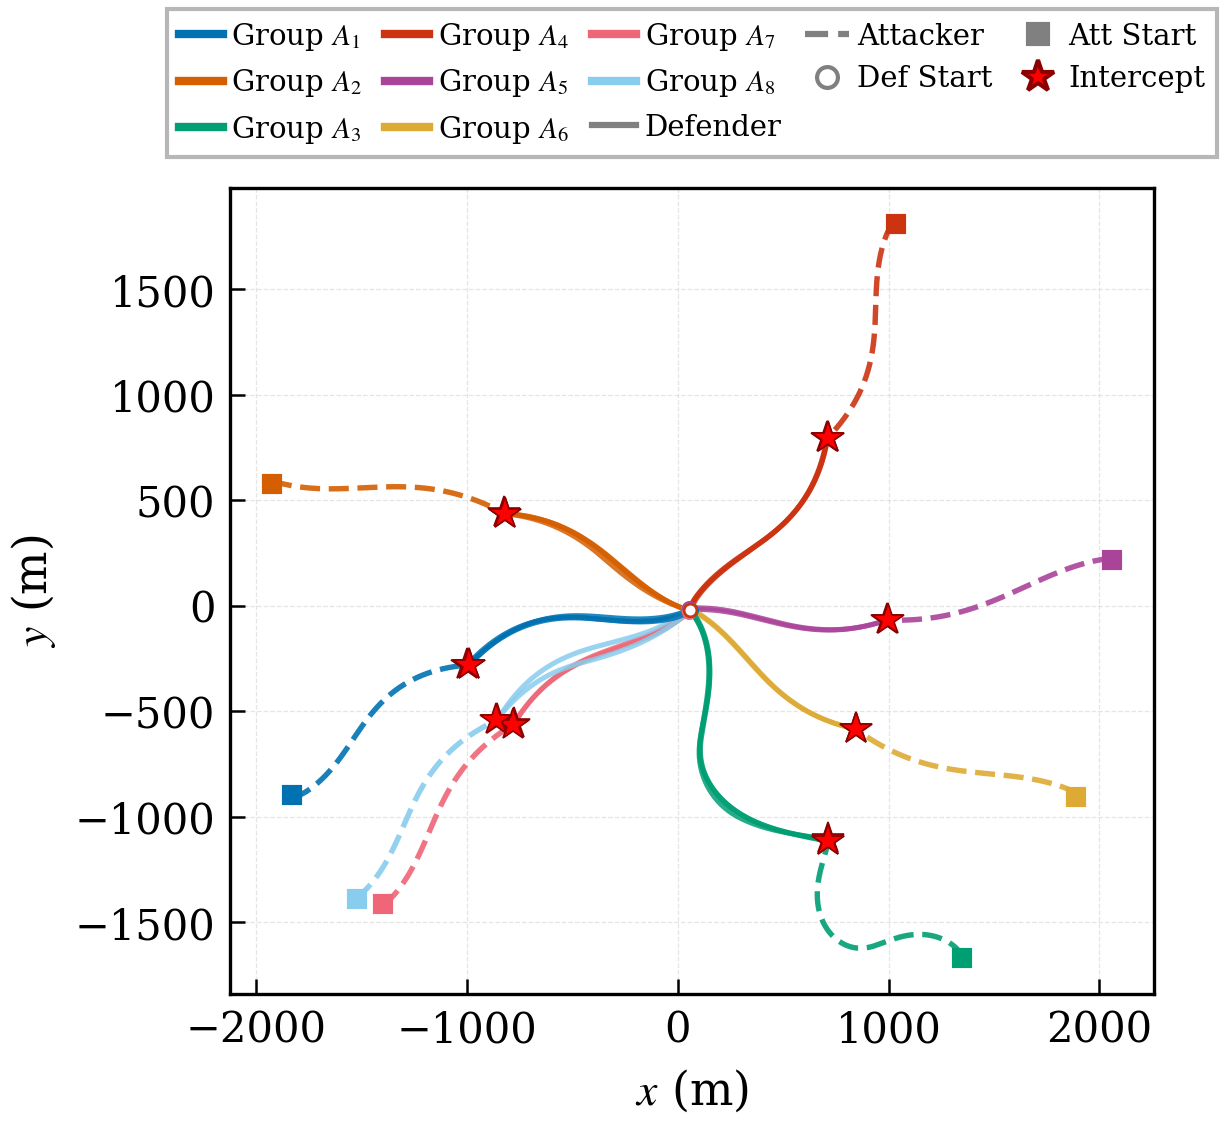
\includegraphics[width=3.2in]{mappo_sin_trajectory.png}
%DIFDELCMD < %%%
\DIFdelendFL \DIFaddbeginFL \subfloat[Horizontal trajectory]{
\includegraphics[width=2.25in]{new_sim_fig/figures_v10/mappo/mappo_sin_trajectory.png}}\hfill
\subfloat[Three-dimensional trajectory]{
\includegraphics[width=2.25in]{new_sim_fig/figures_v10/mappo/mappo_sin_trajectory_3d.png}}\hfill
\subfloat[Interceptor--target range]{
\includegraphics[width=2.25in]{new_sim_fig/figures_v10/mappo/mappo_sin_distance.png}}
\DIFaddendFL \caption{\DIFdelbeginFL \DIFdelFL{Engagement trajectories of the defending swarm using }\DIFdelendFL ART-MAPPO \DIFdelbeginFL \DIFdelFL{against }\DIFdelendFL \DIFaddbeginFL \DIFaddFL{engagement geometry and range histories for the }\DIFaddendFL continuous
weaving targets \DIFdelbeginFL \DIFdelFL{(}\DIFdelendFL \DIFaddbeginFL \DIFaddFL{in }\DIFaddendFL Case~\DIFdelbeginFL \DIFdelFL{2)}\DIFdelendFL \DIFaddbeginFL \DIFaddFL{2. The paired ranges confirm interception of both the
main cluster and the longer-duration trajectory}\DIFaddendFL .}
\label{fig:case2_mappo_traj}
\DIFdelbeginFL %DIFDELCMD < \end{figure}
%DIFDELCMD < %%%
\DIFdelend \DIFaddbegin \end{figure*}
\DIFaddend 

\DIFdelbegin \DIFdel{The underlying kinematic and control mechanisms of ART-MAPPO are further detailed in }\DIFdelend Fig.~\ref{fig:case2_mappo_kine} \DIFdelbegin \DIFdel{. The most significant advantage is observed in the normal acceleration profile ($n_y$) shown in Fig.~\ref{fig:case2_mappo_kine}(a). To counter the weaving target, ART-MAPPO generates an intelligent, adaptive oscillatory $n_y$ command that perfectly tracks the target's maneuvering frequency. Most importantly, it achieves this dynamic tracking while strictly remaining within the safe aerodynamic envelope ($\pm 1$}\DIFdelend \DIFaddbegin \DIFadd{explains how this geometry is generated. The
policy uses both normal channels: \(n_y\) responds to horizontal weaving and
\(n_z\) shapes the vertical closure, while \(n_x\) drives the defenders to the
40-m/s ceiling. The explicit yaw curves show continuous course evolution after
angle unwrapping. Pitch remains within approximately \(-0.01\) to 0.14}\DIFaddend \,\DIFdelbegin \DIFdel{g),
completely averting terminal saturation. Furthermore, it smoothly adjusts its heading angle (Fig. ~\ref{fig:case2_mappo_kine}(b)).
Similar to Case~1, ART-MAPPO aggressively leverages its axial acceleration ($n_x$) to maximize approach velocity, as demonstrated in the velocity and axial acceleration profiles (Fig.~\ref{fig:case2_mappo_kine}(c) and
(d)). }\DIFdelend \DIFaddbegin \DIFadd{rad,
which is consistent with the moderate 51--64-m terminal altitude. The raw
maximum command vector \([1.0000,1.0000,0.7749]\) remains in the common
three-dimensional action envelope.
}\DIFaddend 

\DIFdelbegin %DIFDELCMD < \begin{figure}[!ht]
%DIFDELCMD < %%%
\DIFdelendFL \DIFaddbeginFL \begin{figure*}[!t]
\DIFaddendFL \centering
\DIFdelbeginFL %DIFDELCMD < 
\includegraphics[width=3.0in]{standalone_duav_legend.png}
%DIFDELCMD < \subfloat[Normal acceleration $n_y$]{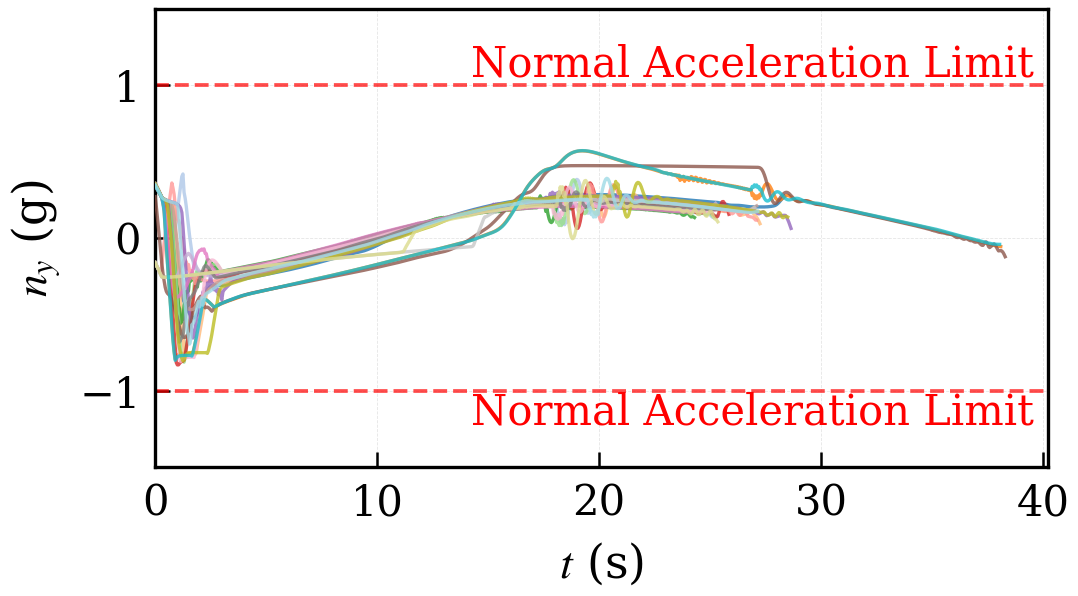
\includegraphics[width=3.0in]{mappo_sin_ny.png}}
%DIFDELCMD < \hfil
%DIFDELCMD < \subfloat[Heading angle $\gamma_D$]{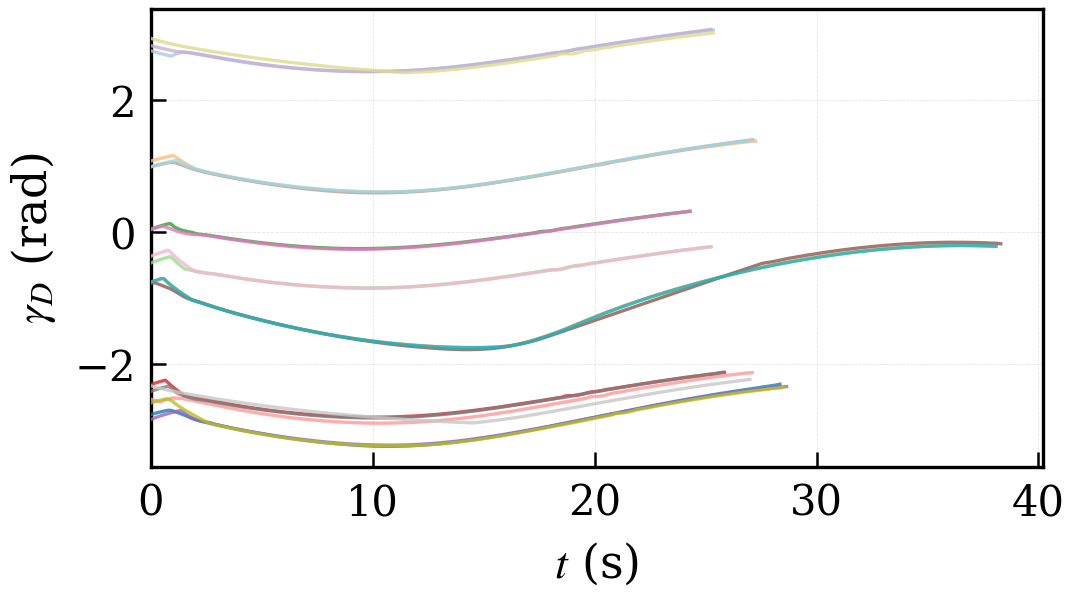
\includegraphics[width=3.0in]{mappo_sin_heading.png}}
%DIFDELCMD < \hfil
%DIFDELCMD < \subfloat[Velocity $V_D$]{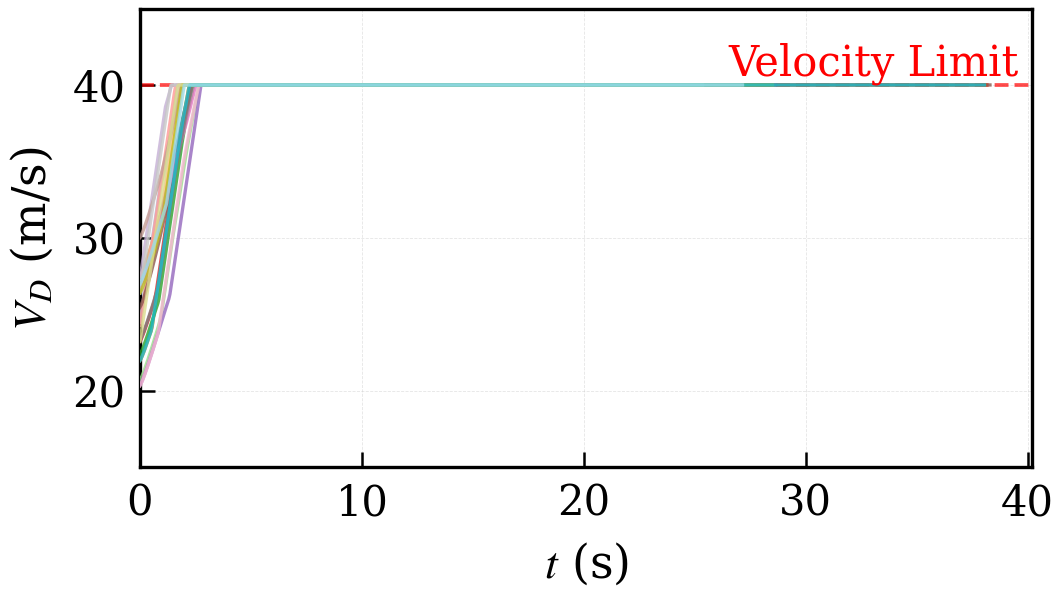
\includegraphics[width=3.0in]{mappo_sin_velocity.png}}
%DIFDELCMD < \hfil
%DIFDELCMD < \subfloat[Axial acceleration $n_x$]{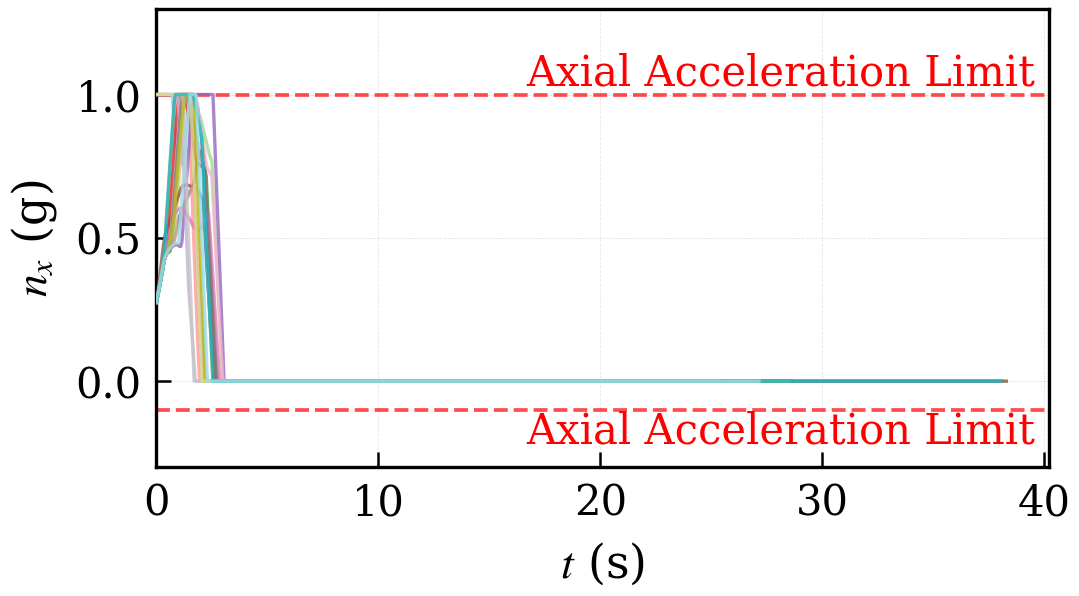
\includegraphics[width=3.0in]{mappo_sin_nx.png}}
%DIFDELCMD < \vspace{0pt}
%DIFDELCMD < %%%
%DIFDELCMD < \caption{%
{%DIFAUXCMD
\DIFdelFL{Kinematic and control effort profiles of ART-MAPPO for Case~2. The policy dynamically outputs adaptive oscillatory normal commands ($n_y$) to track the weaving target without violating the $\pm1$\,g limit.}}
%DIFAUXCMD
\DIFdelendFL \DIFaddbeginFL \subfloat[Axial command \(n_x\)]{
\includegraphics[width=3.30in]{new_sim_fig/figures_v10/mappo/mappo_sin_nx.png}}\hfill
\subfloat[Yaw-plane command \(n_y\)]{
\includegraphics[width=3.30in]{new_sim_fig/figures_v10/mappo/mappo_sin_ny.png}}\\[-2pt]
\subfloat[Pitch-plane command \(n_z\)]{
\includegraphics[width=3.30in]{new_sim_fig/figures_v10/mappo/mappo_sin_nz.png}}\hfill
\subfloat[Speed \(V_D\)]{
\includegraphics[width=3.30in]{new_sim_fig/figures_v10/mappo/mappo_sin_velocity.png}}\\[-2pt]
\subfloat[Yaw angle \(\psi_D\)]{
\includegraphics[width=3.30in]{new_sim_fig/figures_v10/mappo/mappo_sin_yaw.png}}\hfill
\subfloat[Pitch angle \(\theta_D\)]{
\includegraphics[width=3.30in]{new_sim_fig/figures_v10/mappo/mappo_sin_pitch.png}}
\caption{\DIFaddFL{ART-MAPPO three-dimensional command, speed, and attitude histories
for Case~2. The two normal-command channels accommodate the horizontal and
vertical components of the continuous weaving engagement.}}
\DIFaddendFL \label{fig:case2_mappo_kine}
\DIFdelbeginFL %DIFDELCMD < \end{figure}
%DIFDELCMD < %%%
\DIFdelend \DIFaddbegin \end{figure*}
\DIFaddend 

\DIFdelbegin \DIFdel{Conversely, the PN baseline completely fails to handle the high-frequency dynamic engagementgeometry.
}\DIFdelend The \DIFdelbegin \DIFdel{reactive nature of PN results in phase-lagged trajectories that struggle to close the distance (}\DIFdelend \DIFaddbegin \DIFadd{ART-MAPPO coordination panels in }\DIFaddend Fig.~\DIFdelbegin \DIFdel{\ref{fig:case2_pn_traj}). As revealed in the
control profiles (}\DIFdelend \DIFaddbegin \DIFadd{\ref{fig:case2_mappo_coord} show
that the time-to-go errors recover from the weaving-induced transients and
converge within each assigned group. All eight group spreads remain below
0.5\,s, and the largest is 0.30\,s despite the 37-s outlying engagement.
}

\begin{figure*}[!t]
\centering
\subfloat[Time-to-go]{
\includegraphics[width=2.25in]{new_sim_fig/figures_v10/mappo/mappo_sin_tgo.png}}\hfill
\subfloat[Time-to-go error]{
\includegraphics[width=2.25in]{new_sim_fig/figures_v10/mappo/mappo_sin_tgo_error.png}}\hfill
\subfloat[Terminal arrival spread]{
\includegraphics[width=2.25in]{new_sim_fig/figures_v10/mappo/mappo_sin_time_sync.png}}
\caption{\DIFaddFL{ART-MAPPO temporal-coordination histories for Case~2. Coordination
is retained under continuous weaving, with a maximum group spread of
0.30\,s.}}
\label{fig:case2_mappo_coord}
\end{figure*}
\FloatBarrier

\DIFadd{The constrained PN reference also completes the selected Case~2 engagement.
}\DIFaddend Fig.~\DIFdelbegin \DIFdel{\ref{fig:case2_pn_kine}), the PN guidance law suffers from catastrophic actuator saturation during the terminal phase. Specifically, the normal commands ($n_y$) frequently breach the $\pm 1$}\DIFdelend \DIFaddbegin \DIFadd{\ref{fig:case2_pn_traj} shows a similar main interception cluster and a
longer trajectory that terminates at 36.90}\DIFaddend \,\DIFdelbegin \DIFdel{g limit (Fig. ~\ref{fig:case2_pn_kine}(a)), which would severely compromise flight safety and render the interception a failure in real-world applications.
}\DIFdelend \DIFaddbegin \DIFadd{s. The 3-D paths reflect the
reactive response to the varying LOS, while the range histories verify all 20
hits in this particular run.
}\DIFaddend 

\DIFdelbegin %DIFDELCMD < \begin{figure}[!ht]
%DIFDELCMD < %%%
\DIFdelendFL \DIFaddbeginFL \begin{figure*}[!t]
\DIFaddendFL \centering
\DIFdelbeginFL %DIFDELCMD < 
\includegraphics[width=3.2in]{pn_sin_trajectory.png}
%DIFDELCMD < %%%
%DIFDELCMD < \caption{%
{%DIFAUXCMD
\DIFdelFL{Engagement trajectories of the defending swarm using the PN baseline in Case~2.}}
%DIFAUXCMD
\DIFdelendFL \DIFaddbeginFL \subfloat[Horizontal trajectory]{
\includegraphics[width=2.25in]{new_sim_fig/figures_v10/pn/pn_sin_trajectory.png}}\hfill
\subfloat[Three-dimensional trajectory]{
\includegraphics[width=2.25in]{new_sim_fig/figures_v10/pn/pn_sin_trajectory_3d.png}}\hfill
\subfloat[Interceptor--target range]{
\includegraphics[width=2.25in]{new_sim_fig/figures_v10/pn/pn_sin_distance.png}}
\caption{\DIFaddFL{Capacity-matched PN engagement geometry and range histories for
Case~2. The range panel confirms closure of the long-duration engagement near
37\,s.}}
\DIFaddendFL \label{fig:case2_pn_traj}
\DIFdelbeginFL %DIFDELCMD < \end{figure}
%DIFDELCMD < %%%
\DIFdelend \DIFaddbegin \end{figure*}
\DIFaddend 

\DIFdelbegin %DIFDELCMD < \begin{figure}[!ht]
%DIFDELCMD < %%%
\DIFdelendFL \DIFaddbeginFL \DIFaddFL{Fig.~\ref{fig:case2_pn_kine} shows that PN uses more of the available
yaw-plane maneuver envelope in the difficult weaving geometry. The \(n_y\)
histories exhibit sustained use of the available yaw-plane authority, and the
recorded command reaches the \(\pm1g\) bound. The independent \(n_z\) channel
shows the corresponding vertical response. Together with the yaw and pitch
panels, these curves
confirm that the PN comparison uses a genuinely three-dimensional, bounded
guidance implementation rather than a planar surrogate.
}

\begin{figure*}[!t]
\DIFaddendFL \centering
\DIFdelbeginFL %DIFDELCMD < 
\includegraphics[width=3.0in]{standalone_duav_legend.png}
%DIFDELCMD < \subfloat[Normal acceleration $n_y$]{
\includegraphics[width=3.0in]{pn_sin_ny.png}}
%DIFDELCMD < \hfil
%DIFDELCMD < \subfloat[Heading angle $\gamma_D$]{
\includegraphics[width=3.0in]{pn_sin_heading.png}}
%DIFDELCMD < \hfil
%DIFDELCMD < \subfloat[Velocity $V_D$]{
\includegraphics[width=3.0in]{pn_sin_velocity.png}}
%DIFDELCMD < \hfil
%DIFDELCMD < \subfloat[Axial acceleration $n_x$]{
\includegraphics[width=3.0in]{pn_sin_nx.png}}
%DIFDELCMD < \vspace{0pt}
%DIFDELCMD < %%%
\DIFdelendFL \DIFaddbeginFL \subfloat[Axial command \(n_x\)]{
\includegraphics[width=3.30in]{new_sim_fig/figures_v10/pn/pn_sin_nx.png}}\hfill
\subfloat[Yaw-plane command \(n_y\)]{
\includegraphics[width=3.30in]{new_sim_fig/figures_v10/pn/pn_sin_ny.png}}\\[-2pt]
\subfloat[Pitch-plane command \(n_z\)]{
\includegraphics[width=3.30in]{new_sim_fig/figures_v10/pn/pn_sin_nz.png}}\hfill
\subfloat[Speed \(V_D\)]{
\includegraphics[width=3.30in]{new_sim_fig/figures_v10/pn/pn_sin_velocity.png}}\\[-2pt]
\subfloat[Yaw angle \(\psi_D\)]{
\includegraphics[width=3.30in]{new_sim_fig/figures_v10/pn/pn_sin_yaw.png}}\hfill
\subfloat[Pitch angle \(\theta_D\)]{
\includegraphics[width=3.30in]{new_sim_fig/figures_v10/pn/pn_sin_pitch.png}}
\DIFaddendFL \caption{\DIFdelbeginFL \DIFdelFL{Kinematic and control effort profiles of the }\DIFdelendFL \DIFaddbeginFL \DIFaddFL{Capacity-matched }\DIFaddendFL PN \DIFdelbeginFL \DIFdelFL{baseline }\DIFdelendFL \DIFaddbeginFL \DIFaddFL{three-dimensional command, speed, and attitude
histories }\DIFaddendFL for Case~\DIFdelbeginFL \DIFdelFL{2, highlighting catastrophic terminal actuator saturation ($n_y$ significantly exceeding limits)}\DIFdelendFL \DIFaddbeginFL \DIFaddFL{2. The yaw-plane command makes sustained use of the common
maneuver envelope while the separate \(n_z\) channel shapes vertical motion}\DIFaddendFL .}
\label{fig:case2_pn_kine}
\DIFdelbeginFL %DIFDELCMD < \end{figure}
%DIFDELCMD < %%%
\DIFdelend \DIFaddbegin \end{figure*}
\FloatBarrier
\DIFaddend 

The \DIFdelbegin \DIFdel{continuous maneuvering of the targets also disrupts conventional coordination mechanisms. However, this vital temporal synchronization is dynamically sustained by ART-MAPPO during the flight, as evidenced by the time-to-go ($t_{go}$) profiles }\DIFdelend \DIFaddbegin \DIFadd{corresponding PN coordination curves }\DIFaddend in Fig.~\DIFdelbegin \DIFdel{\ref{fig:case2_mappo_tgo}. Even against severe LOS oscillations, the $t_{go}$ curves of interceptors assigned to the same target smoothly converge . This demonstrates that the algorithm continuously and intelligently adapts the swarm'svelocity distribution to lock in synchronized impact times, despite the highly dynamic nature of the weaving threats}\DIFdelend \DIFaddbegin \DIFadd{\ref{fig:case2_pn_coord}
also converge for all eight groups in the selected successful run. Its maximum
arrival spread is 0.35\,s, 0.05\,s above the ART-MAPPO value but still below
the 0.5-s criterion. The Monte Carlo comparison that follows is used for
method-level reliability conclusions across randomized conditions}\DIFaddend .

\DIFdelbegin %DIFDELCMD < \begin{figure}[!ht]
%DIFDELCMD < %%%
\DIFdelendFL \DIFaddbeginFL \begin{figure*}[!t]
\DIFaddendFL \centering
\DIFdelbeginFL %DIFDELCMD < 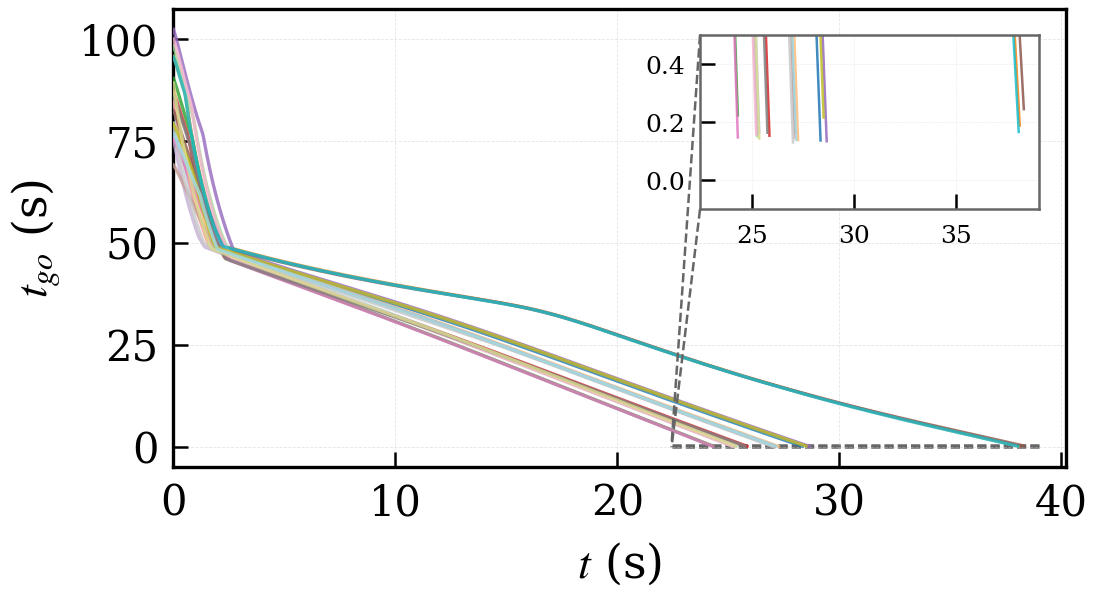
\includegraphics[width=3.2in]{mappo_sin_tgo.png}
%DIFDELCMD < %%%
\DIFdelendFL \DIFaddbeginFL \subfloat[Time-to-go]{
\includegraphics[width=2.25in]{new_sim_fig/figures_v10/pn/pn_sin_tgo.png}}\hfill
\subfloat[Time-to-go error]{
\includegraphics[width=2.25in]{new_sim_fig/figures_v10/pn/pn_sin_tgo_error.png}}\hfill
\subfloat[Terminal arrival spread]{
\includegraphics[width=2.25in]{new_sim_fig/figures_v10/pn/pn_sin_time_sync.png}}
\DIFaddendFL \caption{\DIFdelbeginFL \DIFdelFL{Time-to-go ($t_{go}$) profiles of the defending swarm using ART-MAPPO in }\DIFdelendFL \DIFaddbeginFL \DIFaddFL{Capacity-matched PN temporal-coordination histories for }\DIFaddendFL Case~2. \DIFdelbeginFL \DIFdelFL{Interceptors actively synchronize their remaining flight times despite the continuous high-G maneuvers }\DIFdelendFL \DIFaddbeginFL \DIFaddFL{The
selected run attains a maximum group arrival spread }\DIFaddendFL of \DIFdelbeginFL \DIFdelFL{the targets}\DIFdelendFL \DIFaddbeginFL \DIFaddFL{0.35\,s}\DIFaddendFL .}
\DIFdelbeginFL %DIFDELCMD < \label{fig:case2_mappo_tgo}
%DIFDELCMD < \end{figure}
%DIFDELCMD < %%%
\DIFdelend \DIFaddbegin \label{fig:case2_pn_coord}
\end{figure*}
\FloatBarrier
\DIFaddend 

\DIFdelbegin \DIFdel{Consequently, the ultimate validation of }\DIFdelend \DIFaddbegin \begin{table}[H]
\centering
\caption{\DIFaddFL{Representative Three-Dimensional Engagement Results}}
\label{tab:representative_cases}
\scriptsize
\setlength{\tabcolsep}{2.5pt}
\begin{tabular}{lccccc}
\toprule
\DIFaddFL{Method }& \DIFaddFL{Case }& \DIFaddFL{Hits }& \DIFaddFL{Targets }& \DIFaddFL{Sync }& \DIFaddFL{Spread (s) }\\
\midrule
\DIFaddendFL ART-MAPPO \DIFdelbeginFL \DIFdelFL{'s saturation strike capability under extreme dynamic conditions is explicitly presented in Fig.~\ref{fig:case2_time_sync}. Even against highly evasive sinusoidal targets, the maximum terminal arrival time difference ($\Delta t$) among the coordinated groups is strictly bounded to }\DIFdelendFL \DIFaddbeginFL & \DIFaddFL{1 }& \DIFaddFL{20/20 }& \DIFaddFL{8/8 }& \DIFaddFL{8/8 }& \DIFaddFL{0.25 }\\
\DIFaddFL{PN (\(N=4\)) }& \DIFaddFL{1 }& \DIFaddFL{20/20 }& \DIFaddFL{8/8 }& \DIFaddFL{8/8 }& \DIFaddFL{0.40 }\\
\DIFaddFL{ART-MAPPO }& \DIFaddFL{2 }& \DIFaddFL{20/20 }& \DIFaddFL{8/8 }& \DIFaddFL{8/8 }& \DIFaddendFL 0.30 \DIFdelbeginFL \DIFdelFL{\,s. This exceptional synchronization quantitatively confirms the superiority of the }\DIFdelendFL \DIFaddbeginFL \\
\DIFaddFL{PN (\(N=4\)) }& \DIFaddFL{2 }& \DIFaddFL{20/20 }& \DIFaddFL{8/8 }& \DIFaddFL{8/8 }& \DIFaddFL{0.35 }\\
\bottomrule
\end{tabular}
\end{table}

\DIFadd{Table~\ref{tab:representative_cases} summarizes the four plotted runs. All
saved impacts satisfy the 3-m hit criterion. From the recorded commands,
}\DIFaddend ART-MAPPO\DIFdelbegin \DIFdel{framework in executing temporally coordinated saturation strikes in highly complex adversarial environments}\DIFdelend \DIFaddbegin \DIFadd{'s maximum command magnitudes \([|n_x|,|n_y|,|n_z|]\) are
\([0.9882,0.9975,0.6061]\) in Case~1 and
\([1.0000,1.0000,0.7749]\) in Case~2. PN reaches the common
\([1,1,1]\) clipping vector in both cases. Thus, the representative curves
establish four feasible bounded engagements, while the Monte Carlo results
below provide the appropriate basis for comparing reliability}\DIFaddend .

\DIFdelbegin %DIFDELCMD < \begin{figure}[!ht]
%DIFDELCMD < \centering
%DIFDELCMD < 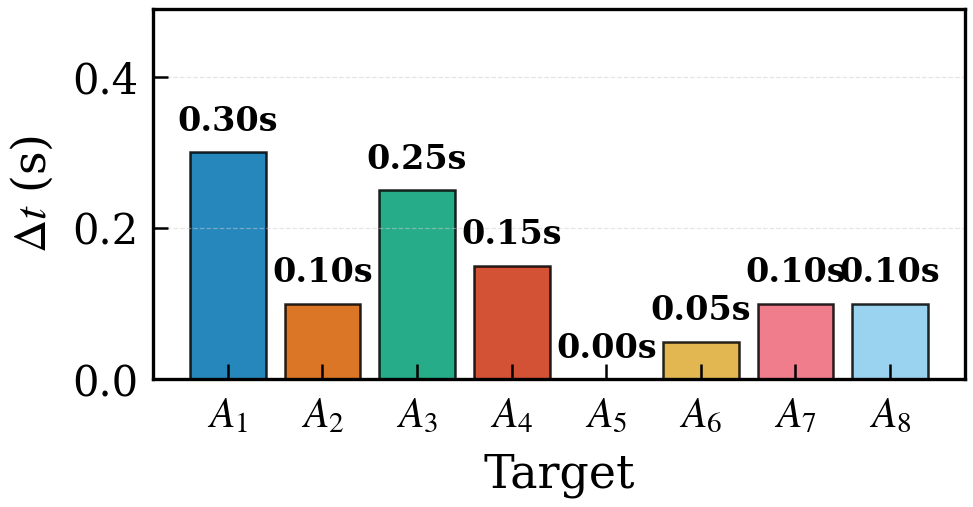
\includegraphics[width=3.0in]{mappo_success_sin_time_sync.png}
%DIFDELCMD < %%%
%DIFDELCMD < \caption{%
{%DIFAUXCMD
\DIFdelFL{Terminal arrival time differences $\Delta t$ for Case~2. The remarkably low variance ($\le 0.30$\,s) proves that ART-MAPPO preserves strict temporal synchronization even against continuous weaving targets.}}
%DIFAUXCMD
%DIFDELCMD < \label{fig:case2_time_sync}
%DIFDELCMD < \end{figure}
%DIFDELCMD < 

%DIFDELCMD < %%%
\DIFdelend \subsection{Monte Carlo Statistical Analysis and Robustness}
\label{subsec:montecarlo}

To rigorously quantify the robustness of the proposed framework, 1000 independent Monte Carlo trials are conducted for each case. It is important to note that the statistical distributions presented in Fig.~\ref{fig:mc_boxplots} ($E_{co\text{-}time}$, $E_n$, $E_{miss}$, and $E_t$) are exclusively derived from the successful interception trials. Specifically, out of the 1000 trials in Case~1, ART-MAPPO and PN successfully intercepted the targets 987 and 944 times, respectively. In the highly dynamic Case~2, ART-MAPPO maintained a remarkable 971 successful interceptions, whereas the baseline PN succeeded only 175 times. 

\DIFdelbegin %DIFDELCMD < \begin{figure}[!t]
%DIFDELCMD < %%%
\DIFdelendFL \DIFaddbeginFL \begin{figure}[H]
\DIFaddendFL \centering
\DIFdelbeginFL %DIFDELCMD < \subfloat[Case~1]{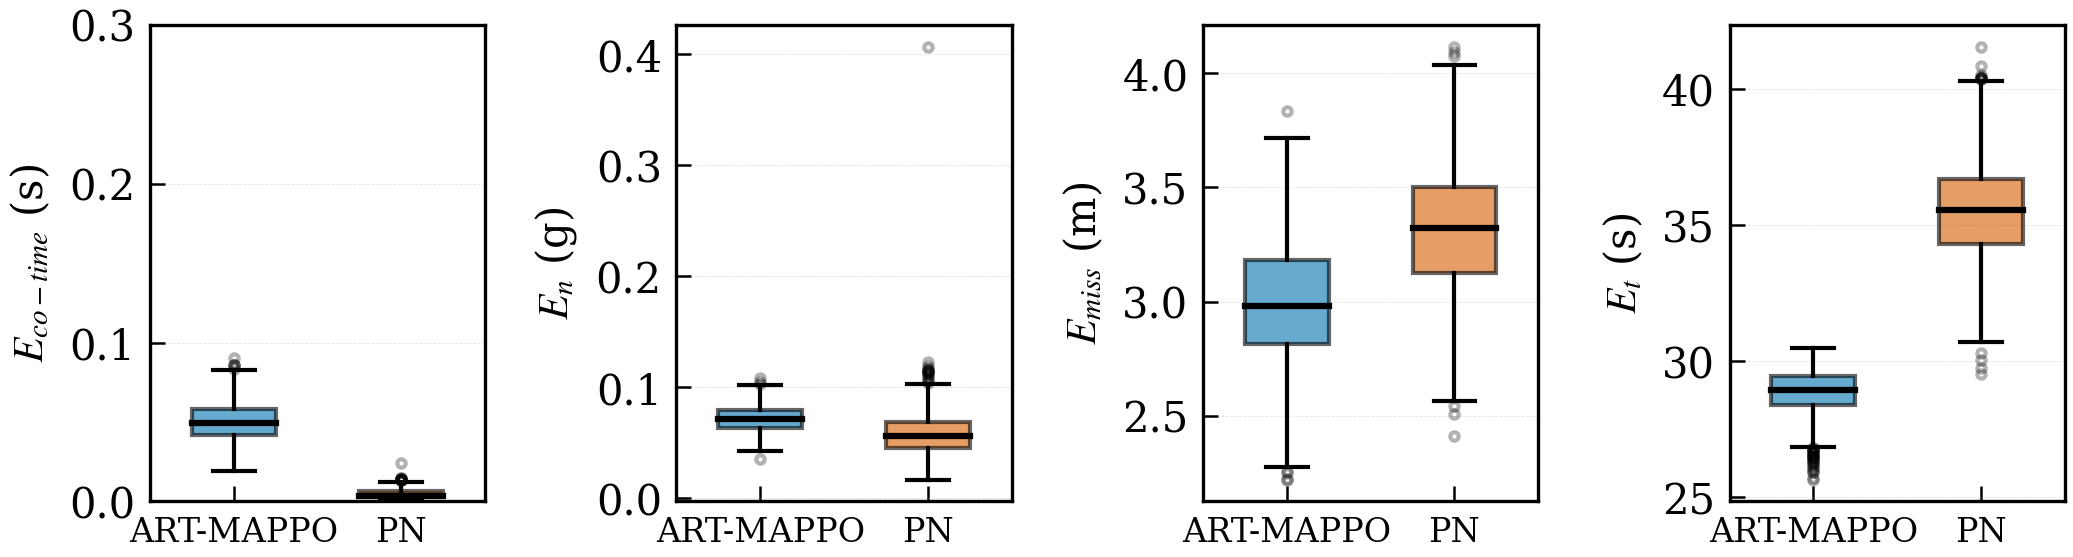
\includegraphics[width=3.5in]{nopn_mc_boxplot_compare.png}}%%%
\DIFdelendFL \DIFaddbeginFL \subfloat[Case~1]{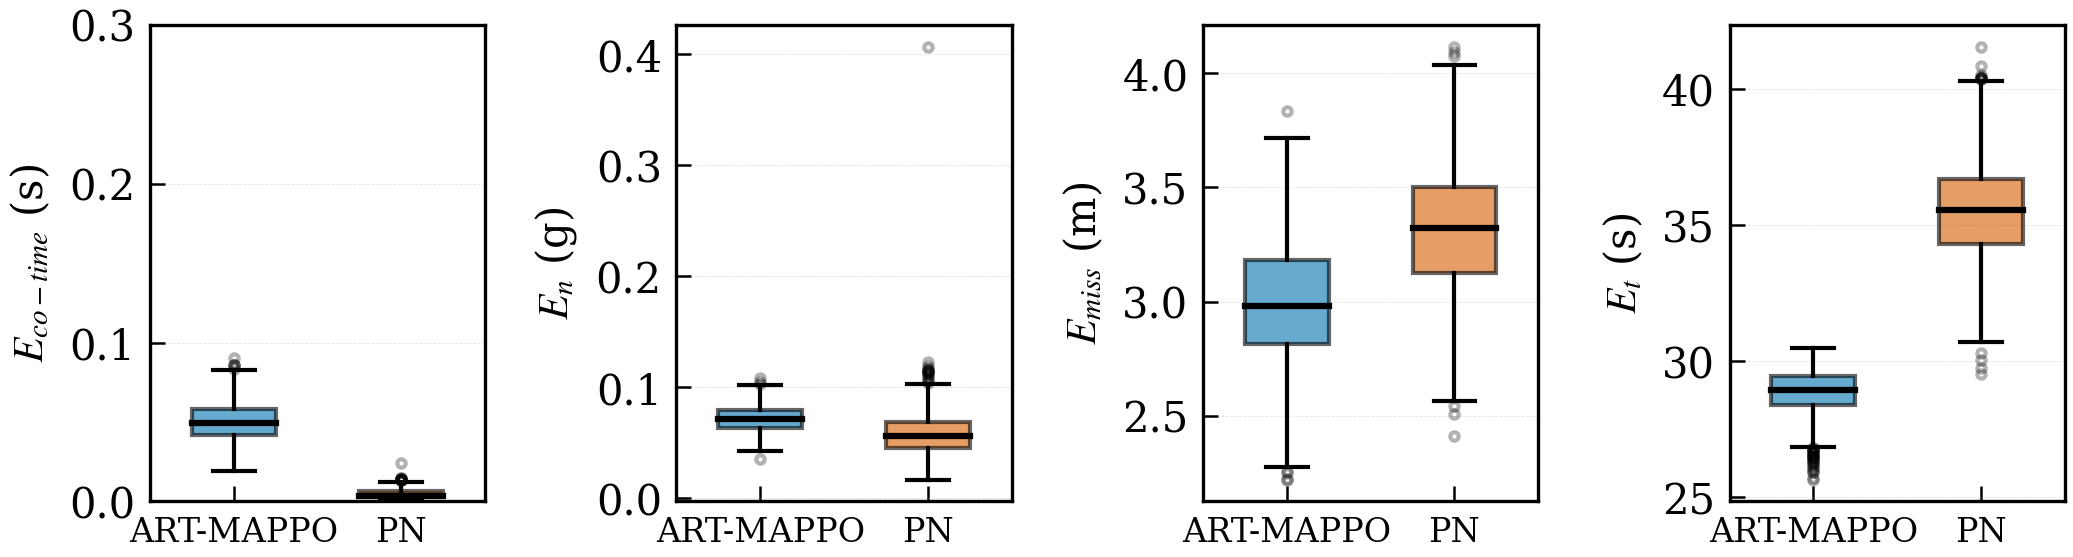
\includegraphics[width=3.42in]{nopn_mc_boxplot_compare.png}}\DIFaddendFL \\
\DIFdelbeginFL %DIFDELCMD < \subfloat[Case~2]{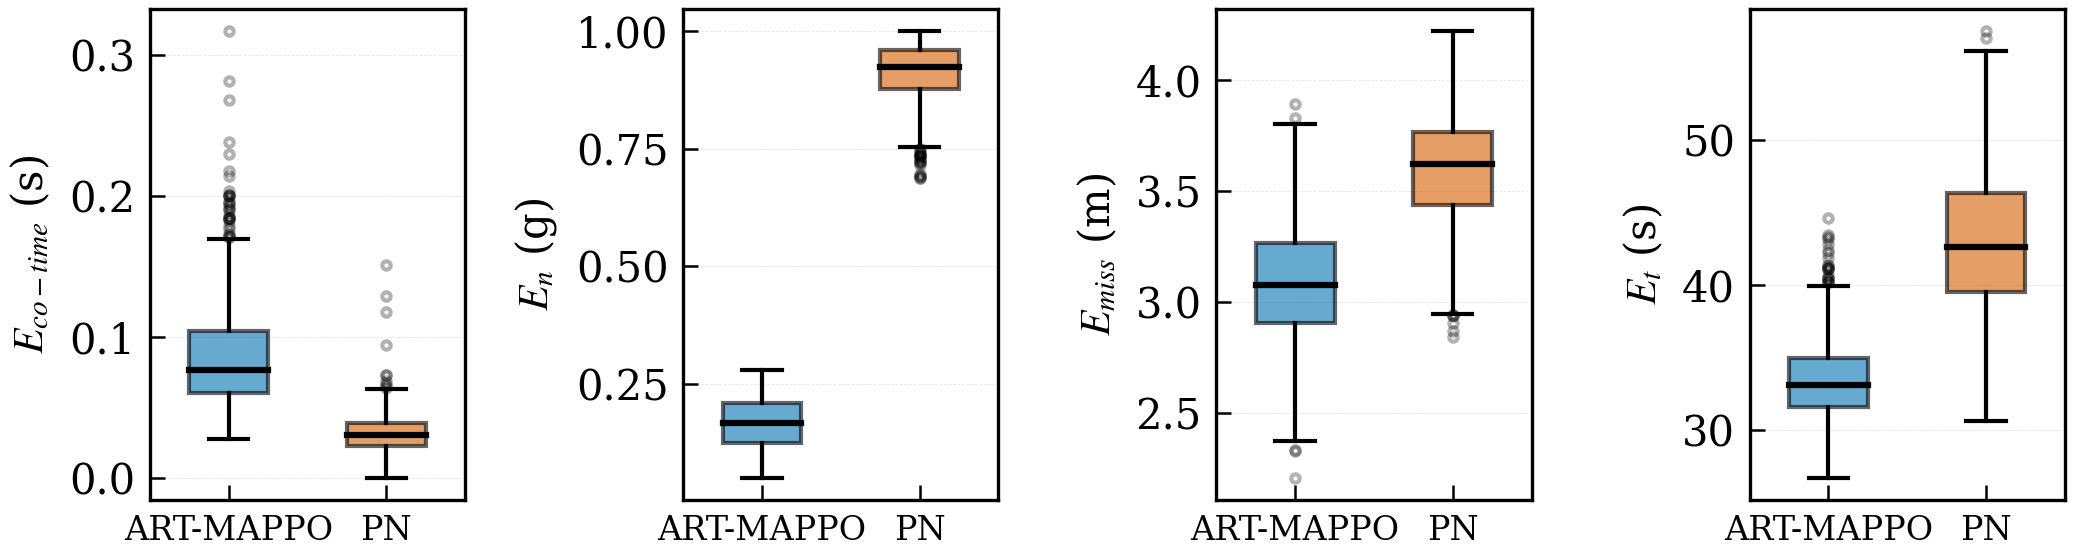
\includegraphics[width=3.5in]{sin_mc_boxplot_compare.png}}
%DIFDELCMD < %%%
\DIFdelendFL \DIFaddbeginFL \subfloat[Case~2]{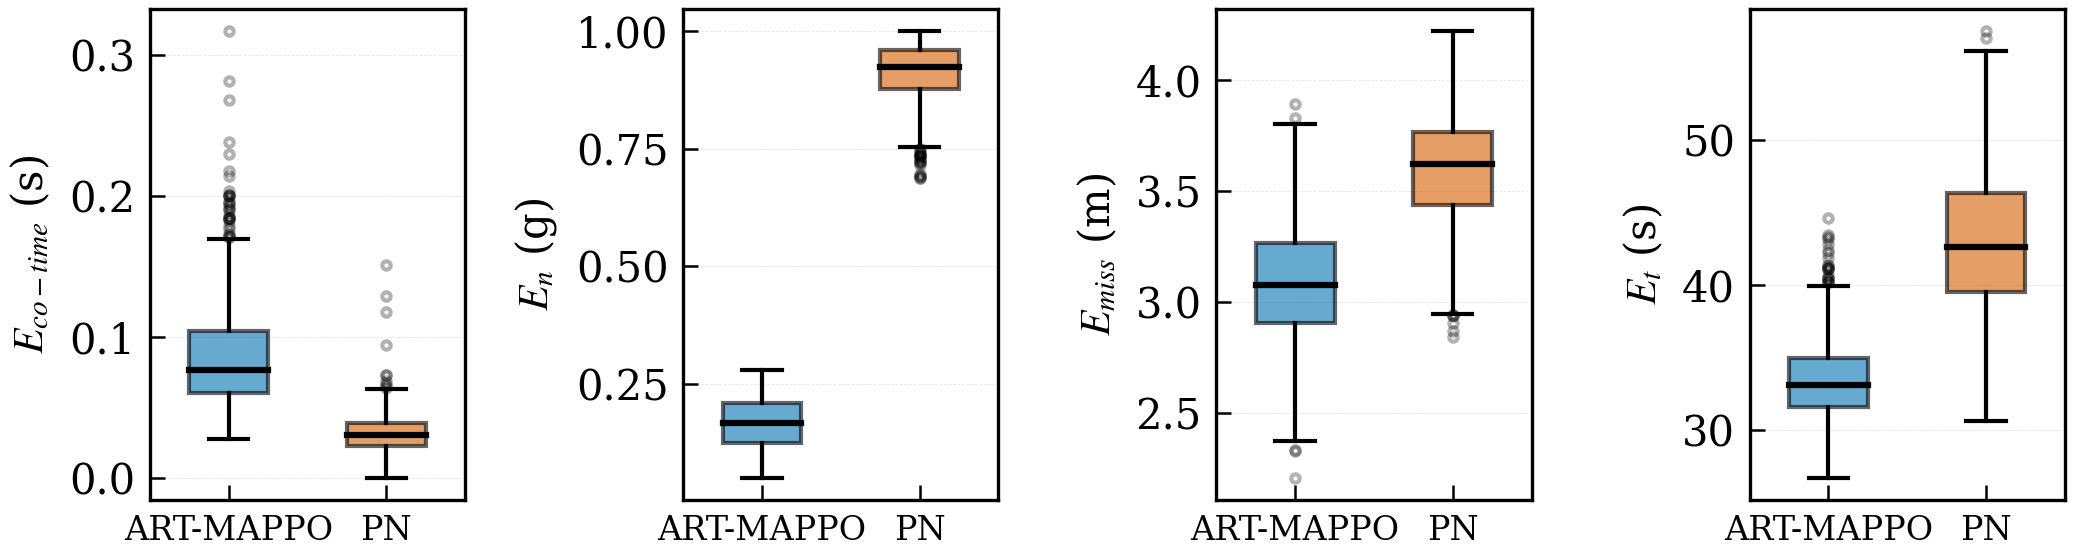
\includegraphics[width=3.42in]{sin_mc_boxplot_compare.png}}
\DIFaddendFL \caption{Boxplots of Monte Carlo trials comparing ART-MAPPO and PN (data derived from successful interceptions).}
\label{fig:mc_boxplots}
\end{figure}

Based on the statistical distributions, three key findings emerge:

\emph{(i) Interception reliability and precision.} The Interception Success Rates (ISRs) directly reflect the algorithms' adaptability to aggressive target maneuvers. While PN achieves a respectable 94.40\% against the evasive target (Case~1), its performance precipitously degrades to 17.50\% when facing the continuous weaving target (Case~2). Conversely, ART-MAPPO sustains exceptional ISRs of 98.70\% and 97.14\%, demonstrating profound robustness against continuous, high-frequency line-of-sight (LOS) oscillations. Furthermore, the $E_{miss}$ boxplots confirm that ART-MAPPO consistently achieves a lower median miss distance with a significantly narrower interquartile range (IQR), ensuring lethal precision even under worst-case initializations.

\emph{(ii) Terminal required overload and operational efficiency.} The metric $E_n$ denotes the terminal required normal overload, which is a critical constraint for flight safety. As depicted in the boxplots, ART-MAPPO's $E_n$ is tightly clustered around a safe median of $\approx0.08$\,g (Case~1) and $\approx0.20$\,g (Case~2). In stark contrast, particularly in Case~2, PN's $E_n$ distribution is heavily squeezed near the 1.0\,g upper bound. This exposes severe terminal actuator saturation, as PN struggles to reactively track the sinusoidal maneuvers. Additionally, ART-MAPPO strictly bounds the engagement duration ($E_t$) within a tight and predictable time window, reflecting superior forward energy management and rapid closure capabilities.

\emph{(iii) Robust temporal coordination.} The metric $E_{co\text{-}time}$ evaluates the temporal synchronization of the defending swarm. Across the successful Monte Carlo trials in both highly dynamic scenarios, ART-MAPPO maintains a median $E_{co\text{-}time}$ well below 0.10\,s. This consistently tight distribution confirms that the proposed algorithm can reliably shape the swarm's velocity profile to satisfy the strict temporal requirements for simultaneous saturation strikes, effectively neutralizing the risk of sequential piecemeal defeat.

\DIFaddbegin \subsection{\DIFadd{Delay, Noise, Packet Loss, and HIL Validation}}
\label{subsec:hil}

\DIFadd{The complete ART-MAPPO deployment chain was further evaluated in a
hardware-in-the-loop configuration. Policy inference and flight-control I/O
ran through hardware-connected endpoints, while target dynamics and engagement
orchestration ran in real time on the host. The HIL communication interface
applied a 100-ms observation delay, 50-ms action delay, normalized
observation/action noise standard deviations of 0.003/0.02, and 1\% command
dropout to five policy endpoints. Randomized HIL engagements used a 12-m hit
radius and a 3-s group-synchronization threshold; these criteria are stated
separately and are not mixed with the 3-m/0.5-s simulation results above.
}

\begin{table}[!t]
\centering
\caption{\DIFaddFL{HIL Temporal-State and Channel Diagnostics (10 Episodes)}}
\label{tab:hil_results}
\footnotesize
\setlength{\tabcolsep}{3pt}
\begin{tabular}{llccc}
\toprule
\DIFaddFL{Case }& \DIFaddFL{Diagnostic }& \DIFaddFL{All-hit }& \DIFaddFL{All-sync }& \DIFaddFL{Worst spread (s) }\\
\midrule
\DIFaddFL{1 }& \DIFaddFL{Full history }& \DIFaddFL{10/10 }& \DIFaddFL{10/10 }& \DIFaddFL{0.60 }\\
\DIFaddFL{1 }& \DIFaddFL{GRU reset }& \DIFaddFL{10/10 }& \DIFaddFL{10/10 }& \DIFaddFL{0.60 }\\
\DIFaddFL{1 }& \DIFaddFL{Channel impaired }& \DIFaddFL{10/10 }& \DIFaddFL{9/10 }& \DIFaddFL{43.65 }\\
\DIFaddFL{2 }& \DIFaddFL{Full history }& \DIFaddFL{10/10 }& \DIFaddFL{10/10 }& \DIFaddFL{0.20 }\\
\DIFaddFL{2 }& \DIFaddFL{GRU reset }& \DIFaddFL{10/10 }& \DIFaddFL{9/10 }& \DIFaddFL{39.55 }\\
\DIFaddFL{2 }& \DIFaddFL{Channel impaired }& \DIFaddFL{10/10 }& \DIFaddFL{10/10 }& \DIFaddFL{0.20 }\\
\bottomrule
\end{tabular}
\end{table}

\DIFadd{The GRU-reset diagnostic uses identical episode seeds but zeros the recurrent
state before every action. Its Case~2 episode~7 retains all individual hits but
synchronizes only seven of eight groups, supporting the relevance of temporal
history in that executed case. The Case~1 channel-impaired episode~6 likewise
retains 20/20 individual hits while only seven of eight groups meet the 3-s
criterion; its 43.65-s worst spread is a delayed-coordination failure and is
reported as such. A separate three-dimensional simulation with 50-ms sensing
delay, 3-m position noise, 0.3-m/s velocity noise, and a 0.30-s first-order
command lag records 20/20 hits and 8/8 synchronized groups in one selected run
for each case.
}

\DIFadd{The lightweight code example supplied with the paper co-locates compatible
endpoint interfaces in one Python process for portability. It is intended to
demonstrate policy loading and I/O, and is not the complete ART-MAPPO training,
distributed-consensus, or hardware-connected HIL experimental source.
}



\DIFaddend %% ===========================================================
\section{Conclusion}
\label{sec:conclusion}

In this paper, the cooperative interception problem of UAV swarms against highly dynamic and
maneuverable attacking UAV swarms has been investigated, explicitly accounting for real-time
decision requirements, coordinated engagement effectiveness, and terminal overload risk.
The problem is formulated by jointly considering target assignment and cooperative guidance,
and an intelligent temporally coordinated interception framework is developed.
A \DIFdelbegin \DIFdel{fast IDBO-based }\DIFdelend \DIFaddbegin \DIFadd{distributed consensus-based IDBO }\DIFaddend target assignment mechanism enables
efficient\DIFdelbegin \DIFdel{and accurate }\DIFdelend \DIFaddbegin \DIFadd{, capacity-feasible }\DIFaddend resource allocation in dynamic environments.
The ART-MAPPO cooperative guidance strategy under the CTDE paradigm improves learning
stability and training efficiency in large-scale adversarial settings.
Extensive \DIFdelbegin \DIFdel{simulations demonstrate }\DIFdelend \DIFaddbegin \DIFadd{three-dimensional simulations retain the complete two-case trajectory,
kinematic, coordination, and Monte Carlo analyses, demonstrating }\DIFaddend accelerated
target assignment, enhanced interception efficiency, improved interception
success rates, and effective alleviation of terminal overload saturation. \DIFaddbegin \DIFadd{The
hardware-connected HIL campaign further validates the deployment chain under
delay, noise, and packet loss and exposes a delayed-coordination failure that
individual-hit metrics alone would miss.
}\DIFaddend 

For future work, promising directions include cooperative interception under incomplete
information, dynamic target reassignment in unknown environments, time-constrained assignment
with explicit completion deadlines, \DIFdelbegin \DIFdel{and integration with realistic constraints such as
communication delays, limited bandwidth , and }\DIFdelend \DIFaddbegin \DIFadd{wider delay and bandwidth sweeps,
}\DIFaddend heterogeneous UAV capabilities\DIFaddbegin \DIFadd{, held-out maneuver families, and outdoor flight
validation}\DIFaddend .

% ---- Bibliography ----
\bibliographystyle{IEEEtran}
\bibliography{cja-template}

\appendices
\section{Notation Table}
\label{app:notation}

Table~\ref{tab:notation} summarizes the main symbols used in the target assignment and
ART-MAPPO formulations.

\begin{table}[!t]
\centering
\caption{Concise Notation Summary}
\label{tab:notation}
\renewcommand{\arraystretch}{1.15}
\footnotesize
\begin{tabular}{p{0.28\linewidth}p{0.62\linewidth}}
\toprule
Symbol & Description \\
\midrule
$\mathcal{U},\mathcal{T}$ & Interceptor and target sets. \\
$M,N$ & Numbers of interceptors and targets. \\
$X_{ij}$, $\mathbf{X}$ & Binary assignment variable and assignment matrix. \\
$P_{ij}$ & Interception probability weight for pair $(u_i,t_j)$. \\
$J$ & Target-assignment objective function. \\
$L_{\max}$ & Maximum number of interceptors assigned to one target. \\
$\mathbf{x}_i$ & Continuous target-preference vector of interceptor $u_i$. \\
$A_{ij}$ & Adversarial advantage for assigning $u_i$ to $t_j$. \\
$\mathcal{N}_i$ & Neighbor set of interceptor $u_i$. \\
$\mathcal{B}_i,\mathbf{c}_i,\mathbf{z}_i$ & Bundle, bid vector, and winner list in consensus bidding. \\
$\Gamma^{(k)}$ & Assignment disagreement at iteration $k$. \\
$\mathbf{o}_i^{(t)}$ & Local observation of interceptor $i$ at time step $t$. \\
$s_t$ & Centralized state used by the critic. \\
\DIFaddbeginFL \DIFaddFL{$\mathbf Q_j,\mathbf K_j,\mathbf V_j$ }& \DIFaddFL{Query, key, and value projections of attention head \(j\). }\\
\DIFaddendFL $\mathbf{h}^{(\ell)}$ & Hidden feature at the $\ell$-th network layer. \\
$\mathbf{c}_t$ & GRU hidden state for temporal encoding. \\
\DIFdelbeginFL \DIFdelFL{$a_i$ }\DIFdelendFL \DIFaddbeginFL \DIFaddFL{$a_i=[n_{x_i},n_{y_i},n_{z_i}]^\top$ }\DIFaddendFL & \DIFdelbeginFL \DIFdelFL{Continuous }\DIFdelendFL \DIFaddbeginFL \DIFaddFL{Three-dimensional }\DIFaddendFL guidance action of interceptor $i$. \\
$\pi_{\theta_i}$, $V_{\phi}$ & Decentralized actor policy and centralized value function. \\
\DIFdelbeginFL \DIFdelFL{$\mathcal{T}_i$ }\DIFdelendFL \DIFaddbeginFL \DIFaddFL{$\mathcal{T}_i,\alpha_T,\tau_T$ }\DIFaddendFL & Trust level\DIFdelbeginFL \DIFdelFL{controlling guided exploration}\DIFdelendFL \DIFaddbeginFL \DIFaddFL{, update rate, and temperature}\DIFaddendFL . \\
$r_t(\theta)$, $\hat{A}_t$ & PPO probability ratio and advantage estimate. \\
\DIFdelbeginFL \DIFdelFL{$\beta_{\mathrm{KL}}$ }\DIFdelendFL \DIFaddbeginFL \DIFaddFL{$\epsilon,c$ }\DIFaddendFL & \DIFdelbeginFL \DIFdelFL{Adaptive KL-penalty }\DIFdelendFL \DIFaddbeginFL \DIFaddFL{Standard PPO and dual-clip parameters. }\\
\DIFaddFL{$\hat D_{\mathrm{KL}},\beta_{\mathrm{KL}}$ }& \DIFaddFL{Sampled KL divergence and adaptive penalty }\DIFaddendFL coefficient. \\
$r_i^{(t)}$ & Reward of interceptor $i$ at time step $t$. \\
$\mathcal{G}_i$ & Interceptors assigned to the same target as $u_i$. \\
$E_{co\text{-}time}$, $E_n$, $E_{miss}$, $E_t$ & Coordination, terminal overload, miss-distance, and duration metrics. \\
\bottomrule
\end{tabular}
\end{table}

\end{document}
